\documentclass[a4paper,11pt]{article}
\pdfoutput=1 % if your are submitting a pdflatex (i.e., if you have
             % images in pdf, png or jpg format)

\usepackage{jcappub} % for details on the use of the package, please
                     % see the JCAP-author-manual

\usepackage[T1]{fontenc} % if needed

\title{Non-linear Structure Formation for Dark Energy Models with a Steep Equation of State}
%\title{Structure formation in a Steep Equation of State Dark Energy Cosmology }

\author[a,b,c]{N. Chandrachani Devi,}
\author[b,d]{M. Jaber-Bravo,}
\author[a]{G. Aguilar-Arg\"uello,}
\author[a]{O. Valenzuela,}
\author[a]{H. Vel\'azquez}
\author[b, e]{and A. de la Macorra}

\affiliation[a]{Instituto de Astronom\'ia, Universidad Nacional Aut\'onoma de M\'exico, A. P. 70-264, 04510, M\'exico, D.F., M\'exico\\}
\affiliation[b]{Instituto de F\'isica, Universidad Nacional Autonoma de M\'exico, Circuito de la Investigación Científica Ciudad Universitaria, 04510, M\'exico, D.F., M\'exico\\}
\affiliation[c]{Institute for Computational Cosmology, Department of Physics, Durham University, South Road, Durham, DH1 3LE, UK\\}
\affiliation[d]{
%Institute of Astronomy, UMK Piwnice k. Torunia, 87-148 Łysomice, Poland
Institute for Astronomy, Faculty of Physics, Astronomy and Informatics,  \\Nicolaus Copernicus University, Grudziadzka 5, 87-100 Toru\'n, Poland \\}
\affiliation[e]{ Instituto de Ciencias del Cosmos, University of Barcelona, ICCUB,
Barcelona 08028, Spain\\ }

% e-mail addresses: one for each author, in the same order as the authors
\emailAdd{chandrachani@gmail.com}
\emailAdd{jaber@astro.umk.pl}
\emailAdd{gaguilar@astro.unam.mx}
\emailAdd{octavio@astro.unam.mx}
\emailAdd{macorra@fisica.unam.mx}
\emailAdd{hmv@astro.unam.mx}


\abstract{
We study the non-linear regime of large scale structure formation considering a dynamical dark energy (DE) component determined by a Steep Equation of State parametrization (SEoS), $w(z)=w_0+w_i\frac{(z/z_T)^q}{1+(z/z_T)^q}$. 
In order to perform the model exploration at low computational cost, we modified the publicly available L-PICOLA code. 
We incorporate the DE model employing the first and second-order matter perturbations in the Lagrangian frame and the expansion parameter. 
We analyse deviations of dynamical DE models with respect to (w.r.t.) $\Lambda$CDM in the non-linear matter power spectrum, $P_k$, the halo mass function (HMF), and the two-point correlation function (2PCF).
We investigate the effect of a steep (SEoS-I) and smooth transition (CPL-lim) in the DE equation of state (EoS). In the former case, we found an overall impact in the $P_k$ at the level of $\sim 2-3\%$ while, for the latter, we found $\sim 3-4\%$ differences w.r.t. $\Lambda$CDM at $z=0$.
The HMF shows the possibility to distinguish between the models at the high mass end.  
For the best-fit model, dubbed  SEoS-II, we observe large deviations from $\Lambda$CDM. This is explained by the combined effect of the dynamical DE with the different amount of matter, $\Omega_{m0}$, and the higher value for $H_{0}$. 
Regarding the 2PCF, our results are relatively robust with deviations w.r.t. $\Lambda$CDM or the order $\sim 1-2 \%$ for SEoS-I and CPL-lim, and more significant deviation for SEoS-II throughout the $r$ range. Finally, we conclude that the search for viable DE models (like the SEoS) must include non-linear growth constraints.
}

\begin{document}
\maketitle
\flushbottom

\section{Introduction}
\label{sec:intro}

The unknown physics behind the observed late time accelerated expansion \cite{Roukema:1993yra, Riess:1998cb,Perlmutter:1998np} of our universe has motivated the scientific community to join their efforts in developing various spectroscopic and imaging galaxy surveys. 
These include the extended Baryon Oscillation Spectroscopic Survey (eBOSS)\footnote{https://www.sdss.org/surveys/eboss/}, the dark energy survey (DES)\footnote{https://www.darkenergysurvey.org/es/}, the Dark Energy Spectroscopic Instrument (DESI)\footnote{https://www.desi.lbl.gov/}, the Rubin Observatory Legacy Survey of Space and Time (LSST) \footnote{https://www.lsst.org/}, and the European Space Agency's Euclid \footnote{https://www.euclid-ec.org/}. They aim to measure the cosmic expansion history and the growth of structure to a precision at one percent-level. 
These huge upcoming datasets will open a window to perform several tests to discriminate between various competing cosmological models in the near future (see \cite{Santos:2016sti,Santos:2016sog,Lonappan:2017lzt} for some studies on discriminating models) and will also allow us to test gravity at the largest cosmological scales. 

So far, the concordance $\Lambda$ cold dark matter cosmological model ($\Lambda$CDM) remains as  the most successfully tested and consistent model with several observations. However, this model suffers from deep theoretical issues namely the cosmic coincidence and the fine-tunning problems, which, for instance, refers to having an exceedingly small magnitude in comparison to the expected value from fundamental physics \cite{Weinberg1989,Sahni:1999gb}. 
%
Beyond the $\Lambda CDM$ model, several alternative theories have been proposed in the literature to explain this late time cosmic acceleration \cite{Copeland:2006wr,DeFelice:2010aj,Clifton:2011jh,Joyce:2014kja}. In general, these alternative theories, either consider an exotic field with a large negative pressure called dark energy (DE) \cite{Copeland:2006wr} or modify the Einstein theory of Gravity (GR) on cosmological scales \cite{Koyama2016, Clifton:2011jh, Joyce:2014kja, Jaime:2012gc}.

Recently, various observational anomalies have arisen in the context of the $\Lambda$CDM cosmology \cite{Raveri:2015maa,Macaulay:2013swa}. 
For instance, the tension between the local value measurement of the Hubble parameter, $H_0$, and the one extrapolated from CMB measurements assuming the cosmological constant \cite{Aghanim:2018eyx}. 
It has reached up to the $5.3\sigma$ level \cite{Wong:2019kwg}. 
There is also a well known tension in the growth factor measurement, $f\sigma_{8}$, between the value measured from galaxies clustering (e.g. redshift-space distortions) and the value predicted by Planck Collaboration \cite{Macaulay:2013swa}. 
A plausible explanation may come from the correct determination of different systematic errors on those experiments. However, such tensions could also be a hint to new physics beyond the concordance $\Lambda$CDM.

There are some N-body simulations available based on dynamical DE, such as \cite{Lawrence+2017,Garrison:2017ssz, Almaraz:2019zxy}.The work of \cite{Rizzo:2016mdr} presents simulations for dynamical DE and also the case of massive neutrinos. The halo catalogs of 125 cosmological N-body simulations under the Abacus project are released in \cite{Garrison:2017ssz}, where 40 sets are based on the constant equation of state for DE ($wCDM$) model.
%of 125 cosmological DM \documentclass[a4paper,11pt]{article}
\pdfoutput=1 % if your are submitting a pdflatex (i.e., if you have
             % images in pdf, png or jpg format)

\usepackage{jcappub} % for details on the use of the package, please
                     % see the JCAP-author-manual

\usepackage[T1]{fontenc} % if needed

\title{Non-linear Structure Formation for Dark Energy Models with a Steep Equation of State}
%\title{Structure formation in a Steep Equation of State Dark Energy Cosmology }

\author[a,b,c]{N. Chandrachani Devi,}
\author[b,d]{M. Jaber-Bravo,}
\author[a]{G. Aguilar-Arg\"uello,}
\author[a]{O. Valenzuela,}
\author[b]{A. de la Macorra,}
\author[a]{and H. Vel\'azquez}


\affiliation[a]{Instituto de Astronom\'ia, Universidad Nacional Aut\'onoma de M\'exico, A. P. 70-264, 04510, M\'exico, D.F., M\'exico\\}
\affiliation[b]{Instituto de F\'isica, Universidad Nacional Autonoma de M\'exico, Circuito de la Investigación Científica Ciudad Universitaria, 04510, M\'exico, D.F., M\'exico\\}
\affiliation[c]{Institute for Computational Cosmology, Department of Physics, Durham University, South Road, Durham, DH1 3LE, UK\\}
\affiliation[d]{
%Institute of Astronomy, UMK Piwnice k. Torunia, 87-148 Łysomice, Poland
Institute for Astronomy, Faculty of Physics, Astronomy and Informatics,  \\Nicolaus Copernicus University, Grudziadzka 5, 87-100 Toru\'n, Poland
}

% e-mail addresses: one for each author, in the same order as the authors
\emailAdd{chandrachani@gmail.com}
\emailAdd{jaber@astro.umk.pl}
\emailAdd{gaguilar@astro.unam.mx}
\emailAdd{octavio@astro.unam.mx}
\emailAdd{macorra@fisica.unam.mx}
\emailAdd{hmv@astro.unam.mx}


\abstract{
We study the non-linear regime of large scale structure formation considering a dynamical dark energy (DE) component determined by a Steep Equation of State parametrization (SEoS), $w(z)=w_0+w_i\frac{(z/z_T)^q}{1+(z/z_T)^q}$. 
In order to perform the model exploration at low computational cost, we modified the publicly available L-PICOLA code. 
We incorporate the DE model employing the first and second-order matter perturbations in the Lagrangian frame and the expansion parameter. 
We analyse deviations of dynamical DE models with respect to (w.r.t.) $\Lambda$CDM in the non-linear matter power spectrum, $P_k$, the halo mass function (HMF), and the two-point correlation function (2PCF).
We investigate the effect of a steep (SEoS-I) and smooth transition (CPL-lim) in the DE equation of state (EoS). In the former case, we found an overall impact in the $P_k$ at the level of $\sim 2-3\%$ while, for the latter, we found $\sim 3-4\%$ differences w.r.t. $\Lambda$CDM at $z=0$.
The HMF shows the possibility to distinguish between the models at the high mass end.  
For the best-fit model, dubbed  SEoS-II, we observe large deviations from $\Lambda$CDM. This is explained by the combined effect of the dynamical DE with the different amount of matter, $\Omega_{m0}$, and the higher value for $H_{0}$. 
Regarding the 2PCF, our results are relatively robust with deviations w.r.t. $\Lambda$CDM or the order $\sim 1-2 \%$ for SEoS-I and CPL-lim, and more significant deviation for SEoS-II throughout the $r$ range. Finally, we conclude that the search for viable DE models (like the SEoS) must include non-linear growth constraints.
}

\begin{document}
\maketitle
\flushbottom

\section{Introduction}
\label{sec:intro}

The unknown physics behind the observed late time accelerated expansion \cite{Roukema:1993yra, Riess:1998cb,Perlmutter:1998np} of our universe has motivated the scientific community to join their efforts in developing various spectroscopic and imaging galaxy surveys. 
These include the extended Baryon Oscillation Spectroscopic Survey (eBOSS)\footnote{https://www.sdss.org/surveys/eboss/}, the dark energy survey (DES)\footnote{https://www.darkenergysurvey.org/es/}, the Dark Energy Spectroscopic Instrument (DESI)\footnote{https://www.desi.lbl.gov/}, the Rubin Observatory Legacy Survey of Space and Time (LSST) \footnote{https://www.lsst.org/}, and the European Space Agency's Euclid \footnote{https://www.euclid-ec.org/}. They aim to measure the cosmic expansion history and the growth of structure to a precision at one percent-level. 
These huge upcoming datasets will open a window to perform several tests to discriminate between various competing cosmological models in the near future (see \cite{Santos:2016sti,Santos:2016sog,Lonappan:2017lzt} for some studies on discriminating models) and will also allow us to test gravity at the largest cosmological scales. 

So far, the concordance $\Lambda$ cold dark matter cosmological model ($\Lambda$CDM) remains as  the most successfully tested and consistent model with several observations. However, this model suffers from deep theoretical issues namely the cosmic coincidence and the fine-tunning problems, which, for instance, refers to having an exceedingly small magnitude in comparison to the expected value from fundamental physics \cite{Weinberg1989,Sahni:1999gb}. 
%
Beyond the $\Lambda CDM$ model, several alternative theories have been proposed in the literature to explain this late time cosmic acceleration \cite{Copeland:2006wr,DeFelice:2010aj,Clifton:2011jh,Joyce:2014kja}. In general, these alternative theories, either consider an exotic field component with a large negative pressure called dark energy (DE) \cite{Copeland:2006wr} or modify the Einstein theory of Gravity (GR) on cosmological scales \cite{Koyama2016, Clifton:2011jh, Joyce:2014kja, Jaime:2012gc}.

Recently, various observational anomalies have arisen in the context of the $\Lambda$CDM cosmology \cite{Raveri:2015maa,Macaulay:2013swa}. 
For instance, the tension between the local value measurement of the Hubble parameter, $H_0$, and the one extrapolated from CMB measurements assuming the cosmological constant \cite{Aghanim:2018eyx}. 
It has reached up to the $5.3\sigma$ level \cite{Wong:2019kwg}. 
There is also a well known tension in the growth factor measurement, $f\sigma_{8}$, between the value measured from galaxies clustering (e.g. redshift-space distortions) and the value predicted by Planck Collaboration \cite{Macaulay:2013swa}. 
A plausible explanation may come from the correct determination of different systematic errors on those experiments. However, such tensions could also be a hint to new physics beyond the concordance $\Lambda$CDM.

There are some N-body simulations available based on dynamical DE, such as \cite{Lawrence+2017,Garrison:2017ssz, Almaraz:2019zxy}.The work of \cite{Rizzo:2016mdr} presents simulations for dynamical DE and also the case of massive neutrinos. The halo catalogs of 125 cosmological N-body simulations under the Abacus project are released in \cite{Garrison:2017ssz}, where 40 sets are based on the constant equation of state for DE ($wCDM$) model.
%of 125 cosmological DM N-body simulations under the Abacus project where 40 sets are based on the constant equation of state DE ($wCDM$) model. % are released in \cite{Garrison:2017ssz} where 40 sets are based on the constant equation of state DE ($wCDM$) model with Planck 2015 cosmology.
 %in 1.1 $h^{-1}$ Gpc and $720 h^{-1}$ Mpc boxes. 
 %The halo catalogues and particles subsamples ranging from z = 1.5 to 0.1 are publicly available \footnote{https://lgarrison.github.io/AbacusCosmos.}.
\cite{Lawrence+2017} provided the results of the Chevallier-Polarski-Linder (CPL) parameterization \cite{Chevallier2001,Linder2003} for DE, including also massive neutrinos. The latter was run with the Hardware-Hybrid Cosmology Code (HACC), a high-performance cosmology code (see \cite{Heitmann:2015xma} for more details).

In addition to the high-resolution N-body simulations, several fast-approximated N-body simulations have been developed to mock the galaxy catalogs accurately on vast scales. % and at fast rate.
However, their primary goal is to estimate the covariance matrix accurately for large scale structure surveys, and so they use the standard $\Lambda$CDM model. 
%
The list includes PTHalos \cite{Scoccimarro:2001cj}, Quick Particle Mesh Simulations(QPM) \cite{White:2013psd}, Effective Zel'dovich approximation mocks(EZmocks) \cite{Chuang:2014vfa}, PINOCCHIO \cite{Monaco:2001jg, Monaco:2013qta}, PATCHY \cite{2014MNRAS.439L..21K}, COmoving Lagrangian Acceleration (COLA) \cite{Tassev:2013pn,Tassev:2015mia}, an upgraded light cone enabling parallel version of COLA: L-PICOLA \cite{Howlett:2015hfa}, etc.  Each of them has its own approximation methods and applications on mocking the catalogs and analyzing uncertainties on several on-going surveys. 

 
For our purpose, we employ the L-PICOLA code\cite{Howlett:2015hfa} after incorporating the dynamical DE through the expansion history, first and second-order Lagrangian Perturbation Theory (2LPT) approximation. The COLA method used in \cite{Howlett:2015hfa} was introduced with an idea to capture the large scale structure (LSS) accurately within few time steps, with the less use of computational resources but still enabled to small scales  accurately  \cite{Tassev:2013pn,Tassev:2015mia}. It is done successfully by implementing the solutions of the first and second-order dark matter perturbations that guarantee to capture the LSS to some extent. Along with this idea of COLA and the large number of cosmological models we have, the implementation of such models in fast COLA-like N-body simulations would be an efficient and adequate way to understand their effects in the regimes required for the upcoming galaxy surveys.
 
An attempt in this regard has already made for the modified gravity(MG) theories in the referred code called MG-COLA \cite{Winther:2017jof}.
Their studies pointed out that, in general, the COLA approach overestimates the halo mass function even for the $\Lambda$CDM model but preserving the difference of MG w.r.t. $\Lambda$CDM accurately. For our case, we are choosing the dynamical DE models of CPL-like parameterization  \cite{Chevallier2001,Linder2003} and the steep equation of state parameterization \cite{Jaber:2017bpx}. We perform a comparative study w.r.t. $\Lambda$CDM. The main idea of this work is not only to understand the effect of these DE models but also to confront our understanding in disentangling their effect from the global cosmological parameters such as $\Omega_{m0}$ and $H_{0}$, through LSS.

The paper is structured as follows: In Section \ref{sec:method}, we describe the models, their background evolution, and the dark matter perturbations up to second-order (see \cite{Bernardeau:2001qr} for a review). In Section \ref{sec:nonlinear}, we discuss the COLA method employed by the N-body simulation called L-PICOLA \cite{Howlett:2015hfa}. The results in terms of the dark matter power spectrum, the halo mass function, and the two-point correlation function of halos are discussed in section  \ref{sec:results}. We summarise and conclude in Section \ref{sec:conclusions}.

The fiduciary cosmological parameters used for this work are $\Omega_{m0} = 0.3089$, $\Omega_{b0} = 0.045$, $h = 0.6774$, $\sigma_{8} = 0.8159$,and $n_s = 0.9667$.

\section{Cosmological models}
\label{sec:method}
This section focuses on the DE models we considered for our analysis. We discuss their background expansion history and the evolution of their matter perturbations up to second-order. Such perturbative solutions are used in generating the initial conditions for the N-body simulations. 

\subsection{Dark energy model and background expansion}
\label{sec:background}

\begin{figure}
\centering 
%\hfill
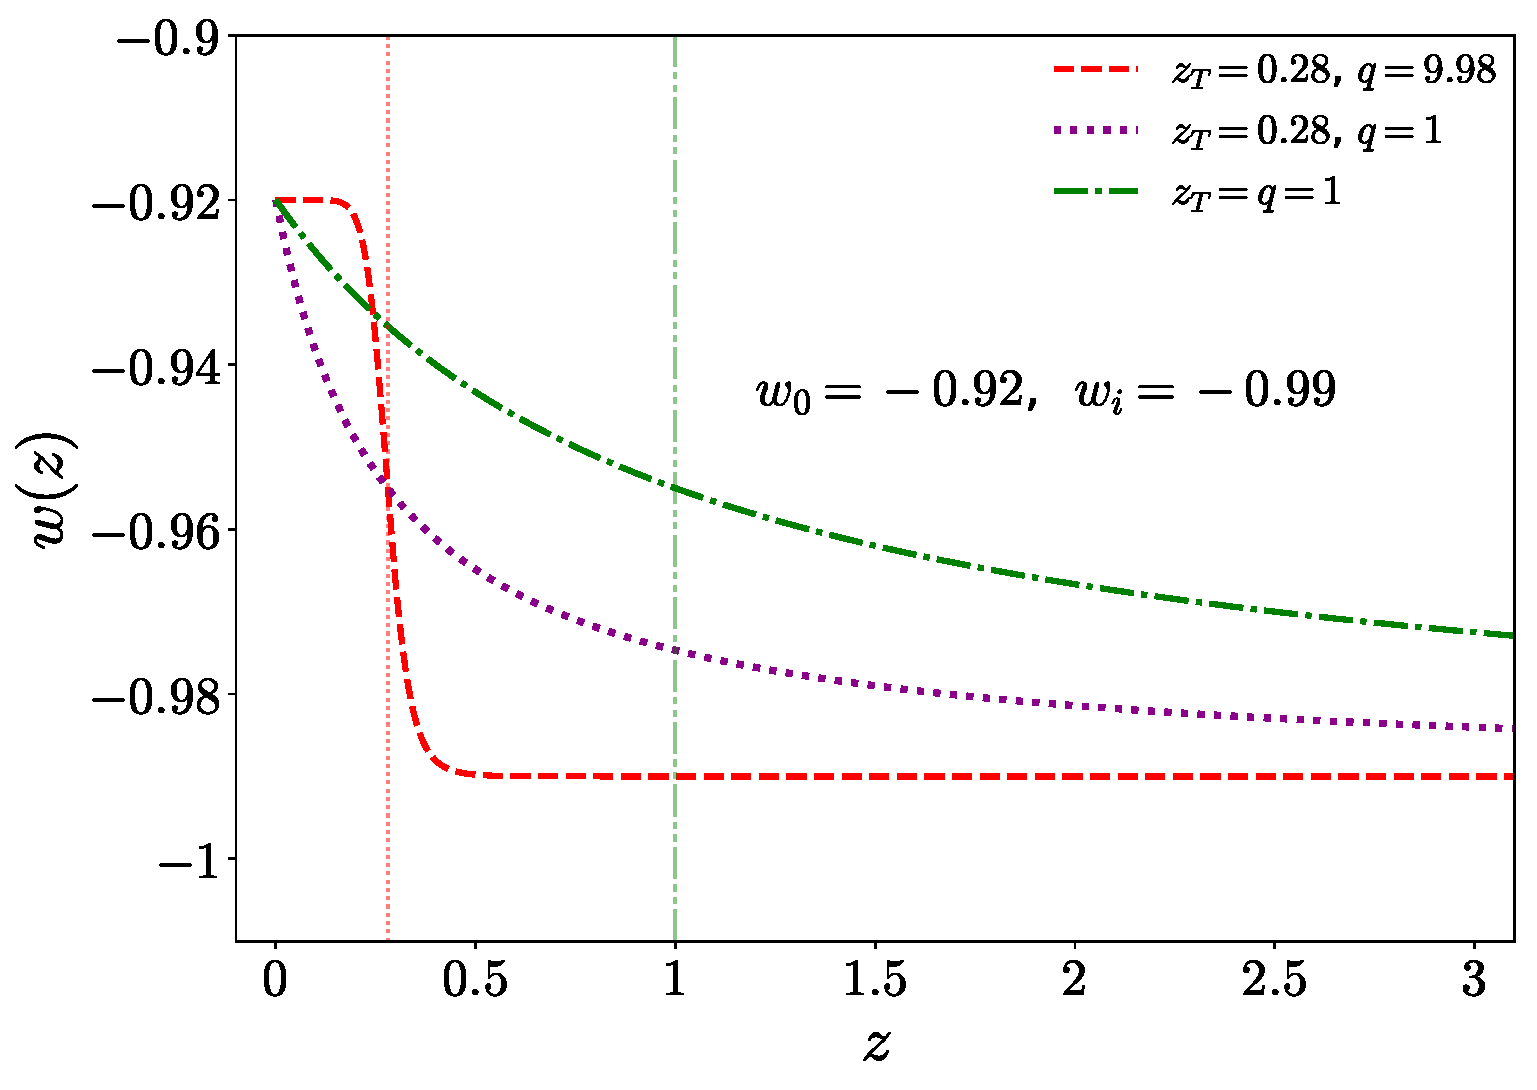
\includegraphics[width=0.6\textwidth, angle=0]{./plots/fig1_2a.pdf}
\caption{\label{fig:eosqs} Evolution of the proposed equation of state for DE  \eqref{eq:seos} with fixed parameters $w_0=-0.92$, $w_i=-0.99$. The red dashed line corresponds to $z_T=0.28$ and $q=9.98$ which we refer to as SEoS-I hereafter. The green dot-dashed line with $q=z_T=1$ represents the CPL limit of SEoS model with the CPL parameters: $w_0 =-0.92$ and $w_a =-0.07$. The magenta dotted line with $z_T=0.28$ and $q=1$ represents an intermediate case between them. The transition between two pivotal points is marked with the vertical lines for SEoS-I and CPL limit that are occurring at $z_T=0.28$  and $z_T=1$, respectively. The value $z_T$ is defined as $z$ where $w(z_T) = (w_0+w_i)/2$.% Focusing at redshift $z=0.28$, the difference of $\sim 4\%$ is observed between SEoS-I and $\Lambda$CDM whereas CPL has $\sim 7\%$. Similarly at $z=1$, the difference for SEoS and CPL limit reduces to $\sim 1\%$ and $\sim 5\%$ respectively. After $z=0.5$, the SEoS remains to be within $1\%$ throughout redshifts while CPL limit becomes $3\%$ only after $z=2$. For redshifts $z\geq10$, all models displayed are of the order $1\%$ difference from $\Lambda$CDM.
}
\end{figure}

In a phenomenological approach, dark energy models are parametrized through its equation of state (EoS), $w(z) \equiv \frac{{\rm p_{DE}}(z)}{{\rm \rho_{DE}}(z)}$, which describes the evolution of DE pressure to its density as a function of time within a set of free parameters. 
Several forms of $w(z)$ have been proposed in the literature, (see for instance, \cite{Chevallier:2000qy, Linder2003, Doran:2006kp, KraussJonesHuterer2007, Linder:2006ud, Rubin:2008wq, 2009ApJ:703:1374S, 2010PhRvD..81f3007M, Hannestad:2004cb, Jassal:2004ej, Ma:2011nc, Huterer:2000mj, Weller:2001gf, Huang:2010zra, Barboza:2008rh}). 
 Among them, the so-called Chevallier-Polarski-Linder (CPL) parameterization \cite{Chevallier2001,Linder2003} is one of the most widely studied parameterization to the DE equation of state and is given by:
\begin{equation}
w(z) =w_{0}+w_{a}\frac{z}{1+z},
\label{eq:wcpl}
\end{equation}
where $w_{0}$ and $w_{a}$ are constant parameters representing the present value of the EoS and its overall time evolution, respectively. Current observational constrains on CPL parameters are presented in \cite{Linden:2008mf}. 

Within the framework of General Relativity, for a late-time, flat, homogeneous and isotropic universe (i.e.,  governed by the FLRW metric), filled with non-relativistic dark matter (DM) and the DE component, i.e.,  $\Omega_{DE} + \Omega_{m} = 1$, the Hubble expansion rate is governed by
\begin{equation}
\frac{H(z)^2}{H_{0}^2} = \Omega_{m0} (1+z)^{3} + (1- \Omega_{m0}) F(z),
\label{eq:hubble}
\end{equation}
where $H_{0}$ and $\Omega_{m0}$ represent the present day values of Hubble rate and matter density, respectively. The DE density, $\Omega_{DE}(z) = (1-\Omega_{m0})F(z)$ evolves with redshift, $z$ as 
\begin{equation}
F(z) = \exp\left[3 \int_{0}^{z} (1+w(z^{\prime}))/(1+z^{\prime})dz^{\prime}\right].
\label{eq:CPL}
\end{equation}
%\textcolor{gray}{}
In this work, we consider a more general EoS of DE other than \eqref{eq:wcpl}, inspired by  quintessence fields dynamics \cite{delaMacorra:2015aqf}, a parametrization described by:
%
\begin{equation}
\label{eq:seos}
w(z) = w_0 + (w_i-w_0)\frac{\left(z/z_T \right)^q}{1+\left(z/z_T \right)^q}.
\end{equation}
%
where $w_i$ and $w_0$ represent the value of $w(z)$ at high redshifts and at present day, respectively. Here the function, $f(z) = \frac{\left(z/z_T \right)^q}{1+\left(z/z_T \right)^q}$ with a transition redshift, $z_{T}$, and a steepness parameter, $q$, governs the dynamics of the parametrization between two pivotal values ($w_i$,$w_0$). For instance, in case of $f(z) =0$ at $z=0$, EoS becomes $w(z) = w_{0}$; at $ z -> \infty$ where $f(z) =1$, $w(z) = w_{i}$ and at $z =z_T$ where $f(z) = 1/2$, then $w(z) = (w_0+ w_i)/2$. This gives us the range of $f(z)$ values, i.e., $0 < f(z) < 1$. 

Note that $q$ determines the steepness of transition. With a large value of $q$, an abrupt transition with a shorter period of transition is expected and vice-versa. For this reason we dubbed the parameterization as a “Steep Equation of State,” hereafter referred to as SEoS. Interestingly, we recover the well-known CPL model  \eqref{eq:CPL} with a smooth transition at $z_T = 1$ for $q=1$, where the CPL parameters relate with SEoS parameters via $w_a\equiv w_i-w_0$.
We further consider this particular case with ($w_0 = -0.92$, $w_i = -0.99$) and $z_T=q= 1$ as our “CPL limit” for comparison of different DE models.
The proposed parameterization of the EoS also recovers the standard $\Lambda$CDM model in the limit of $w_0 = w_i = -1$ for any values of $q$ and $z_T$.

Figure (\ref{fig:eosqs}) shows the evolution of $w(z)$ for the proposed SEoS parameterization with its free parameters fixed to the best fit values found in \cite{Jaber:2017bpx}: $\{w_0, w_i, q, z_T\} = \{-0.92,-0.99,9.98,$ $0.28\}$ (red dashed line), refer as SEoS-I along with slightly varying values of $(q, z_{T})$. The corresponding CPL limit (CPL-lim) with its parameters: $w_0 =-0.92$ and $w_a =-0.07$ is presented with the green dot-dashed line. For the same values of ($w_0, w_i, z_T$) but with $q=1$, we have different behavior, shown in the magenta dotted line, which is an intermediate case between the preceding two cases.  The transition redshift, $z_T$ between two pivotal points $(w_0, w_i)$ for SEoS-I and CPL-lim are marked by the vertical lines that occur at $z_T=0.28$  and $z_T=1$, respectively. 


One can see from the Figure (\ref{fig:eosqs}) that $w(z)$ with $q=9.98$ (red dashed line) transits from a $0.1\%$ difference w.r.t. $\Lambda$CDM to roughly $8\%$ in the interval of $\Delta z \sim 0.2$, presenting a rapid dilution of the DE density. 
%and the difference in $w(z)$ from $\Lambda$CDM transits from $\sim 0.1\%$ to $\sim 8\%$.  
While in CPL-lim (green dash line) with $q = 1$, the transition occurs from $\sim 0.3\%$ to $\sim 8\%$ difference in the interval of $\Delta z \sim 2$, clearly depicting how smooth the transition can be depending on the values of $q$. For more details for the EoS behaviors, we refer to Figure(1) of \cite{Jaber:2019opg}.
 

In Table (\ref{table:COLA_models}) we summarize the considered models. The SEoS-I and CPL-lim  cases refer to SEoS model with  $\{w_0, w_i, q, z_T\} = \{-0.92, -0.99, 9.98, 0.28\}$ and its CPL limit, respectively, both with the global cosmological parameters based upon the Planck collaboration (P15)\cite{Ade2016} as for $\Lambda$CDM. The SEoS-II model is defined with the same set of parameters $\{w_0, w_i, q, z_T\} = \{-0.92,-0.99, 9.98,0.28\}$ but with the best fit values of $H_{0}$ and $\Omega_{m0}$ from \cite{Jaber:2017bpx}, i.e.,  $H_{0}=73.22$ and $\Omega_{m0} =0.334$. 
In \cite{Jaber:2017bpx}, the SEoS-II case was found to be the best model fitting observations of the Baryonic acoustic peak from galaxies (\cite{Beutler:2011hx,Ross:2014qpa,Padmanabhan2pc,Alam:2016hwk}) and Lymann-$\alpha$ forest (\cite{Font-Ribera:2013wce,Delubac:2014aqe}) along with the local determination of the Hubble parameter $H_0$ from \cite{Riess:2016jrr}.

Their analysis found $1\sigma$ constraints on the parameters: $w_0=-0.92^{+0.15}_{-0.14}$, $w_i=-0.99(\leq-0.67)$. The parameters $q$ and $z_T$ had weaker $1\sigma$ constraints using those data sets: $q=9.98 (\geq 7.19)$ and $z_T=0.28(\leq 1.08)$.

The corresponding Hubble expansion rates for the models presented in table (\ref{table:COLA_models}) are shown in Figure (\ref{fig:hubble_ratios}). The solid black, red dashed, green dot-dashed, and blue dotted lines represent the $\Lambda$CDM, SEoS-I, CPL-lim, and SEoS-II cases, respectively. We keep this convention throughout the paper. 

From the lower panel of Figure (\ref{fig:hubble_ratios}) we can see that all models have a similar expansion rate. In particular, SEoS-I and CPL-lim cases 
converge to the same $H(z)$ value at $z=0$ since they share the same  cosmological parameters as in $\Lambda$CDM. However, in CPL-lim, the transition occurs at higher redshift in comparison to SEoS-I, so it starts to deviate from $\Lambda$CDM slightly earlier then SEoS-I. However, the expansion rate, $E(a) =H(a)/H_{0}$, of SEoS-I and CPL-lim remains within $\sim 1\%$ difference from $\Lambda$CDM  and deviates by $\sim 2\%$ around the epoch of the transition ($z_{T} = 0.28, 1$, respectively). In case of SEoS-II, more relevant than the  SEoS parameters, the difference in the values of $H_0$ and $\Omega_{m0}$, induces discrepancies from $\Lambda CDM$ throughout all the redshift values. In particular, we notice that at present day, the value for $H(z)$ is $\sim 8\%$ larger than in $\Lambda CDM$ and the difference goes up to $12\%$ at higher redshifts. 


\begin{figure}
\centering 
%\hfill
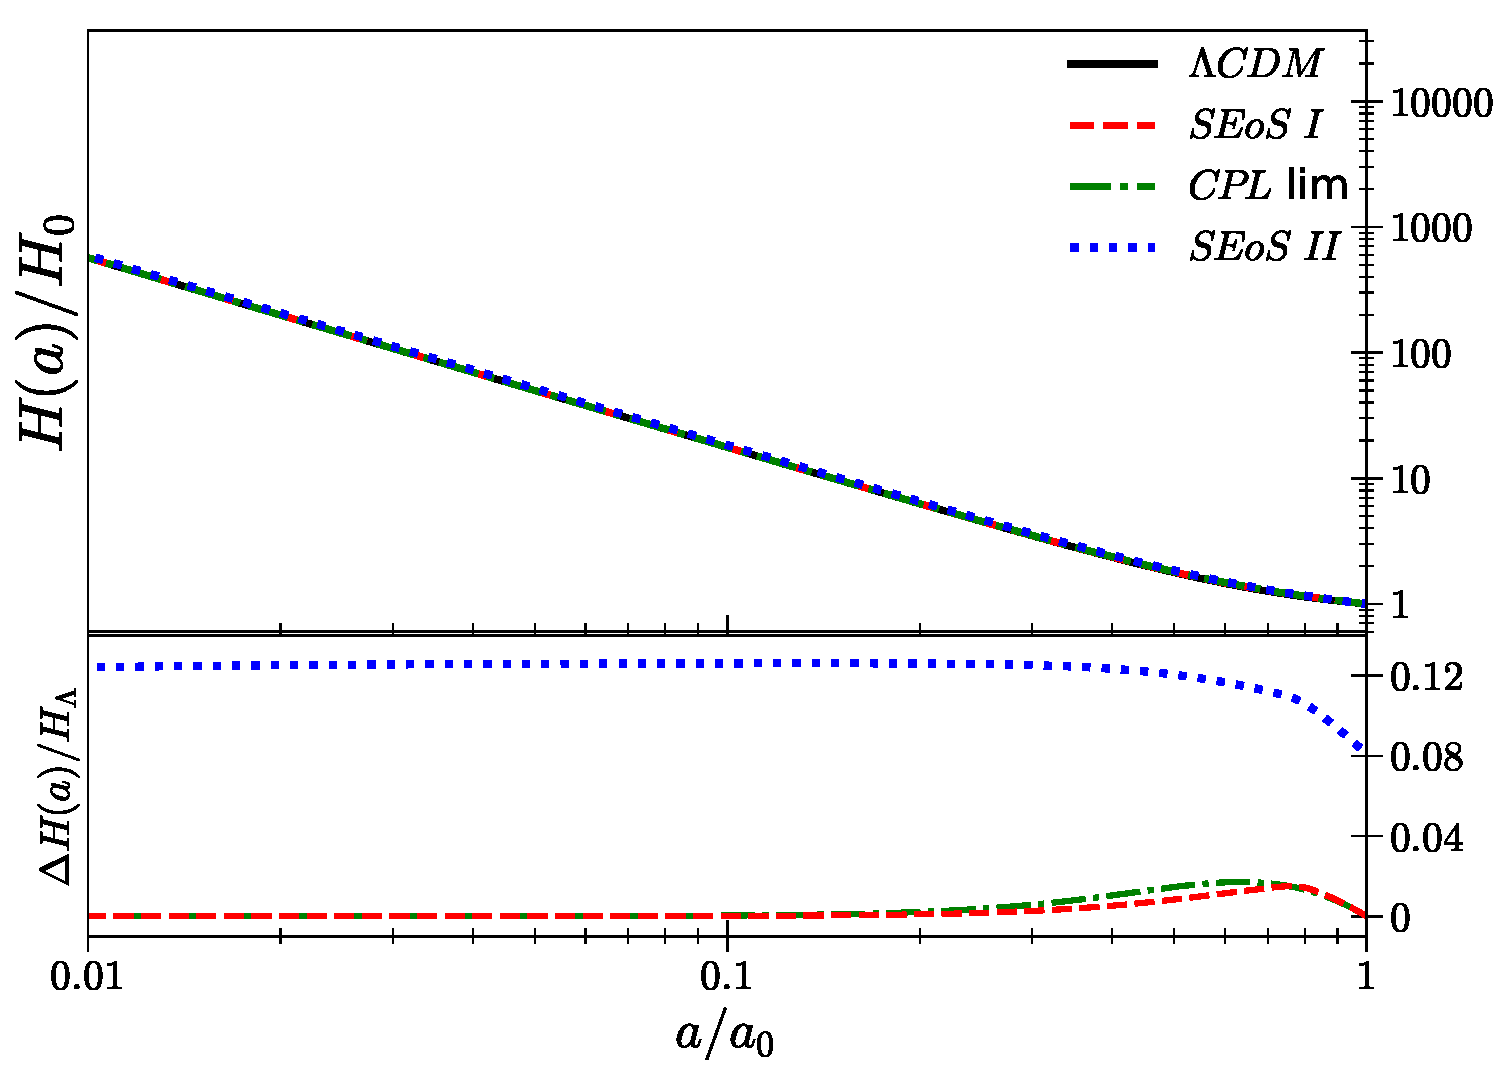
\includegraphics[width=0.6\textwidth,angle=0]{./plots/H_of_a_4_models_ratio.pdf}
\caption{\label{fig:hubble_ratios}{\it Upper panel}: Normalized Hubble expansion rate for the models we consider (listed in Table \ref{table:COLA_models}).  
{\it Bottom panel}: The relative difference w.r.t. $\Lambda$CDM: $\Delta H/H_{\Lambda} \equiv (H/H_{\Lambda} -1)$. Since cases SEoS-I (red dash line), $CPL$-lim (green dotted-dash line), and $\Lambda$CDM (black solid line) share the same values of $H_0$ and $\Omega_{m0}$, they converge to the same $H(z=0)$. CPL-lim has a transition redshift at $z_T=1$, which is larger compared to the one for SEoS case, $z_T=0.28$, and therefore, it shows a departure from $\Lambda CDM$ at a smaller $a/a_0$ value. Since in the SEoS-II case, we have different $H_0$ and also the amount of matter, a discrepancy w.r.t. $\Lambda CDM$ is observed throughout all time scales. This convention in labels for the different models is used throughout the Figures.} 
\label{figure:hubble}
\end{figure}

\begin{figure*}
     \centering
     \begin{tabular}{cc}
        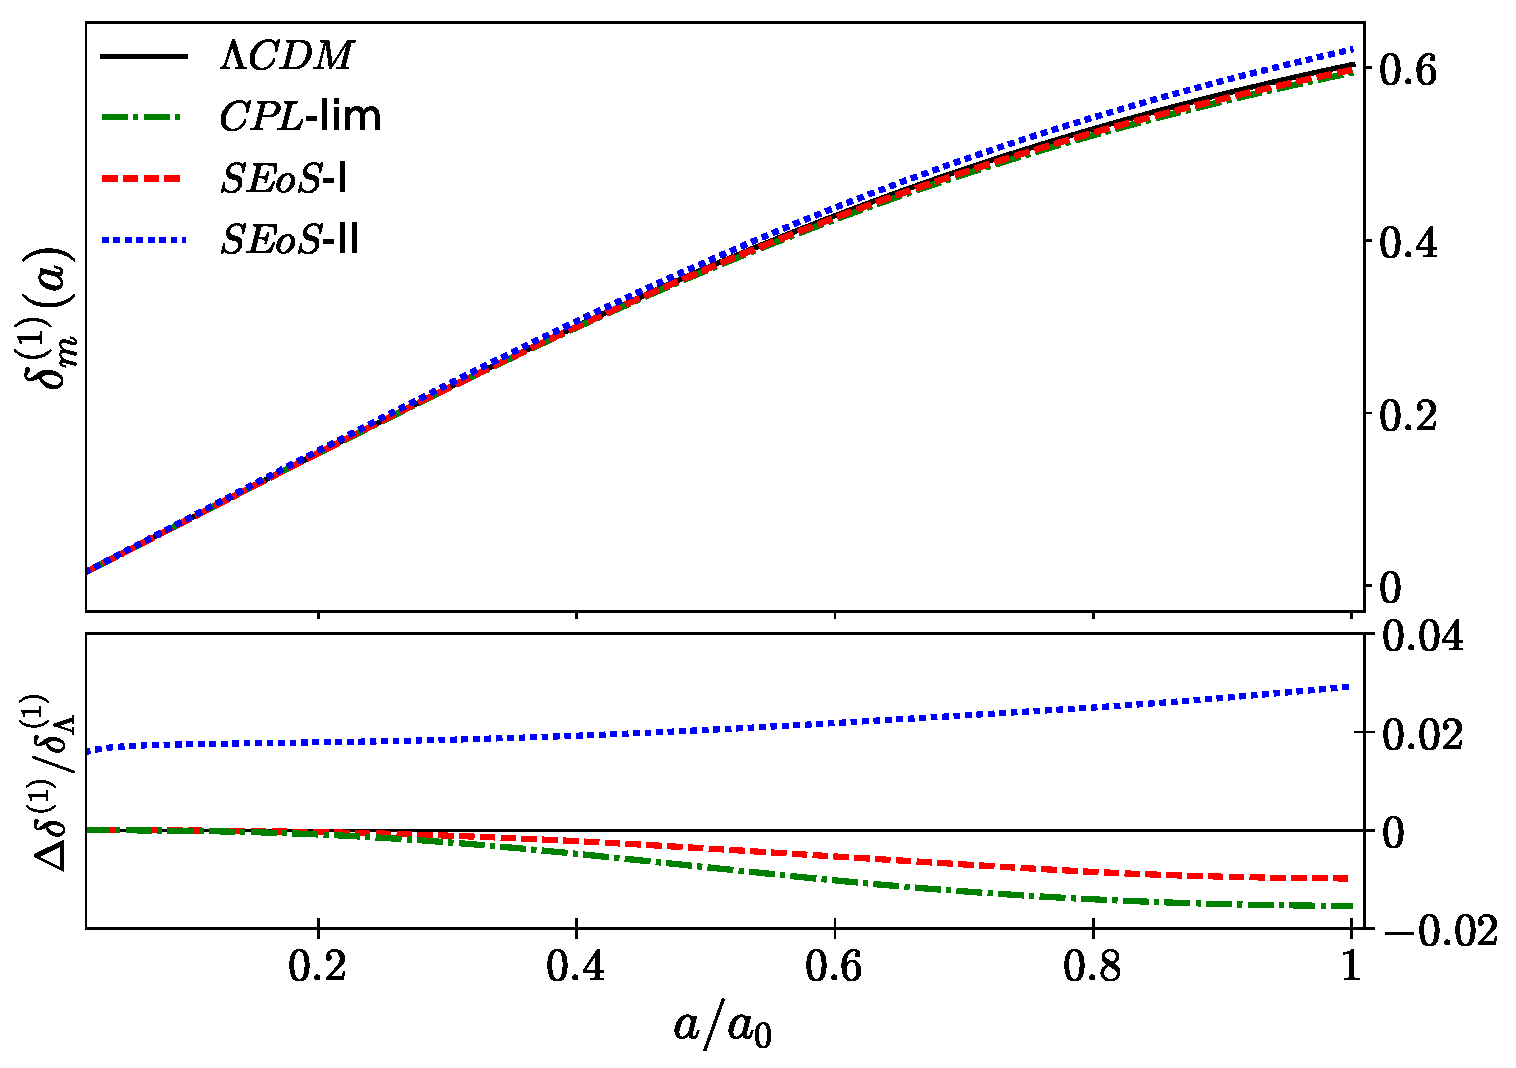
\includegraphics[width=0.49\textwidth,angle=0]{./plots/d1m_4models_ratio_linlin}   
        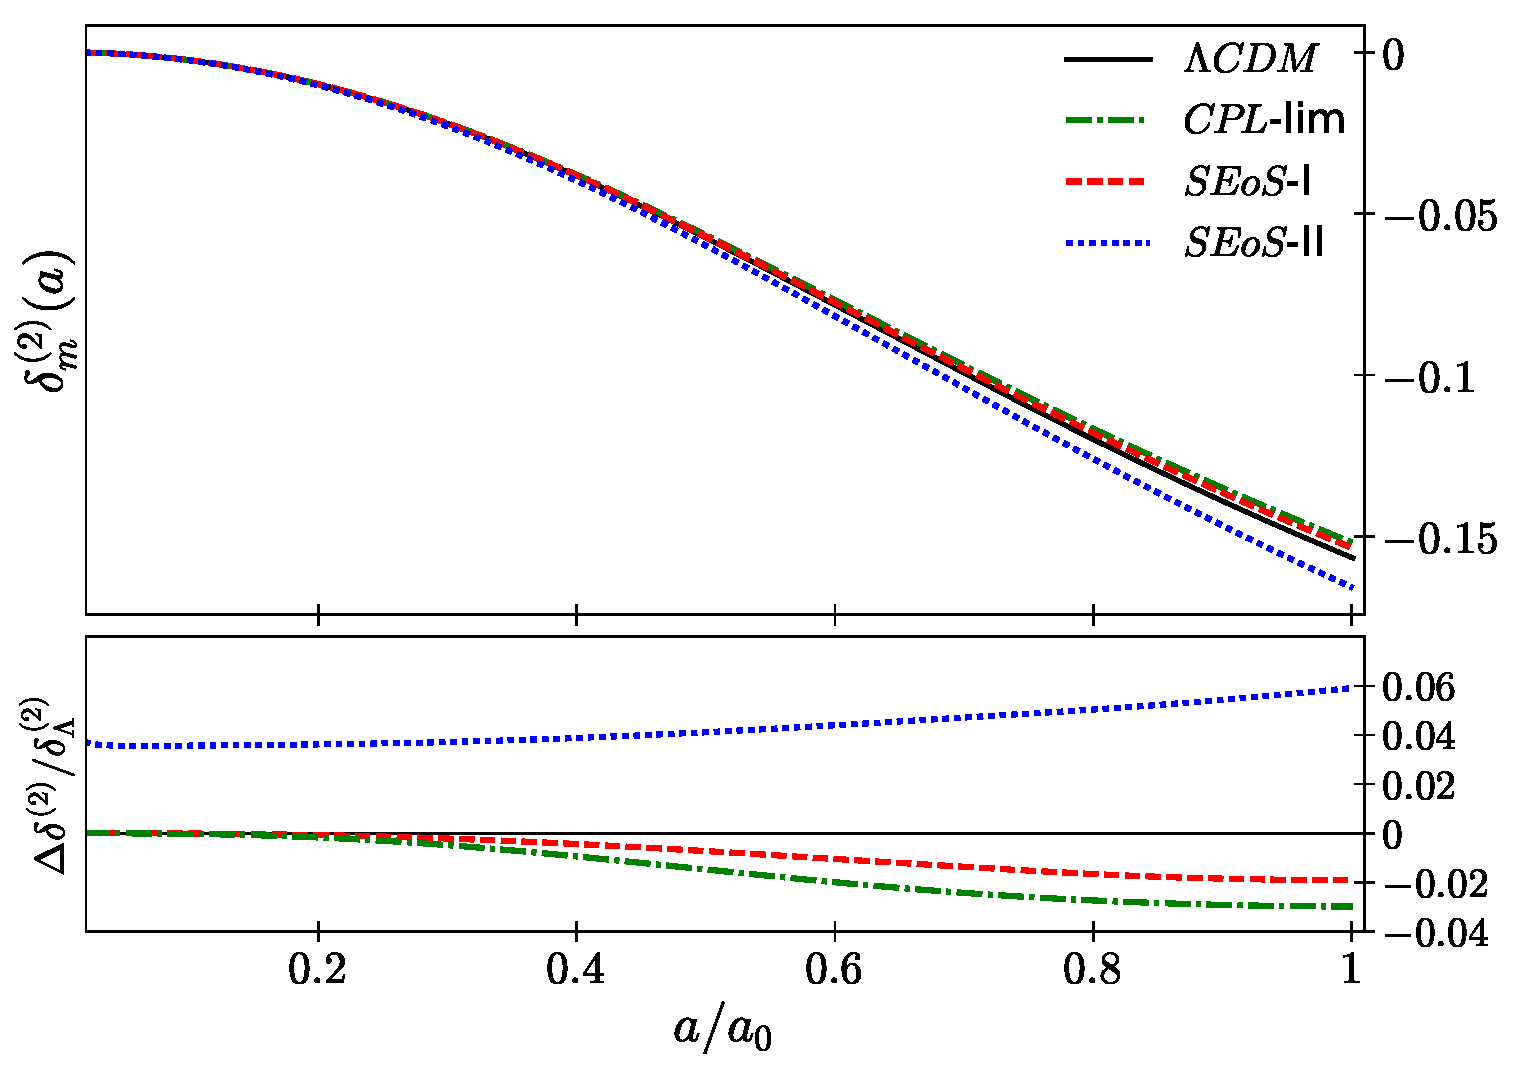
\includegraphics[width=0.49\textwidth,angle=0]{./plots/d2m_4models_ratio_linlin} \\

     \end{tabular}

\caption{%{\it Upper panels:} 
Evolution of the dark matter density contrast at first $\delta_m^{(1)}(a)$ (left panel), and second-order, $\delta_m^{(2)}(a)$ (right panel) for the models considered. The relative differences w.r.t. to $\Lambda$CDM are shown in their respective bottom panels. The case SEoS-I deviates less from $\Lambda$CDM, followed by CPL-lim and SEoS-II. 
}
\label{fig:deltas}
%\end{center}
\end{figure*}

\label{sec:linear}


\begin{figure*}
     \centering
     \begin{tabular}{cc}
        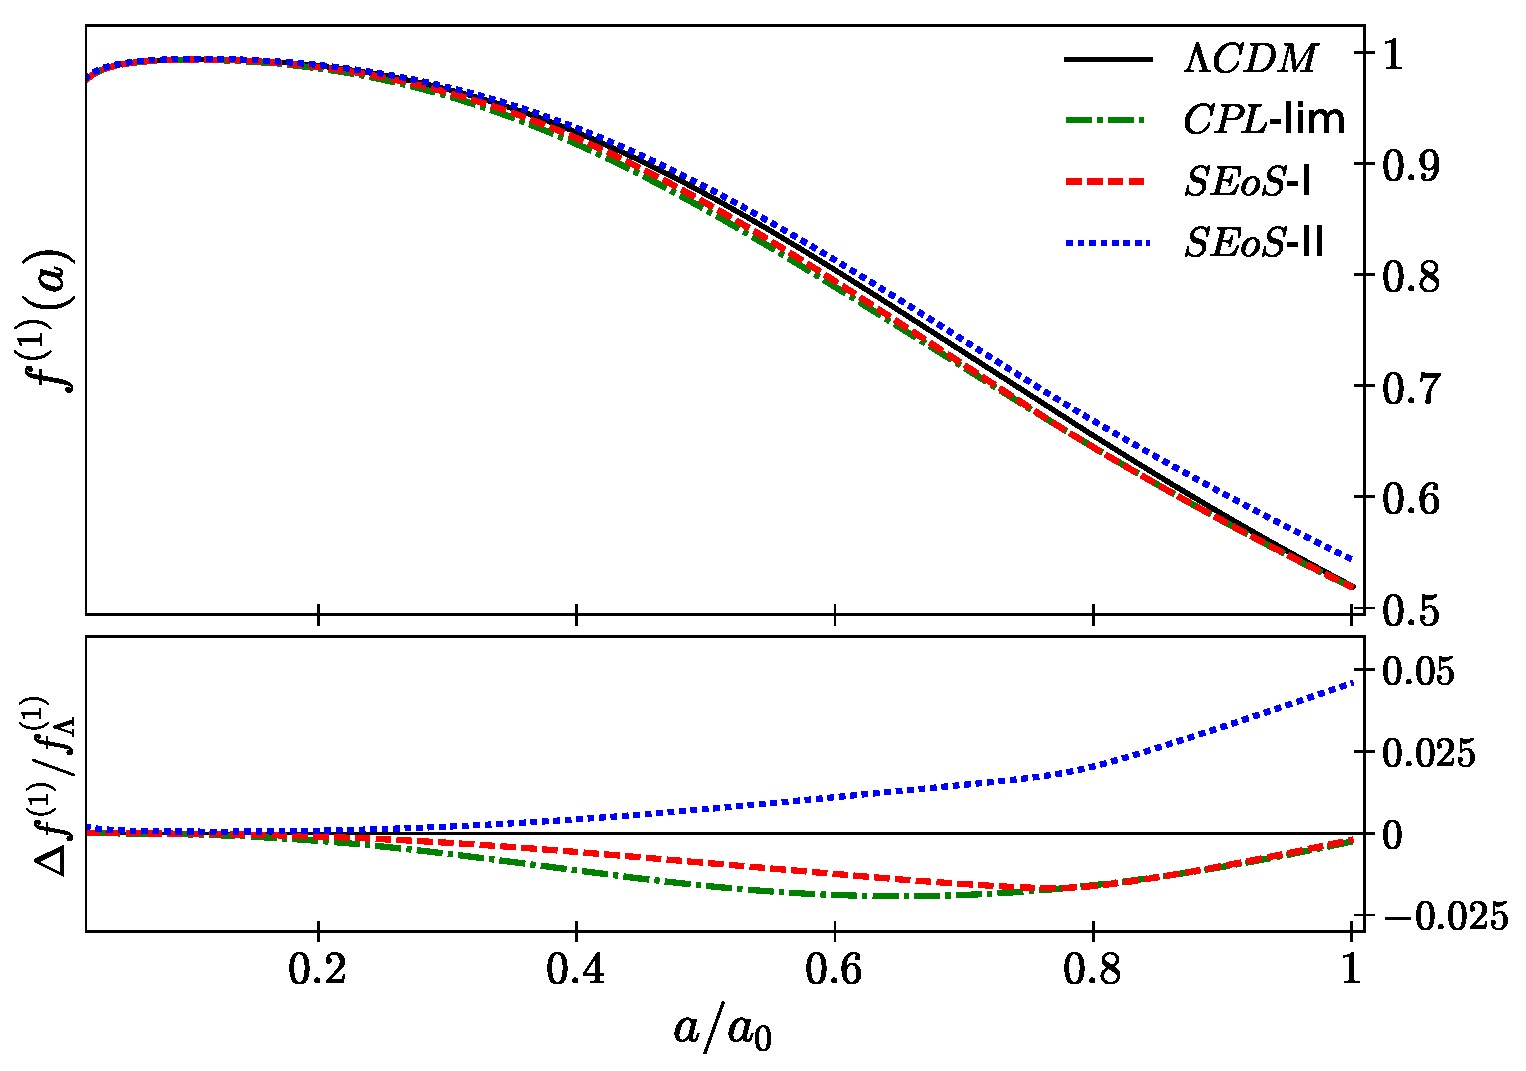
\includegraphics[width=0.5\textwidth,angle=0]{./plots/f1_4models_ratio_linlin}   
        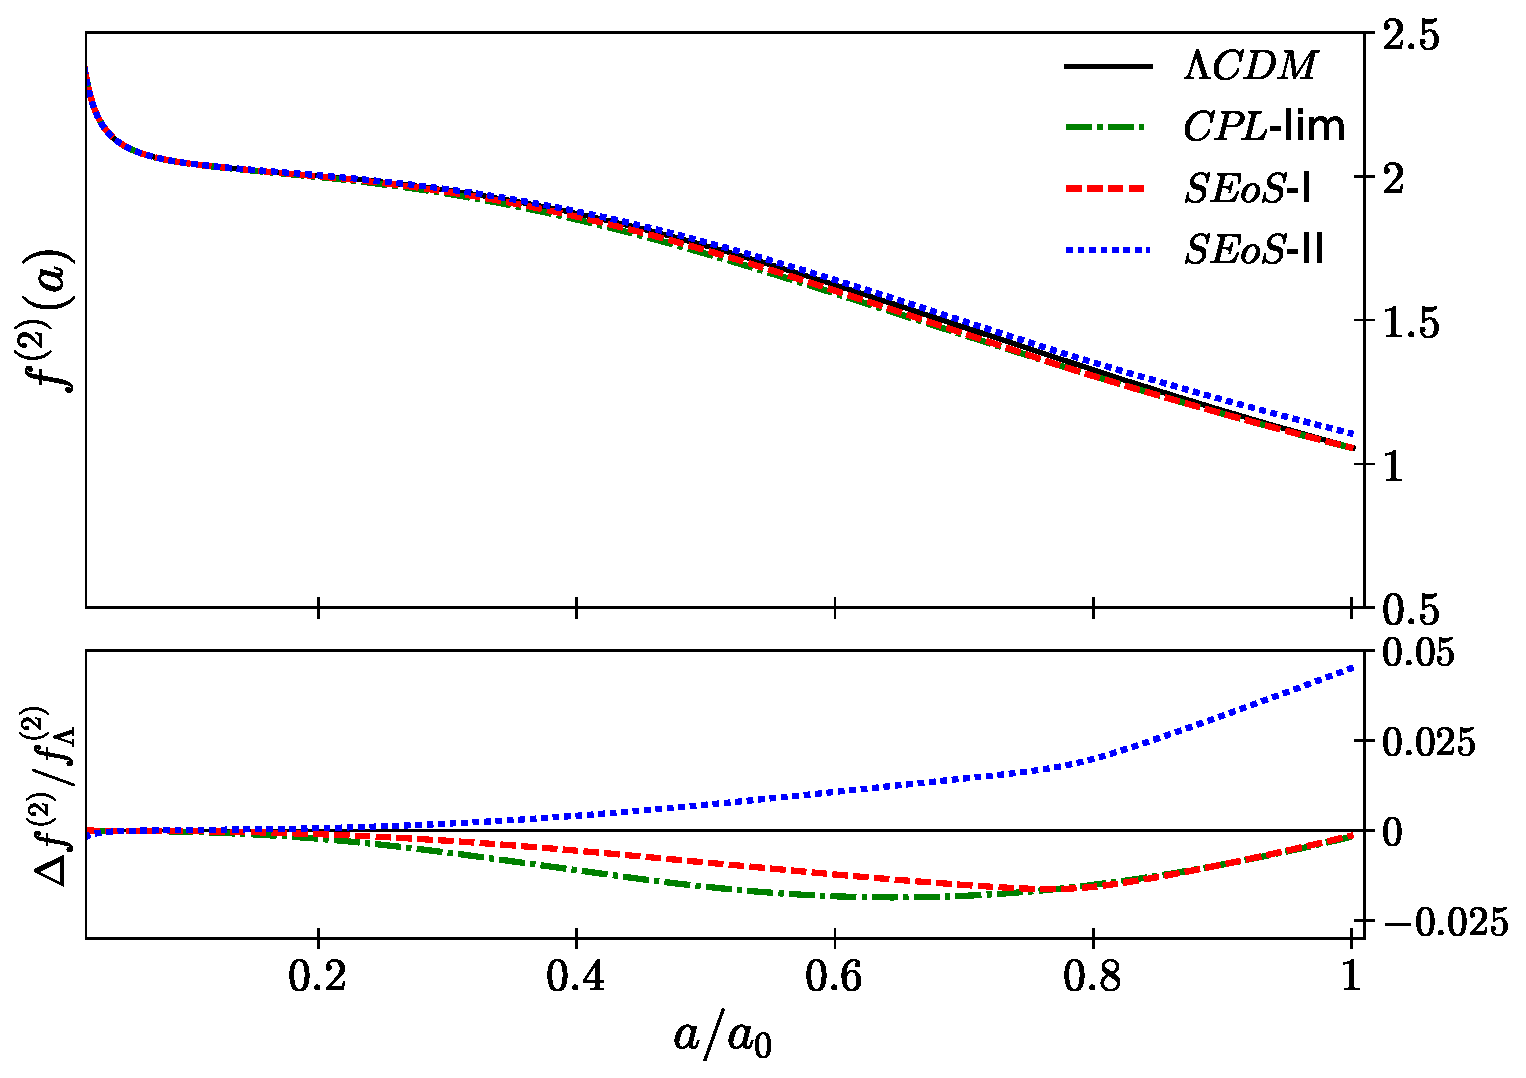
\includegraphics[width=0.5\textwidth,angle=0]{./plots/f2_4models_ratio_linlin} \\

     \end{tabular}

\caption{Evolution of the growth function at first, $f^{(1)}(a)$, and second-order, $f^{(2)}(a)$,  for the models we considered in upper-left and upper-right panels, respectively. The relative differences w.r.t. to $\Lambda$CDM are showing in the bottom panels. The $SEoS$-II model has comparatively higher growth factor in both orders at low redshift, implying faster growing mode then other models. 
}
\label{fig:f_growth}
% \end{center}
\end{figure*}

%%%%%%%%%%%%%%%%%%%%%%%
\subsection{Matter Perturbation Theory}

The evolution of large scale structure is understood to some extent by studying the linear dark matter perturbation theory \cite{Ma:2011nc, Bernardeau:2001qr}. 
Under the assumption that DE remains homogeneously distributed in all scales of our universe, i.e.,  no clustering in the DE component, $\delta \rho_{DE}= 0$, the evolution of the matter density contrast, $\delta_{m} = \frac{\rho_m}{\bar{\rho}_{m}}-1$ up to first and second-order is given by:

\begin{eqnarray}
a^2 \frac{d^2\delta_m^{(1)}}{da^2}+\frac{3}{2}\left(2- w(a)\Omega_{DE}(a)\right)\frac{d\delta_m^{(1)}}{da} -\frac{3}{2}\Omega_m(a)\delta_m^{(1)}(a) = 0,\label{eq:2lptDE1} \\
a^2 \frac{d^2\delta_m^{(2)}}{da^2}+\frac{3}{2}\left(2-w(a)\Omega_{DE}(a)\right)\frac{d\delta_m^{(2)}}{da} -\frac{3}{2}\Omega_m(a)\delta_m^{(2)}(a)= -\frac{3}{2}\Omega_m(a)\left[\delta_m^{(1)}(a)\right]^2 ,
\label{eq:2lptDE2}
\end{eqnarray}
%
where $\Omega_m(a) = \frac{H_{0}^2\Omega_{m0}a^{-3}}{H(a)^2}$ and $\Omega_{DE}(a) =  \frac{H_{0}^2(1-\Omega_{m0})F(a)}{H(a)^2}$. 
%
These coupled differential equations are solved by applying the initial conditions at a time around the recombination epoch, $a_{ini} \approx 0.001$, when the universe was in a matter dominated era, $\Omega_{m} = 1$ (known as ``Einstein-de Sitter'' epoch). In that phase, $\delta^{(1)}_{m}(a)$ evolves linearly with the scale factor and hence we set $\delta_{m}^{(1)}(a_{ini})=a_{ini}$ and  $d\delta_{m}^{(1)}/da(a) = 1$ at $a= a_{ini}$. Likewise, $\delta^{(2)}_{m}(a) \sim -3/7 a^2$ and  $d\delta_{m}^{(2)}/da(a) \sim a $ at $a= a_{ini}$.  


Figure (\ref{fig:deltas}) shows the evolution history of $\delta_{m}^{(1)}$ and $\delta_{m}^{(2)}$ obtained from the above equations. The relative difference w.r.t. $\Lambda$CDM is shown in the respective lower panels.
%
The slight difference in their expansion history, compared to $\Lambda$CDM, makes SEoS-I and CPL-lim models to show lower values in their matter density contrasts w.r.t. $\Lambda$CDM.
%
This is demonstrated in Figure (\ref{fig:deltas}), where we observe a comparatively lower matter density contrasts evolution for both SEoS-I and CPL-lim. For SEoS-I we have differences of $\sim 1\%$ and $\sim 2\%$ in $\delta_{m}^{(1)}$ and $\delta_{m}^{(2)}$, respectively, at $z=0$.% w.r.t. $\Lambda$CDM
% 
The deviation starts to grow around $z \sim 4$ in both cases. In CPL-lim, a deviation reaches to $\sim 1.5\%$ in $\delta_{m}^{(1)}$ and $\sim 3\%$ in $\delta_{m}^{(2)}$ at the same redshift. 
%
However, we do not observe any signatures that can manifest the effect of the steep transition in DE density field in these linear perturbation theory studies. 

In the case of SEoS-II, even though the Hubble expansion rate is higher compared to $\Lambda$CDM, it corresponds to a model with higher matter content, which implies that the DE epoch starts later. Subsequently, the matter density contrast grows faster. % in such scenario.
Therefore, $\delta_{m}^{(1,2)}$  show more significant differences and a faster growth rate over the other cases. 
As expected, the deviation of $\sim 5\%$ is found in $\delta_{m}^{(1,2)}$ at $a = 1$ in SEoS-II. We thus speculate that the possibility of distinguishing between these dynamical DE models from $\Lambda$CDM is around $3-6\%$ via the second-order perturbation theory. %which is qualitatively low while considering the current galaxies surveys precision.

 
To quantify the speed of growth of structure under the cosmological scenarios considered here, we report the logarithmic growth function at first and second order, $f^{(1,2)}\equiv\frac{d\ln\delta_m^{(1,2)}(a)}{d\ln a}$, in Figure \ref{fig:f_growth}. These quantities relate the matter density to velocity dispersion. Figure (\ref{fig:f_growth}) shows that SEoS-I and CPL-lim have comparatively slower growth rates than $\Lambda$CDM in both orders. The growth rate of structures in SEoS-I and CPL-lim models, compared to $\Lambda$CDM, have some specific trends decreasing the rate up to a certain scale and then start to increase until they reach at the same rate as in $\Lambda$CDM. The SEoS-I case turns out to be the closest one to $\Lambda$CDM and SEoS-II has the fastest growing rate over other models. We do expect to observe some effect in the non-linear regime of structure formation as well.

We also fitted $f^{(1,2)}$ for all models using the known fitting formula proposed in \cite{Wang:1998gt} that define $f^{(1,2)}$ as $f^{(1)}=\Omega_m(a)^{\gamma_1}$ and $f^{(2)}= b\times\Omega_m(a)^{\gamma_2}$ with the growth indexes: $\gamma_{1}$, $\gamma_{2}$ and the amplitude parameter, $b$.
The best-fitted values of $\gamma_{1}$, $\gamma_{2}$ and $b$ for all models are listed in table \ref{table:COLA_models}. 
Following \cite{Bouchet1994}, we set $\gamma_1=6/11$, $\gamma_2=0.55$ and $ b=1$ for the $\Lambda$CDM model.

%The accuracy of this fit was examined and found to be within $\sim 0.02\%$ difference between the fitting and numerical values.
%
%Comparing our fitted functions with that of numerically evaluated values from the equations (\ref{eq:2lptDE1}) and (\ref{eq:2lptDE2}), we find a discrepancy of $\sim 0.1 \%$ in $f^{(1)}$, and $f^{(2)}$ solutions, respectively.

%

\section{N-body Simulation: Non-linear Evolution}
\label{sec:nonlinear}

\begin{table*}
	\begin{center}
		\begin{tabular}{l l c c c c c c c c c c}
		%	\hline
		%	\multicolumn{1}{c}{$\La$CDM}\\
			\hline 
			 Model & Alias &$w_0$ & $w_i$ & $q$ & $z_T$ & $\Omega_{m0}$ & $H_0$ & $n_{s}$ &
			 $\gamma_1$ & $b$ & $\gamma_2$ \\
			 \hline \hline 
			$\Lambda CDM$ & $\Lambda CDM$ & -1 & 0 & 0 & 0 & 0.3089 & 67.74 & 0.9667 & 5/9 & 2 & 6/11\\
			\hline
			SEoS  & SEoS-I & -0.92 & -0.99 & 9.98 & 0.28 & 0.3089 & 67.74 & 0.9667 & 0.5527 & 2.0743 & 0.5912\\
			CPL  & CPL lim & -0.92 & -0.99 & 1 & 1 & 0.3089 & 67.74 & 0.9667 & 0.5535 & 2.0751  & 0.5927\\
		\hline
			SEoS & SEoS-II & -0.92 & -0.99 & 9.98 & 0.28 & 0.3340 & 73.22 & 0.9667 & 0.5533 & 2.0859 & 0.5936\\
			\hline %\hline
		\end{tabular}
		\caption{Cosmological and model parameters specification. $\gamma_1$, $\gamma_2$, and $b$, refer to the best fit values found using the fitting formulae for the logarithmic growth functions: $f^{(1)}=\Omega_m^{\gamma_1}$, and $f^{(2)}=b \Omega_m^{\gamma_2}$ \cite{Wang:1998gt}.} 
		\label{table:COLA_models}
	\end{center}
\end{table*}


%____TABLE____________________________________
\begin{table*}
\centering
\begin{tabular}{c|c|c}
\hline
parameter & definition & value \\
\hline
\hline
%$\sigma_{8}$ & r.m.s. linear density fluctuation & $0.8159$ \\
%\hline
$L_{\rm box}$ & simulation box size & 1024~$h^{-1}$Mpc\\
$N_{\rm p}$ & simulation particle number & $1024^3$\\
$N_{\rm Mesh}$ & FFT Mesh & $1024^3$\\
%$m_{\rm p}$ & simulation particle mass & $7.78\times 10^{10}h^{-1}M_{\odot}$\\
$z_{ini}$ & Initial redshift & 49\\
$n_{step}$ & Time steps & 200\\
$ z_{\rm out}$ & Snapshots out at $z$ & $ 0, 0.1, 0.28, 0.56, 1, 1.5, 2, 2.3, 19 $\\
$ N_{\rm run}$ & Number of run & 5 \\
\hline
\end{tabular}
\caption{Specifications of the N-body simulations.}
\label{table:simulation_COLA}
\end{table*}
%____TABLE____________________________________

A way of understanding the structure formation of our Universe in the non-linear regime is by following the formation and distribution of DM halos. This can be done through the full N-body DM simulations. However, in order to achieve a reasonable approximation of the structure formation at large and small scales, the N-body codes need to run numerous time-steps with a fair amount of computational resources.


For our studies we use the COmoving Lagrangian Acceleration (COLA) method\cite{Tassev:2013pn} by modifying the publicly available particle mesh based  N-body code called L-PICOLA\cite{Howlett:2015hfa}. With this N-body DM simulation  we study the cosmological structure formation under the dynamical DE models described in section \ref{sec:background}. 

%we modify the publicly available N-body DM simulation so-called the COmoving Lagrangian Acceleration method\cite{Tassev:2013pn}, particularly L-PICOLA\cite{Howlett:2015hfa} for simulating the cosmological structure formation under the dynamical DE models described in section \ref{sec:background}. 
This scheme has the advantage of accurately recovering the large scale structures (LSS) in few time steps with less usage of computational resources. It is also able to accurately trace the small scales  thanks to the implementation of Lagrangian perturbation theory (LPT), which allows to capture the large scale dynamics directly via the linear growth factors. Note that this makes the code three times faster in comparison to the standard N-body code by enabling it to take larger time steps. 

 
 %This comes from the fact that LSS ($> 100 {\rm Mpc~h^{-1}}$) is well estimated by the Lagrangian perturbation theory. 
 
 %The first and second-order dark matter perturbation solutions are used the COLA code and the small scales are left to be computed by the full N-body method.  
%Due to the fact that the large scale structures ($> 100 {\rm Mpc~h^{-1}}$) can be estimated well by the Lagrangian perturbation theory,  the first and second-order dark matter perturbation solutions are being used in the COLA code and the small scales are left to be computed by the full N-body method. 
%This makes the code 3 times faster in comparison to the standard N-body codes by enabling it to take larger time steps. 
In the following subsection, we briefly describe the COLA method and the Lagrangian perturbation theory employed in the code.

%Basically, in the N-body simulation, the time integration for the large scales is done by solving the linear growth factor but with a few time-steps with an N-body code will provide a wrong clustering for the large-scale.
%For more details we refer to \cite{Tassev:2013pn} and references therein.
%\subsection{2LPT METHOD}

\subsection{COLA Method}

%Previous study has shown that different models predict the differences mainly on small scales ($r < 1 h^{-1}Mpc$) which arguing that an accurate clustering measurements on the small scales can provide significant constraints on the Dark energy or modified gravity models. 

The cold dark matter N-body simulations are governed by a system of equations conformed by the equation of motion and the Poisson equation:
\begin{equation}
\frac{d^2 {\bf x}}{d\tau^2} = - {\bf \nabla} \Phi_{N},
\label{eq:geodesic}
\end{equation}
\begin{equation}
\nabla^2\Phi_{N} = 4 \pi G {\bar{\rho}_{m}}a^4 \delta_{m},   
\label{eq:poisson1}
\end{equation}
where $d\tau = \frac{dt}{a}$ represent the conformal time, $\delta_{m}=\frac{\rho_{m}}{\bar{\rho}_{m}}-1$, the  matter density contrast in the particle positions $\bf{x}$, and $\Phi_N$ is the Newtonian potential.

However, in the COLA approach rather then solving the Newtonian potential for the particle positions, $\vec{x}$, one solves for the perturbation around the path $\vec{x}_{LPT}$ provided by the second-order Lagrangian perturbation theory, i.e., $\vec{x} = \vec{\delta x}+\vec{x}_{LPT}$. Thus, the equation of motion takes the form:
\begin{equation}
\frac{d^2 \vec{\delta x}}{d\tau^2} = - \vec{\nabla} \Phi_{N} - \frac{d^2\vec{x}_{LPT}}{d\tau^2}.
\end{equation}
This equation is solved as a system of coupled equations: 
\begin{equation}
\frac{d\vec{\delta}v}{d\tau} = -\vec{\nabla}\Phi_{N} - \frac{d^2\vec{x}_{LPT}}{d\tau^2},
\end{equation}
\begin{equation}
\frac{d\vec{\delta x}}{d\tau} = \vec{\delta v},   
\end{equation}
which will track the large scale evolution according to the Lagrangian perturbation theory.
\subsubsection{2LPT}
According to the Lagrangian perturbation theory (LPT) \cite{Bernardeau:2001qr}, the position of a particle in Eulerian space, $\bf{x}$, is described by its initial Lagrangian position, $\bf{q}$, and a displacement field of the particle, $\bf{\Psi}$, through the mapping:  
\begin{equation}
\bf{x}(q,\tau) = \bf{q}+\bf{\Psi}(\bf{q},\tau),
\label{eq:LPT_position}
\end{equation}
and the equation of motion \eqref{eq:geodesic} as given by
\begin{equation}
\frac{d^2 \bf{\Psi}}{d\tau^2} + \mathcal{H}(\tau)\frac{d\bf{\Psi}}{d\tau} +{\bf \nabla}\Phi_N = 0.
\label{eq:geodesic2}
\end{equation}
Hence, the Poisson equation \eqref{eq:poisson1} can be written as
\begin{equation}
{\bf \nabla_{x}} \left( \frac{d^2 \bf{\Psi}}{d\tau} + \mathcal{H}(\tau)\frac{d\bf{\Psi}}{d\tau}\right) = \nabla^2\Phi_N = - \frac{3}{2}\Omega_{m0}\mathcal{H}(\tau) \delta_{m}(\tau)= -\kappa \delta_{m},
\label{eq:poisson}
\end{equation}
where $\kappa = \frac{3}{2}\Omega_{m0}\mathcal{H}(\tau)$, and $\mathcal{H}$ is the conformal Hubble expansion rate. 

In LPT, the above equation is generally solved by perturbatively expanding the displacement vector as $\bf{\Psi} = \bf{\Psi}^{(1)} +\bf{\Psi}^{(2)}+ ...$, where $\bf{\Psi}$ represents a curl-free gradient of a scalar field, $\phi^{(i)}$, $\bf{\Psi}^{(i)} = \bf{\nabla}_{q}\phi^{(i)}$.
Similarly, expanding the density contrast in a perturbative series we have $\delta_m(x) = \delta_m^{(1)}+ \delta_m^{(2)}+ ... = J^{-1}-1$, with $J = \rm{Det}(\delta_{ij} +{\bf{\Psi}}_{i,j})$, the Jacobian of the transformation. Now  we can equate each order and obtain:
%$\delta = \delta^{(1)}+ \delta^{(2)}+ ... = \left|\frac{\partial(x)}{\partial(q)}\right|^{-1} - 1 = J^{-1}-1$
\begin{equation}
\delta_{m}^{(1)} = - \bf{\Psi}^{(1)}_{i,i},
\end{equation}
\begin{equation}
\delta_{m}^{(2)} = - \bf{\Psi}^{(2)}_{i,i} +\frac{1}{2}\left((\bf{\Psi}^{(1)}_{i,i})^2 +(\bf{\Psi}^{(1)}_{i,j})^2\right),
\label{eq:delta2}
\end{equation}
where $\bf{\Psi}_{i,j}=\partial \bf{\Psi}_{i}/\partial q_{j}$, and the divergence w.r.t. $x$ is changed to $q$ via the Jacobian transformation: $\nabla_{x_i} =(\delta_{ij}+{\bf{\Psi}}_{i,j})^{-1}\nabla_{\bf q_j}$. 
At first order, we have from equation \eqref{eq:poisson}:
\begin{equation}
\frac{d^2 {\bf\Psi}^{(1)}_{i,i}({\bf q},\tau)}{d\tau^2} = -\kappa \delta_{m}^{(1)}({\bf q},\tau),    
\end{equation}
which is equivalent to 
\begin{equation}
\left(\frac{d^2}{d\tau^2}-\kappa\right) \nabla^2 \phi^{(1)}({\bf q},\tau) =0,
\label{eq:1st_LPT}
\end{equation}
%
where $\phi^{(1)}({\bf q},\tau)$ is factorized into the time-dependent normalized growth factor, $D^{(1)}(\tau)$ multiplied by $\phi^{(1)}({\bf q},\tau_{in})$, the initial condition field coming from $\delta^{(1)}({\bf q},\tau_{in})$. Thus, the growth factor $D^{(1)}(\tau)$ follows the equation:
\begin{equation}
\left(\frac{d^2}{d\tau^2}-\kappa\right) D^{(1)} =0,
\end{equation}
%
and it can  be solved easily by assuming the initial conditions according to the growing mode of the matter dominated ``Einstein de-Sitter'' Universe, $D_{in}^{(1)} =1$, and $\frac{dD^{(1)}_{in}}{d\tau}=\left(\frac{1}{a}\frac{da}{d\tau}\right)_{\tau =\tau_{in}}$. 

Note that it is the same solution we obtained from eq. \eqref{eq:2lptDE1}.  
So, the first-order displacement field at any time is simply given by ${\bf \Psi}^{(1)}(q,\tau)= D^{(1)}(\tau){\bf \Psi}^{(1)}(q,\tau_{i})$, i.e., once the displacement field at the initial time is computed in the simulation,  $\bf{\Psi}^{(1)}$, we can track it at any later time simply multiplying it by the growth factor.
Similarly, using the equations \eqref{eq:delta2} and \eqref{eq:poisson}, the second-order Lagrangian perturbation takes the form of 
\begin{equation}
\left(\frac{d^2}{d\tau^2} -  \kappa \right)\nabla^2\phi^{(2)} = -\frac{\kappa}{2}\left[(\nabla^2\phi^{(1)})^2 - (\nabla_{i}\nabla_{j}\phi^{(1)})^2\right],
\label{eq:2nd_LPT}
\end{equation}
with $\phi^{(2)}(q,\tau) = D^{(2)}(\tau)\phi^{(2)}(q,\tau_{in})$, and where the second-order growth factor $D^{(2)}$ satisfies 
\begin{equation}
\frac{d^2 D^{(2)}}{d\tau^2}-\kappa D^{(2)} = -\kappa (D^{(1)})^2.
\label{eq:D2}
\end{equation}
%
We again provide the initial conditions according to an Einstein-de Sitter Universe: $D^{(2)}_{in} = -\frac{3}{7}$ and $\frac{dD_{in}^{(2)}}{d\tau} = - \frac{6}{7}\left(\frac{1}{a}\frac{da}{d\tau}\right)_{in}$, and the solution is nothing but the solution of \eqref{eq:2lptDE2}. The second-order initial field, $\phi^{(2)}(q,\tau_{in})$, is given by
 \begin{equation}
\nabla^{2}\phi^{(2)} = \frac{1}{2}\left[(\nabla^2\phi^{(1)})^2 - (\nabla_{i}\nabla_{j}\phi^{(1)})^2\right]. 
 \end{equation}
Hence, in LPT, the equation \eqref{eq:LPT_position} reduces to 
\begin{equation}
{\bf x} = {\bf q}- D^{(1)}{\bf\nabla_{q}}\phi^{(1)}+D^{(2)}{\bf \nabla_q}\phi^{(2)}, 
\label{eq:LPT_position_pot}
\end{equation}
and the velocity field, $v$ is governed by
\begin{equation}
{\bf v} =\frac{d{\bf x}}{d\tau} = -D^{(1)}f^{(1)}\mathcal{H} {\bf \nabla_{q}}\phi^{(1)}+D^{(2)}f^{(2)}\mathcal{H}{\bf \nabla_{q}}\phi^{(2)},
\end{equation}
where $f^{(1,2)}$ represent the growth rate functions $f^{(1,2)} = \frac{d\ln D^{(1,2)}}{d\ln a}$.

For our dynamical DE models, $D^{(1,2)}$ and $f^{(1,2)}$ are provided by solving equations \eqref{eq:2lptDE1} and \eqref{eq:2lptDE2} along with their Hubble expansion rates. The main differences observed among each other and from $\Lambda$CDM have been discussed in subsection (\ref{sec:linear}).

%From Figure \ref{fig:hubble_ratios} we observe that the difference in Hubble rates for the $CPL$-lim and $SEoS$-I models from the $\Lambda CDM$ remain within $\sim 2\%$ throughout all redshifts.    In case of $SEoS$-II model, the deviation reaches up to $\sim 12\%$ starting from the $z=1$ towards higher redshifts.

\subsubsection{COLA Approach}
In the COLA method, the equation of motion is solved in the frame of reference comoving with the particles in Lagrangian space.  
%
After the method is applied, we have the residual displacement, $\Psi_{res}$, where the Zel'dovich and quasi-linear 2LPT displacement fields ($\Psi^{(1)}$ and $\Psi^{(2)}$, respectively) have been subtracted from the full non-linear displacement that each particle experiences.

\begin{equation}
\Psi_{res} = \Psi - D^{(1)}\Psi^{(1)} - D^{(2)}\Psi^{(2)}.    
\end{equation}
Hence, the equation of motion(\ref{eq:geodesic2}) takes the form:
\begin{equation}
T^2[\Psi_{res}] = -\nabla\Phi_{N}- T^2[D^{(1)}]\Psi^{(1)} - T^2[D^{(2)}]\Psi^{(2)} 
\end{equation}
where $T^2[X] = \frac{d^2X}{d\tau^2} +\mathcal{H}\frac{dX}{d\tau}$. The residual displacement, $\Psi_{res}$ is left  to be computed by the usual Particle-Mesh scheme.

For more details about the method implementation and the way the time integration has been discretized on the operator, $T$, we refer the reader to references \cite{Tassev:2015mia, Howlett:2015hfa}. 
%
Note that in the limit of a large number of time-steps, this method recovers the same result as the standard approach for N-body simulations both on the large and small scales.

Thus, in the COLA approach, the run time is directly proportional to the number of time steps we set to run the simulation. Previous studies of the COLA approach have already shown that with ten steps, it converges to the same results as a full-N body simulation with an accuracy of up to $2\%$ for $k = 1h/Mpc$. Hence the convergence rate increases as we increase the number of time steps. Nevertheless, we recall that the goal of our work is not to test the accuracy of the code, but rather to study the effect of dynamical DE models.


%The mass of the particle is determined by 
%$m_{particles} = \frac{\Omega_{m0}\times\rho_{crit}* L^3}{N_{particles}} $

\subsection{Simulation set up}

We follow Planck cosmology \cite{Ade2016}: $\Omega_{m0}=0. 3089$, $h =0.6774$, $n_s=0.9667$, $\sigma_8=0.8159$, and the model parameters are set according to the best fit values from \cite{Jaber:2017bpx}. Specifically, for the CPL-lim we have $w_{0} = -0.92, w_{i} =-0.99, z_{T} =1 =q$ and the SEoS models have $w_{0} =-0.92, w_{i} =-0.99, z_{T}=0.28, q=9.98$. We recall that SEoS-I and SEoS-II models are differentiated by the fact that SEoS-II is run with $\Omega_{m0}=0.334$ and $ h=0.7322$. 

For the N-body simulations we use a box of side length $L_{\rm box}=1024 h^{-1}{\rm Mpc}$ (L1024 in Table \ref{table:simulation_COLA}), $N_{p} = 1024^3$ dark matter particles, and a mesh of $N_{\rm mesh}= 1024$ for FFT calculations.
%The parameters for the N-body simulations are box size $L_{\rm box}=1024 h^{-1}{\rm Mpc}$ (L1024) with $N_{p} = 1024^3$ dark matter particles on a mesh, $N_{\rm mesh}= 1024$. 
These parameters lead to a value for the mass of particles: $m_{part}=8.57198 \times 10^{10}{\rm M_{\odot}}h^{-1}$ for $\Omega_{m0}=0.3089$, and $m_{part}=9.2685 \times 10^{10} {\rm M_{\odot}}h^{-1}$ for $\Omega_{m0} = 0.334$, respectively. 


The initial matter power spectra that we input to the simulations was generated with \texttt{CAMB}\footnote{https://camb.info/}. The initial particles distribution is created using the 2LPTic initial conditions code \cite{Crocce:2006ve} \footnote{http://cosmo.nyu.edu/roman/2LPT/} at the initial redshift of $z_{in}=49$. 
%
Upon the modification of the COLA-code by incorporating the behavior of dynamical DE models, we run the simulation with 200 time-steps between  $z_{in}=49$ and $z=0$, and take several snapshots at different redshift values for each model. To suppress sampling variance on our results, we estimate them by averaging 5 independent realizations, each one run with different random seeds. Our results will be focused at redshifts, $z=0, 0.28 $ and $1$. Keeping in mind that $z=0.28$ and $z = 1$ are the transition points, $z_{T}$, for SEoS models and CPL-lim respectively. 
A summary of the cosmological and simulation parameters is listed in tables (\ref{table:COLA_models}) and (\ref{table:simulation_COLA}). 

\section{Results}
\label{sec:results}
The effect of dynamical dark energy is often studied through the dark matter particles and halo properties. 
Particularly through quantities such as the dark matter power spectrum, velocity power spectrum, halo abundances and halo-clustering at different redshifts. 
For our case, we calculate the matter power spectrum using the SimplePofk code \footnote{http://ascl.net/1110.017} \cite{Colombi2011}, where the density field is estimated using a Cloud-in-Cell mass assignment method on a cubic grid with the same resolution as the Particle-Mesh grid used for the integration of the N-body system. 
The halo catalogs are generated using a publicly available phase-space temporal halo finder called Rockstar \footnote{https://bitbucket.org/gfcstanford/rockstar} \cite{Behroozi2013}. The Rockstar halo-finder is set to find  the halos with a minimum of $20$ particles, which leads to the minimum mass of the halo of $\sim 2 \times 10^{12}{M_{\odot}}h^{-1}$. Later on, we study the effect on the dark matter halos clustering by calculating the two-point correlation function in real space. 
%For this propose we use a publicly available code called CUTE \cite{cutecode}\footnote{https://github.com/damonge/CUTE}. 

\subsection{Non-linear matter power-spectrum} 

\begin{figure*}
     \centering
     \begin{tabular}{cc}
        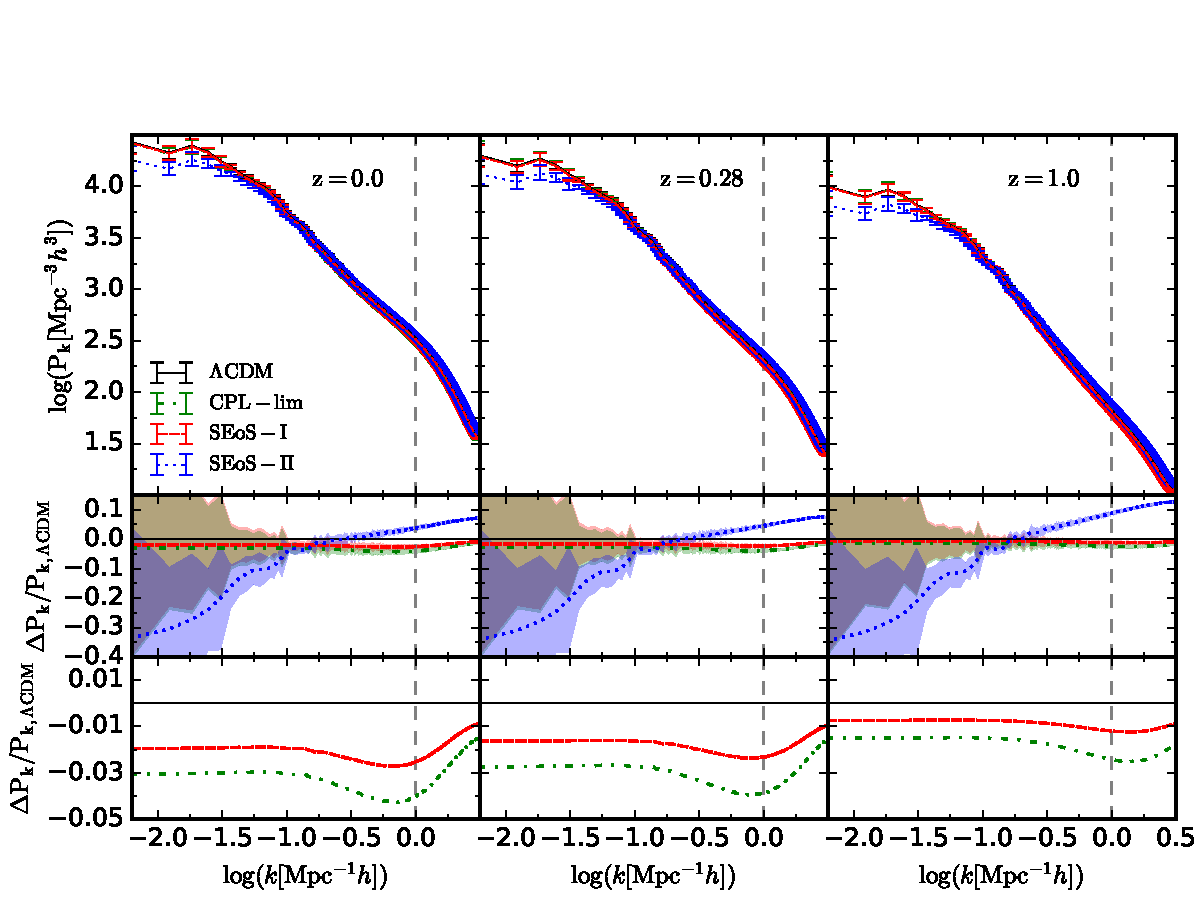
\includegraphics[width=1\textwidth,angle=0]{./plots/power_spectrum_all.pdf}   

 \end{tabular}

\caption{{\it Upper Panels:} The dark matter power spectra for all the models at redshifts: $z = 0, 0.28, 1$. We follow the same color coding to represent the corresponding models as before. {\it Middle panels}: The relative difference of our models w.r.t. $\Lambda$CDM. Shaded regions represent one sigma standard deviation propagated from 5 realizations run with the different random seeds. {\it Lower panels}: Relative differences of SEoS-I and CPL-lim w.r.t. $\Lambda$CDM. The vertical line provides the limit beyond which the $P_{k}$ can not be trusted. 
%Note: The SEoS-I and CPL models show difference less then $\sim 3-4\%$ from $\Lambda$CDM.
}
\label{fig:pk_nonlinear}
%\end{center}
\end{figure*}



\label{sec:pk} 

In Figure (\ref{fig:pk_nonlinear}), the non-linear matter power spectra, $P_{k}(k,z)$ of all models are plotted at  redshifts $z=0$, $0.28 $, and $1.0$. The power spectra are based on the simulation ${\rm L1024}$. In each panel, solid black, green dotted-dash, red dashed, and blue dotted lines correspond to $\Lambda$CDM, SEoS-I, CPL-lim, and SEoS-II models, respectively. The relative differences w.r.t. $\Lambda$CDM for all models are shown in the middle panels. The shaded portions represent the error propagated from the $1\sigma$ standard deviations of 5 realizations, run with the different initial random seeds. The bottom panels highlight the difference between SEoS-I, and CPL-lim from $\Lambda$CDM.  

%Figure (\ref{fig:pk_nonlinear}) show a consistent standard behavior of $P_{k}$ of all models with the variation of redshift.% i.e., $P_{k}$ reduces with the increase of redshift. 
 %From the bottom panels of Figure (\ref{fig:pk_nonlinear}),
The $P_{k}$ of SEoS-I (red dashed) and CPL-lim (blue dotted) show a deficit in power of $\sim 2\%$ and $\sim 3\%$, respectively, throughout all k-scales w.r.t. $\Lambda$CDM, and a slight increase in power at the non-linear regimes that reaches $\sim 3-4\%$ (see bottom panels of Figure (\ref{fig:pk_nonlinear})). Note that the maximum deviation observed in the linear growth $\delta^{(1,2)}$ for these models is within $\sim 2-3\%$ at $z = 0, 0.28, 1$. This points out that the impact of dynamical DE is relatively small both in linear and non-linear regimes.

However, the overall deficits in $P_{k}$ for SEoS-I and CPL-lim highlight the impact that different DE dynamics has in the growth of structure. Explicitly, the effect of having less negative values of $w(z)$ for both SEoS-I and CPL-lim compared to $\Lambda$CDM (for instance: $w_{SEoS-I} =  -0.97$, $w_{CPL-lim} = -0.95$ and $w_{\Lambda}= -1$ at $z = 0.28$), makes the models to evolve with a slightly larger expansion rate, $H(a)$, and therefore to enter the DE-dominated epoch relatively earlier than in $\Lambda$CDM. This results in slowing down the growth of structures as compared to a $\Lambda$CDM universe. 

The trend of a reduction in the  $P_{k}$ amplitude as redshift goes to zero is again showing the effect of DE behavior, as a consequence of their expansion rates. In particular, $2 \%$ and $3 \%$ differences at $z = 0$ reduce to $1 \%$ and $2 \%$ at $z = 1.0$ for SEoS-I and CPL-lim, respectively.

On the other hand, the $P(k)$ of SEoS-II can be understood by recalling the behavior of linear power spectrum, $P_{k,lin}$, of $\Lambda$CDM  for varying $\Omega_{m0}$ and $H_{0}$. For instance, looking at $P_{k,lin}$ of $\Lambda$CDM at $\Omega_{m0} =0.3089$ and $\Omega_{m0}=0.334$ for the same $H_{0}$, we find that $P_{k,lin}$ of $\Omega_{m0}=0.334$ has a deficit in power at low $k$-modes (linear regime), then it increases and peaks in amplitude at high $k$-modes (non-linear regime). The larger the value of $\Omega_{m0}$, the greater deviation we observe in $P_{k,lin}$, depicting the direct proportionality of $P(k)$ with $\Omega_{m0}$ both in linear and non-linear regimes (see Figure \ref{app:Pk_initial}).
Since $H_{0}$ does not change with time, the difference in $P_{k}$ at different redshifts are not effected by $H_{0}$.
%The deviation can go from $\sim 10\%$ deficit in power at $k = 0.001$ upto $\sim 20\%$ enhancement at $k =10$, noting the difference of $8\%$ in $\Omega_{m0}$ (see Figure \ref{app:Pk_initial}). Larger the value of $\Omega_{m0}$, higher the deviation we observed in $P_{k,lin}$, showing the direct proportionality to $\Omega_{m0}$ both in linear and non-linear regimes with the shift in $P_{k}$. % The effect of having a larger value of $H_{0} = 0.7332$ on the $P_{k}$ is more predominant in the non-linear regime. Higher $H_{0}$, larger the deviation we observed in $P_{k}$ when compare with $H_{0} = 0.6774$.  


Even though the effect of DE is manifested in a greater proportion in the linear regime for models SEoS-I and CPL-lim, for SEoS-II we have the conjunction of DE dynamics with the larger value of the amount of matter contained, $\Omega_{m0} = 0.334$. For this large value of $\Omega_{m0}$, the structures formed in denser environments (see $\delta^{(1,2)}$ in Figure (\ref{fig:deltas})), which subsequently led to low values in $P_{k}$ at low $k$-modes. 

%Even though the effect of DE in general is larger at the linear regime over the non-linear one, in case of SEoS-II where the matter contained, $\Omega_{m0} = 0.334$ is much higher then other models including $\Lambda$CDM, i.e., $\Omega_{m0} = 0.3089$, the structures formed in such environments are more dense (see $\delta^{(1,2)}$ in Figure (\ref{fig:deltas})), thus, subsequently leads to low values in $P_{k}$ at low $k$ modes. 
%

Having the values $\Omega_{m0} = 0.334$ and $H_{0} = 0.7332$ results in more clustering at the non-linear regimes. More specifically, our result in Figure (\ref{fig:pk_nonlinear}) shows a difference as large as $\sim 30\%$ at $k= 0.001$ between the SEoS-II model and $\Lambda$CDM, difference that reduces up to $\sim 10\%$ at the non-linear regime (say $k=10$). The slight reduction in power of $P_{k}$ of SEoS-II between $z = 1$ and $z = 0$ on high $k$-modes is due to DE effect that we observe in $H(a)$ (see Figure (\ref{figure:hubble})).


From this analysis we find that the effect of having a steep transition in the DE models does not imprint a sharp signature in the  $P_{k}$, but does affect it due to the overall impact  of DE dynamics.
%is difficult to detect in $P_{k}$ in front of overall impact  of DE.
As expected from the background studies, SEOS-I turns out to be the closest to $\Lambda$CDM, followed by CPL-lim and SEoS-II



\subsection{Two point correlation function}

\begin{figure*}
	\centering
	\begin{tabular}{cc}
		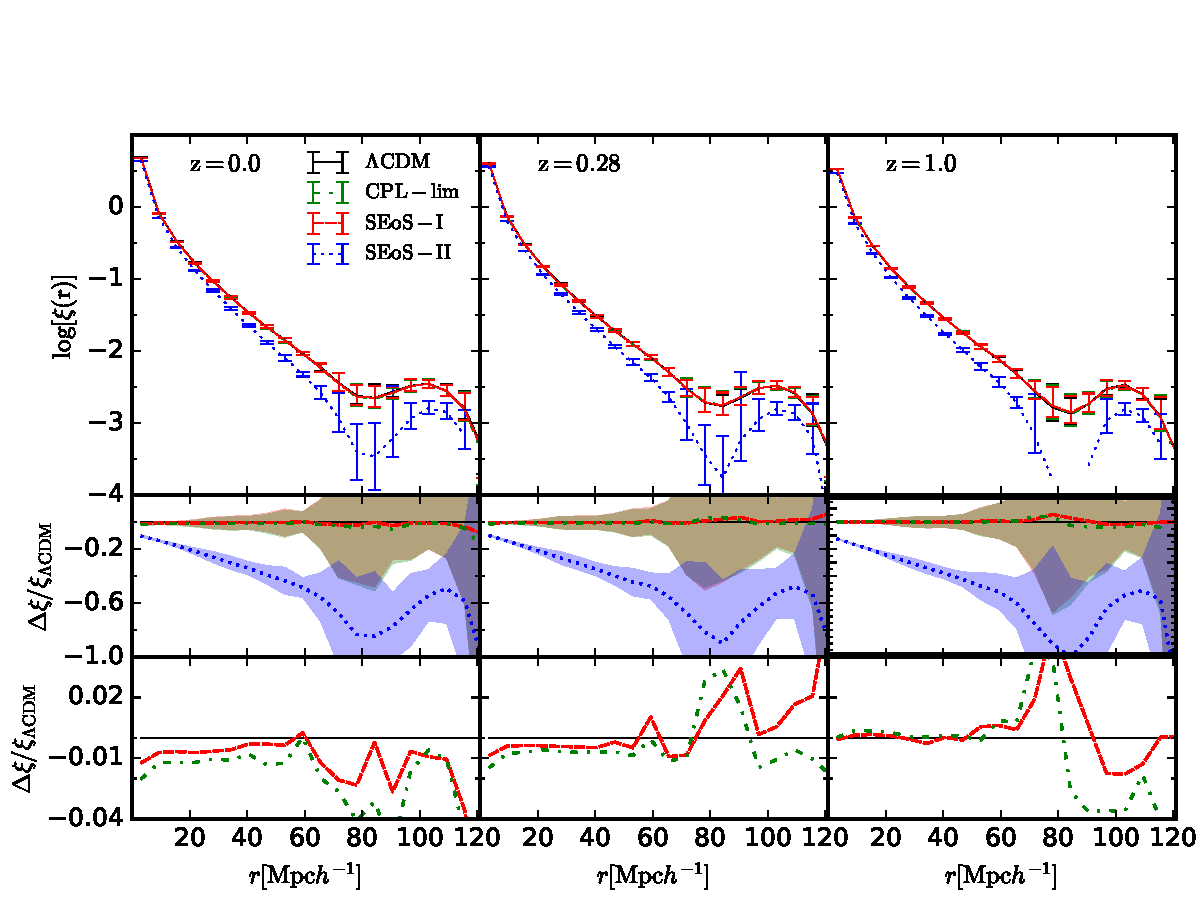
\includegraphics[width=1\textwidth,angle=0]{./plots/2cpf_new.pdf}
		%  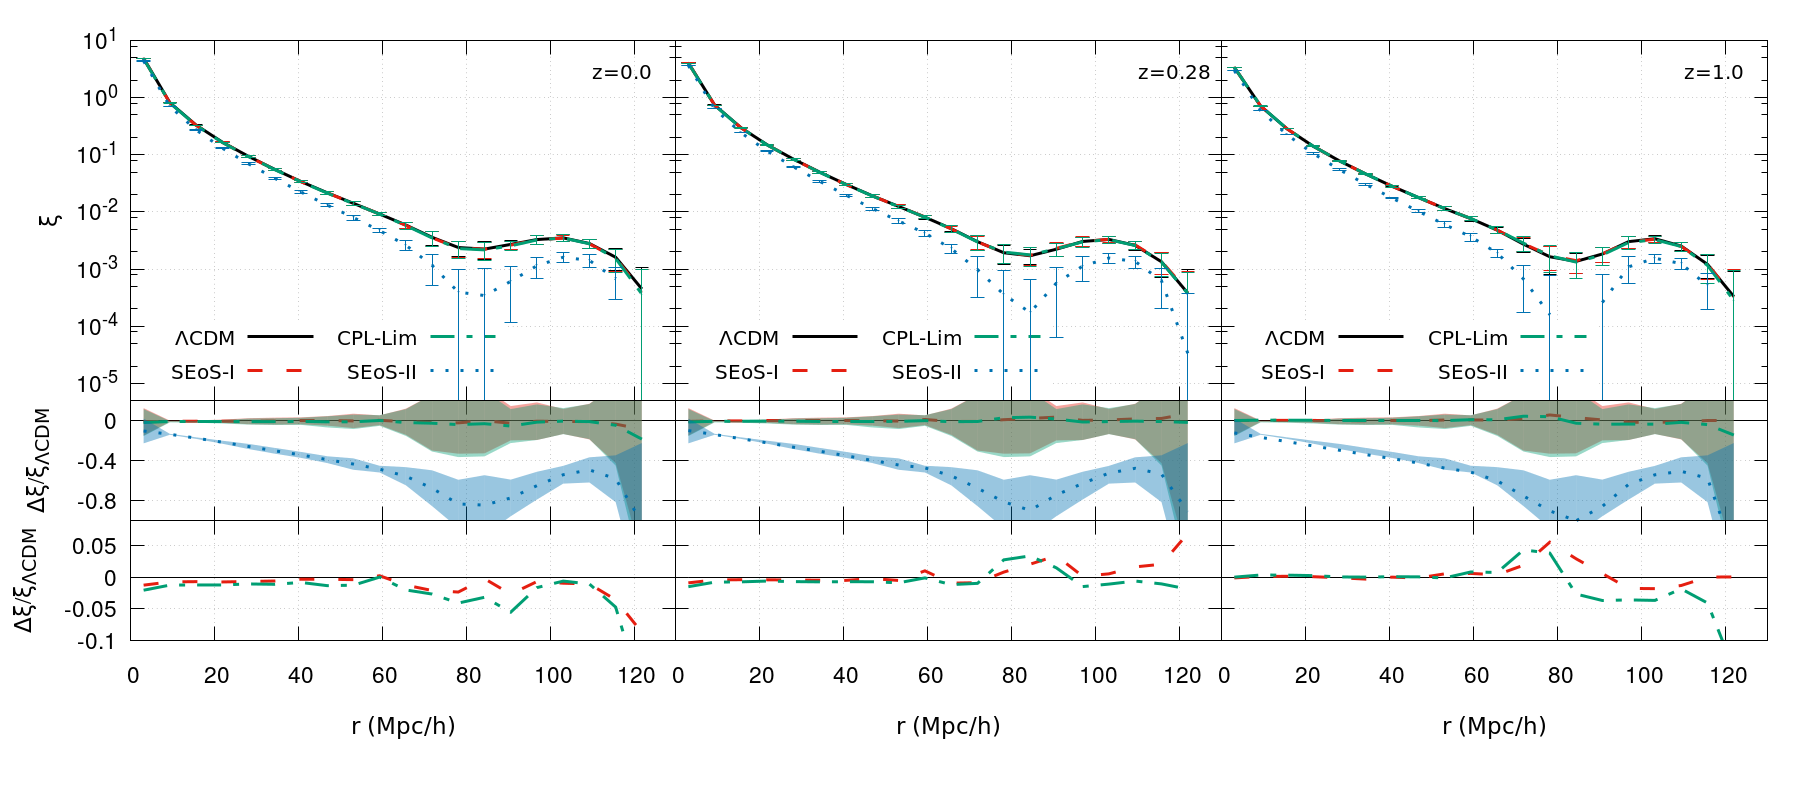
\includegraphics[width=1\textwidth,angle=0]{./plots/HS-50_Prom_2PCF_wZoom_sinr2_halos_Lb1024_}
		%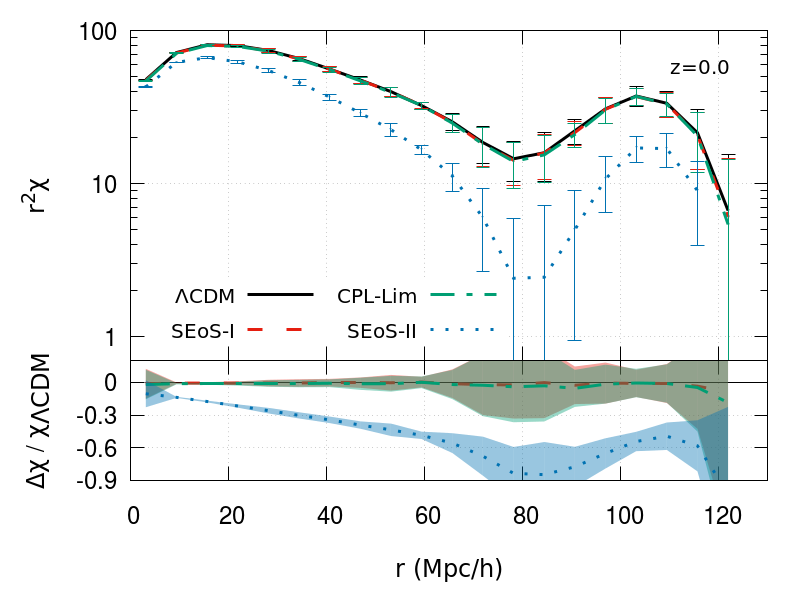
\includegraphics[width=0.33\textwidth,angle=0]{./plots/HS-50_Prom_2PCF_halos_Lb1024_out11}   
		%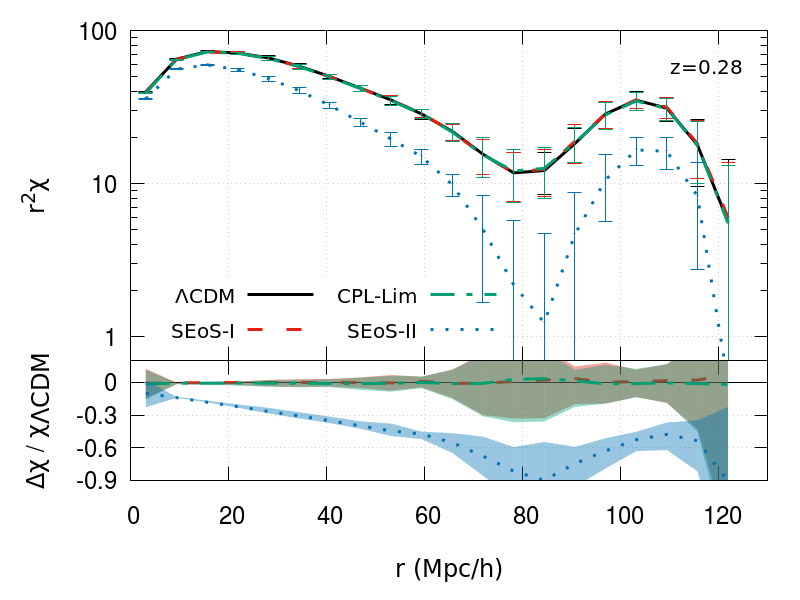
\includegraphics[width=0.33\textwidth,angle=0]{./plots/HS-50_Prom_2PCF_halos_Lb1024_out9} 
		% 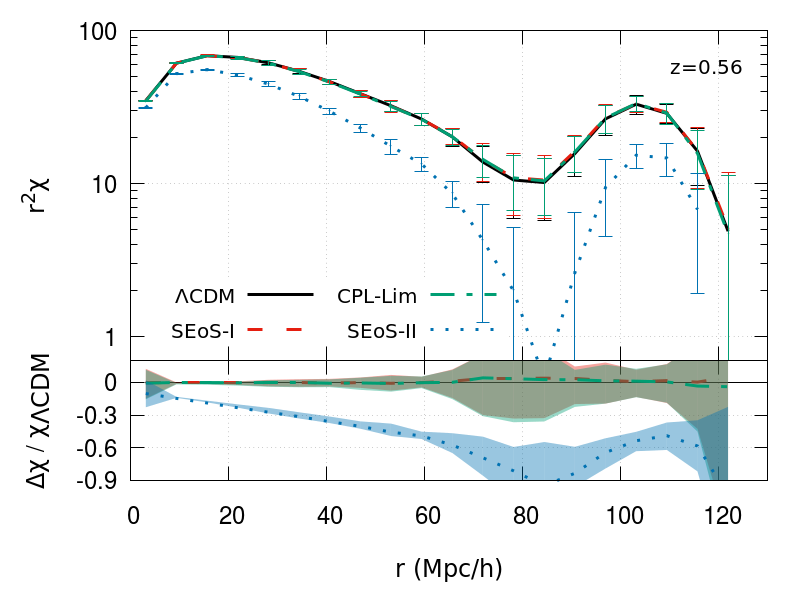
\includegraphics[width=0.5\textwidth,angle=0]{./plots/HS-50_Prom_2PCF_halos_Lb1024_out8}   
		%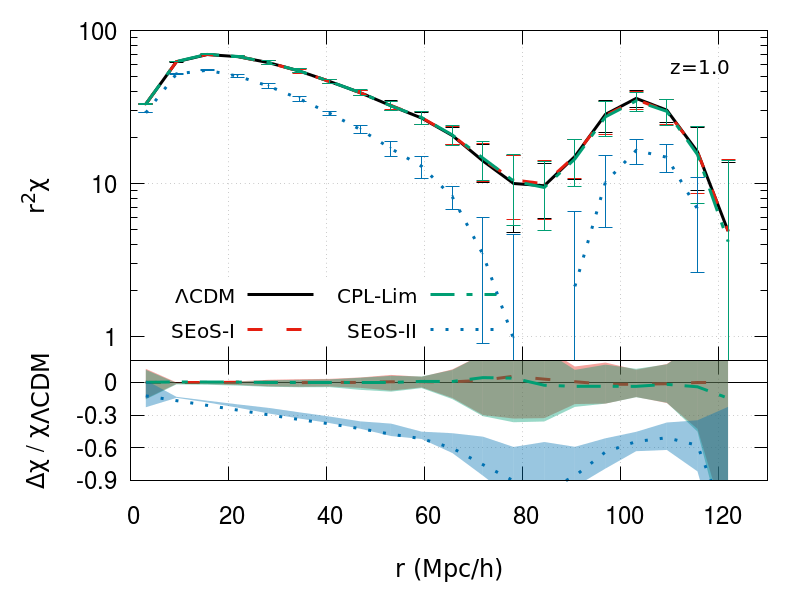
\includegraphics[width=0.33\textwidth,angle=0]{./plots/HS-50_Prom_2PCF_halos_Lb1024_out6} \\
		
	\end{tabular}
	
	\caption{2PCF for all the considered models at redshifts, $z = 0$, $0.28$, and $1.0$ after selecting halos with more than 50 particles. Their respective difference w.r.t. $\Lambda$CDM is shown in {\it middle} and {\it lower} panels. Shaded regions represent  1-$\sigma$ standard deviation, calculated from 5 realizations run with different random seeds. Note: A significant deviation is observed for SEoS-II model from the $\Lambda$CDM at all redshifts.}
	\label{fig:2PCF}
	% \end{center}
\end{figure*}


The two point correlation function (2PCF) remains one of the strongest tools to study the clustering of large scale structure either through galaxies or halos. For this work, we analyze the clustering of DM halos in real space for all the models. Our simulation settings of $L_{\rm box}$= $1024 h^{-1}{\rm Mpc}$ and $Np=1024^3$, allow us to trace up to the Baryon Acoustic Oscillation (BAO) scale.

The measurement of 2PCF between halos is performed with the code called Correlation Utilities and Two-point Estimates (CUTE) \cite{cutecode}\footnote{https://github.com/damonge/CUTE}. The correlation function we measure is estimated by the function:
\begin{equation}
\xi\left(r\right)=\frac{V_{\rm box}\times D_{h}D_{h}\left(r\right)}{V_{\rm bin}\left(r\right)\times N_{h}^{2}}-1,
\end{equation}
where $D_{h}D_{h}$ is the number of halo-halo pairs within a given separation bin of volume $V_{\rm bin}$, $N_{h}$ is the total number of halos in the box, and $V_{\rm box}$ is the volume of the simulation box, i.e., $V_{\rm box}=L_{\rm box}^3$. We set up 20 linearly spaced bins in the range of $r = 0-125~h^{-1} {\rm Mpc}$. For a statistically homogeneous and isotropic field, the halos are only correlated according to their relative distance, $r$. Thus, we present the result of 2PCF as function of $r$ in Figure (\ref{fig:2PCF}) for $z=0,\,0.28,\,1.0$.
%
%
Note that our results are based on the average over 5 realizations of the simulation we run for each model.
Similar to Figure (\ref{fig:pk_nonlinear}), the results are displayed in three panels (\ref{fig:2PCF}). The upper panel focuses on the full 2PCF, the middle one shows the relative difference of models w.r.t. $\Lambda$CDM, and the bottom panel shows a zoom of the relative difference to highlight the deviation of SEoS-I and CPL-lim from $\Lambda$CDM.

%, middle, and lower panels are focusing on the full 2PCF, relative difference of models w.r.t. $\Lambda$CDM, along with the error estimated from 5 realisations for each model, and the zoom in of middle plots to highlight the difference of SEoS-I and CPL-lim from $\Lambda$CDM respectively. 

From the upper panels of (\ref{fig:2PCF}), we observe the BAO feature at a scale of around $r\sim 100 h^{-1} {\rm Mpc}$ in all models, even with the limitation in resolution at those scales. The standard behaviors of the BAO feature are recovered, including the widening of the peak when it goes from high to low redshift.


A significant variation in the 2PCF is observed between SEoS-II and $\Lambda$CDM (see in the middle panels of (\ref{fig:2PCF})). As discussed before, the deviation between SEoS-II and $\Lambda$CDM is mainly governed by the difference in global cosmological parameters, i.e., $\Omega_{m0}=0.334$ and $H_{0} = 73.32$, instead of the $\Lambda$CDM values, $\Omega_{m0}=0.3089$ and $H_{0} = 67.74$. 
%
Thus, we draw the following conclusion. The low clustering signal revealed in the 2PCF of SEoS-II is due to the model with higher DM content leads to a faster growth of structures (see Figures \ref{fig:deltas} and \ref{fig:f_growth}), and ends up with denser but more widely spread halos. In addition, the DE-dominated epoch comes later in this model compared to $\Lambda$CDM, hence the structures tend to virialise earlier. This result also shows the sensibility of halo-clustering on the cosmological parameters. The difference in 2PCF of SEoS-II over $\Lambda$CDM reduces from $\sim 70\%$ at $r = 70 h^{-1} {\rm Mpc}$ to $\sim 20\%$ at $r = 20 h^{-1} {\rm Mpc}$. Note that the errors become relatively high after the scale, $r = 60 h^{-1} {\rm Mpc}$.



%Thus, we draw the following conclusion, the low clustering revealed in the 2PCF of SEoS-II is because the model with the higher DM content leading to a higher $H_{0$} overcoming the structure growth. In addition, DE dominated epoch comes later in this model compare to $\Lambda$CDM, hence the structures tend to virialise earlier. This result also shows us the sensibility of halo clustering on the cosmological parameters. The difference in 2PCF of SEoS-II over $\Lambda$CDM reduces from $\sim 70\%$ at $r = 70 h^{-1} {\rm Mpc}$ to $\sim 20\%$ at $r = 20 h^{-1} {\rm Mpc}$. Note that the errors become relatively high after the scale, $r = 60 h^{-1} {\rm Mpc}$.

 The bottom panel of (\ref{fig:2PCF}) shows that CPL-lim and SEoS-I models remain within  $\sim 1\%$ difference w.r.t. $\Lambda CDM$ up to the scales where the scatter is low, say $r = 60 h^{-1} {\rm Mpc}$. Hence, we conclude that it is challenging to trace the effect of dynamical DE using the halo clustering when we have a $\sim 2\%$ difference in the background expansion rate and the linear growth. We argue that including a larger number of simulations and increasing their accuracy with a larger number of particles and spatial resolution will improve further on this test. 
%---------- flag: UNDER CONSTRUCTION -------- reviewed by Mariana  until this point --------%
\subsection{Halo mass function}
\label{sec:massfunction}

%Another way to understand the growth of structures under different cosmological scenarios is through halos abundance, often referred as Halo mass function (HMF). HFM measures the number of halos per unit volume under certain range of mass bin, $M$ to $M+dM$ at some particular redshift.  We are using the halo mass definition of $M_{200} \equiv \frac{4\pi}{3}200\rho_{c}R^3_{200}$ which corresponds to halos enclosing $200$ times the critical density of our Universe and their corresponding radius $R_{200}$. Recall that halos are found using the \texttt{rockstar} halo-finder. 

%In principle, we know that the impact of dynamical DE is through the expansion history and the growth of structure. Depending on the behavior of EoS, $w(a)$ parameter, the expansion rate, $H(a)$ changes, thus the halos could be more or less clustered and accordingly the abundance changes in the structure formations. Subsequently, the structures can also take longer or lesser time period to form a bound structure under such situations. It is interesting to study their impacts on the halos abundance, often referred as Halo mass function (HMF). HFM measures the number of halos per unit volume under certain range of mass bin, $M$ to $M+dM$ at some particular redshift.  We use the halo mass definition of $M_{200} \equiv \frac{4\pi}{3}200\rho_{c}R^3_{200}$ which corresponds to halos enclosing $200$ times the critical density of our Universe and their corresponding radius $R_{200}$. Recall that halos are found using the \texttt{rockstar} halo-finder. 



\begin{figure*}
	\centering
	\begin{tabular}{cc}
		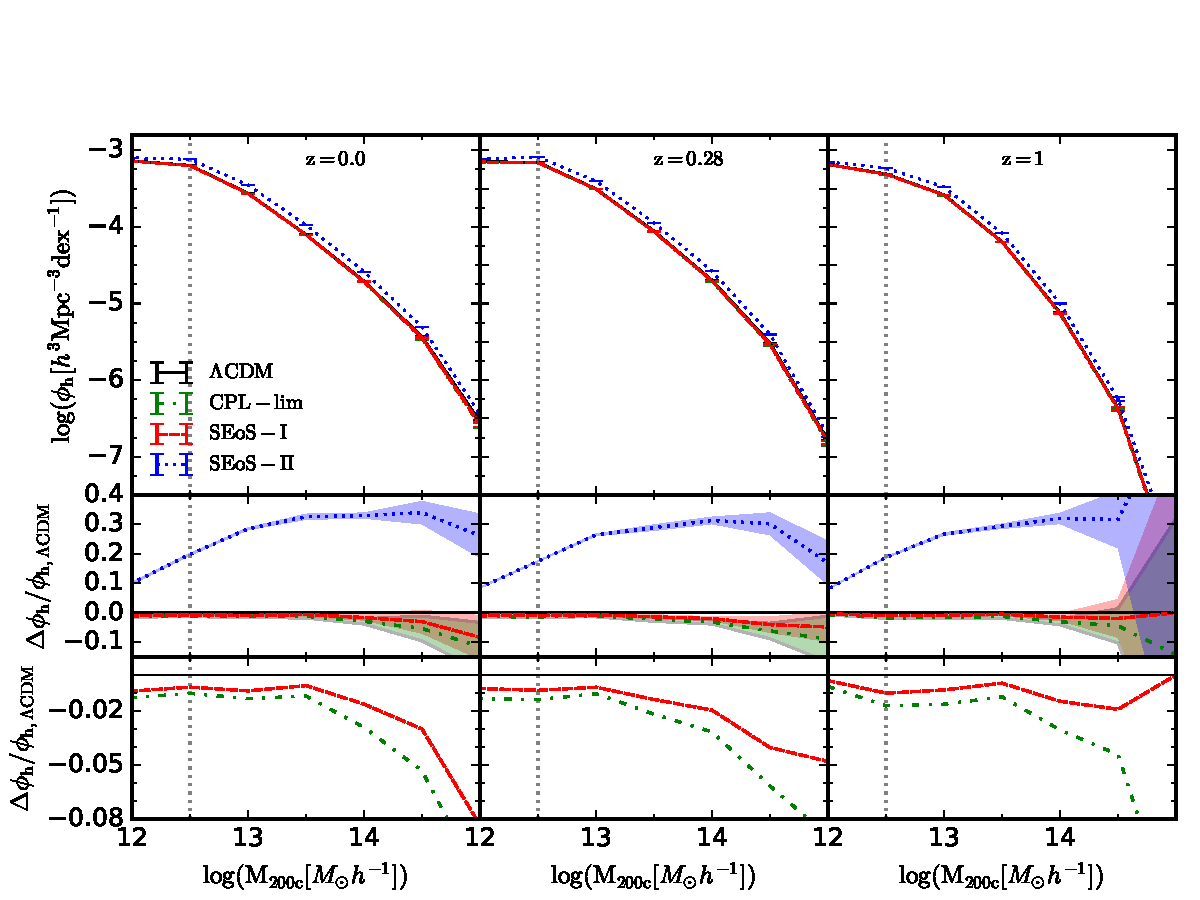
\includegraphics[width=1\textwidth,angle=0]{./plots/halo_mass_function_all_new.pdf} 
		% 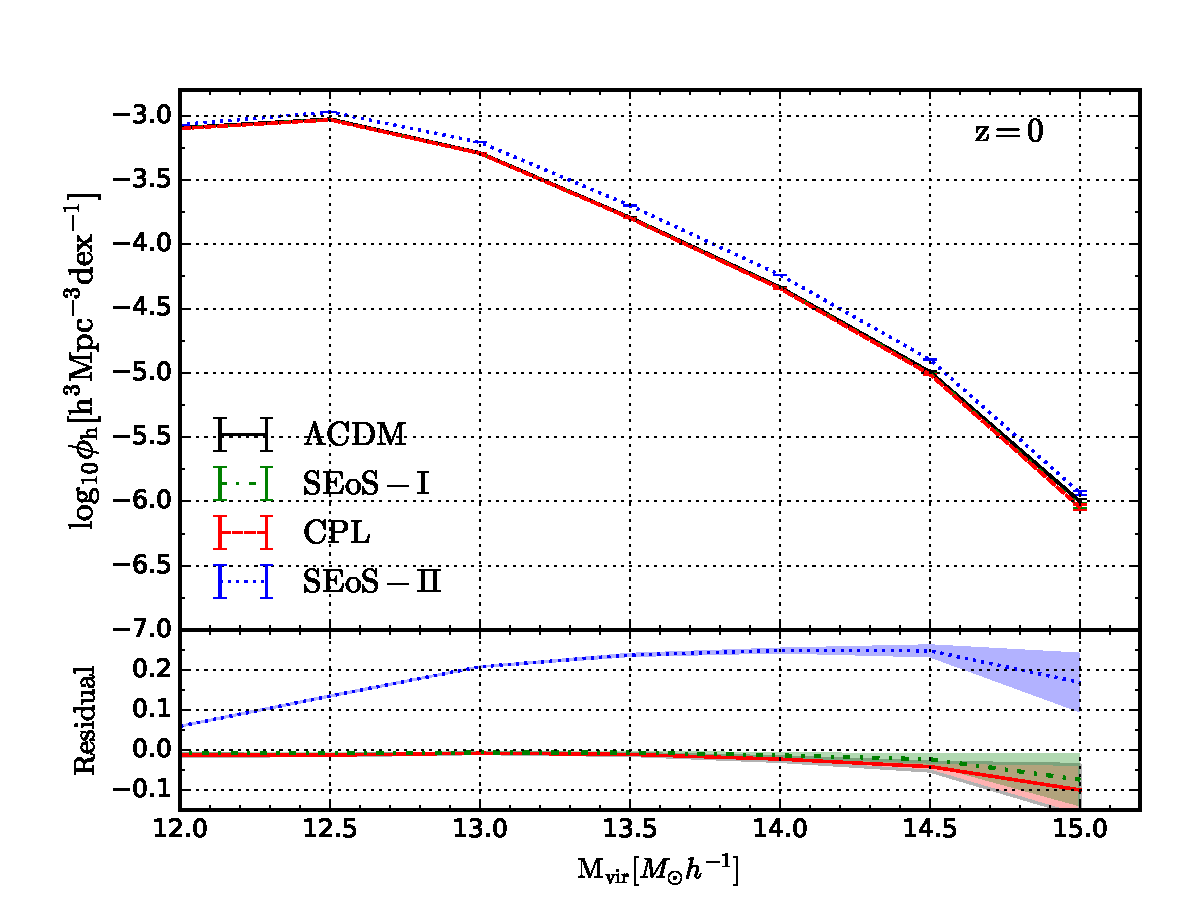
\includegraphics[width=0.33\textwidth,angle=0]{./plots/hmf_diff_11_z0.pdf}   
		% 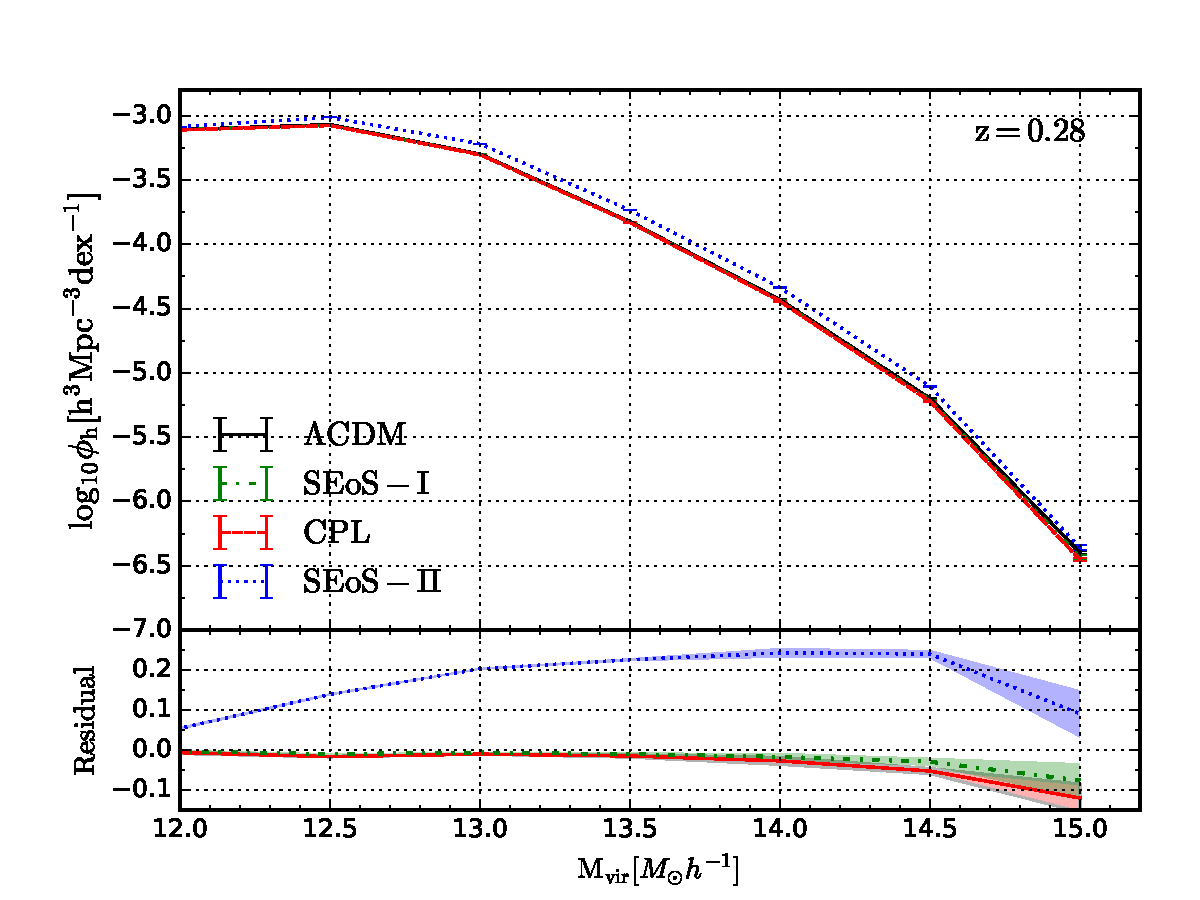
\includegraphics[width=0.33\textwidth,angle=0]{./plots/hmf_diff_9_z0p28.pdf} 
		
		% 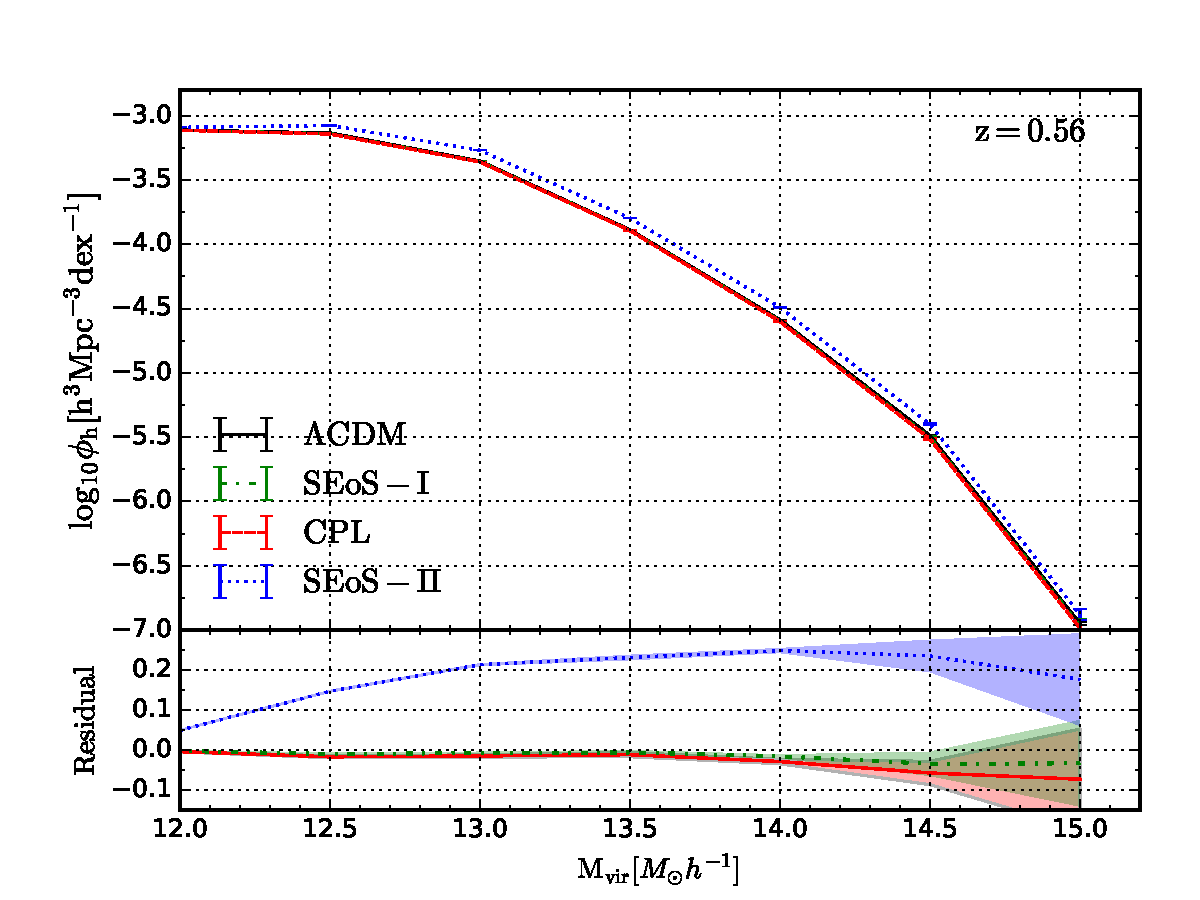
\includegraphics[width=0.5\textwidth,angle=0]{./plots/hmf_diff_8_z0p560.pdf}   
		% 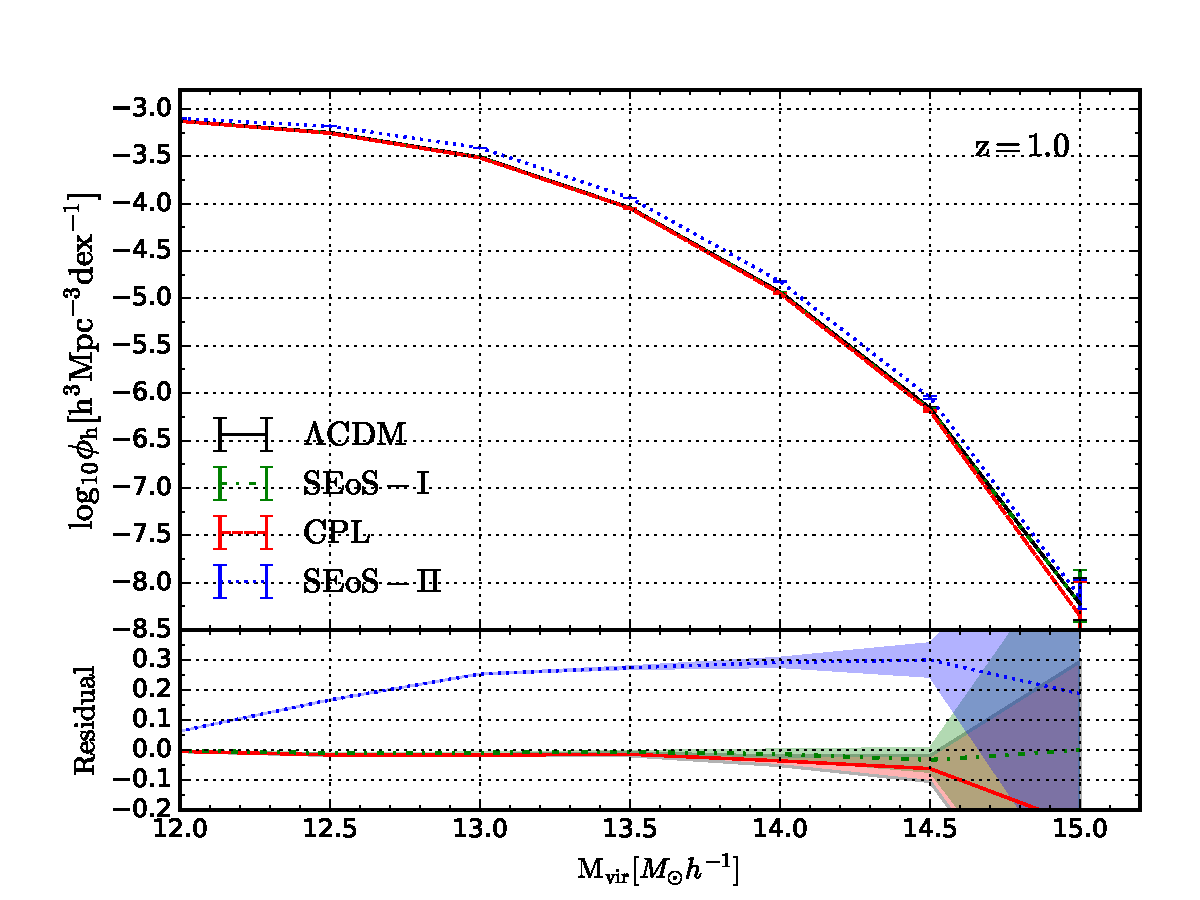
\includegraphics[width=0.33\textwidth,angle=0]{./plots/hmf_diff_6_z1p0.pdf} 
		
	\end{tabular}
	
	\caption{{\it Upper panels:} Differential halo mass functions for all the models at redshifts, $z = 0$, $0.28$, and $1.0$. {\it Middle panels}: The difference w.r.t. $\Lambda$CDM along with their one sigma standard deviation calculated from 5 realizations run under different random seeds (shaded regions). {\it Bottom panels}: Zoom-in plot of the second panel to highlight the differences between the CPL-lim and SEoS-I.
		%Note: A significant variation is observed for SEoS-II model from the $\Lambda$CDM at all redshifts.
	}
	\label{fig:HFM}
	% \end{center}
\end{figure*}


Depending on the behavior of DE, the structure we observed can be more or less clustered, subsequently, it will take less or longer time to form a gravitational bound structure. Such effect is studied via the Halo mass function (HMF). HFM measures the number of halos per unit volume under certain range of mass bin, $M$ to $M+dM$, at some particular redshift.  We use the halo mass definition of $M_{200} \equiv \frac{4\pi}{3}200\rho_{c}R^3_{200}$, which corresponds to halos enclosing $200$ times the critical density of our Universe, and their corresponding radius, $R_{200}$. 
%Note that halos are found using the \texttt{rockstar} halo-finder.

Figure (\ref{fig:HFM}) shows the mean differential HMF of 5 realizations for each model at redshifts $z = 0, 0.28$, and $1$. As expected, SEoS-I has the closest halo abundance to $\Lambda$CDM, followed by CPL-lim and SEoS-II. SEoS-II corresponds to an universe with $\Omega_{m0}=0.334$, so the number density of DM halos is expected to be larger than  for the other models. That is what we find in the HMF throughout the whole mass range and for all the redshift values considered (see the middle panels of Figure (\ref{fig:HFM})). A difference of $\sim 30\%$ in the HMF is observed between SEoS-II and $\Lambda$CDM in the mass range of $10^{13} M_{\odot}h^{-1} < M_{200}< 10^{15} M_{\odot}h^{-1}$. The difference is slightly reduced at both the low and high mass ends. This decrease in HMF at the high mass end is probably because of the difference in DE behavior. However, the most prominent effect is coming from the difference in the global cosmological parameters.% $\Omega_{m0}=0.334$ and $H_{0} = 73.32$.  

The bottom panel of Figure (\ref{fig:HFM}) highlights the main difference in HMF of SEoS-I and CPL-lim from $\Lambda$CDM. Noting that they share the same cosmological parameters: $\Omega_{m0}=0.3089$ and $H_{0} = 67.74$, the main difference is basically driven by the dynamics of DE. We observe that SEoS-I and CPL-lim have lower number of halos compared to $\Lambda$CDM at all mass scales and redshift values.
%  
The lower growth rate of matter overdensities in SEoS-I and CPL-lim w.r.t. $\Lambda$CDM results in a lower number of halos. One can infer from Figure \ref{fig:HFM} that the higher possibility of distinguishing between our  DE models and $\Lambda CDM$ lies in the high-mass halos. Particularly, looking at a mass scale of $M_{200}=10^{14.5} M_{\odot}h^{-1}$, a  significant difference of $\sim 3\%$ to $\sim 5\%$ is observed at $z = 0$ in SEoS-I and CPL-lim, respectively. However, going towards the high-mass limit comes at the cost of bigger uncertainty.
%
The difference in HMF reduces as we go from low to high redshift for both SEoS-I and CPL-lim. 
We argue that increasing the number of particles in the simulation  might help in reducing the uncertainty level and to increase the possibility of distinguish between the models. 
%Again, this is due to the fact that SEoS-I and CPL-lim have slightly higher expansion rates and thus, lower growth rate of matter densities then in $\Lambda$CDM, leading to end up with universe with less number of halos.

%The results of low HMFs observed in both SEoS-I and CPL-lim over $\Lambda$CDM at all mass scales is due to the fact that SEoS-I and CPL-lim have slightly higher expansion rates and thus, lower growth rate of matter densities over $\Lambda$CDM,


\section{Summary and Conclusions}
\label{sec:conclusions}

 In this paper, we presented a set of N-body simulations designed in the framework of dynamical DE models and analyzed their impact on the structure formation. In particular we studied the effect that a rapid dilution in the energy density of DE has on the growth of structure at cosmic scales. To this end, we assumed DE models with an equation of state, $w(z) = w_0 + w_i\frac{(z/z_T)^q}{1+(z/z_T)^q}$, where a  transition, controlled by the value of $q$, occurs between the fixed values $w_0\equiv w(z=0)$ and $w_i\equiv w(z\gg0)$, at an epoch given by $z_T$.

Specifically, we compared a DE model with a steep transition ($q=9.98$) at a late time ($z_T=0.28$)  versus the same model with a smooth transition ($q=1$) at a later time ($z_T=1$). The latter choice of parameters map our EoS to the Chevallier-Polarski-Linder parameterization \cite{Chevallier2001,Linder2003}. We referred to the the first case as the SEoS model, and  we further divided its study in two sets: SEoS-I and SEoS-II, depending on the cosmological parameters $\Omega_{m0}$ and $H_{0}$ used. The SEoS-I model is based on the Planck results (P15)\cite{Ade2016}: $\Omega_{m0}=0.3089$ and $ H_{0}=67.74$, as in $\Lambda$CDM and CPL-lim cases. The SEoS-II model considered $\Omega_{m0}= 0.334$, $H_{0} = 73.22$, the best fit values obtained in \cite{delaMacorra:2015aqf} along with the SEoS parameters. 
 

The structure formation under such DE scenarios was studied through the hacking of the approximated N-body simulation code called L-PICOLA \cite{Howlett:2015hfa}. %\cite{Tassev:2013pn,Tassev:2015mia}.  
The DE models were implemented via their expansion rates, and the DM perturbation solutions into the Lagrangian perturbations method employed in the code.   
%or initial conditions, we modified the 2LPTic code accordingly.
The simulations assume a box of length: $L_{\rm box}=1024 h^{-1}{\rm Mpc}$, and a number of dark matter particles of $N_{p} = 1024^3$ on a mesh, $N_{\rm mesh}= 1024$. In total, we ran 20 simulations, 5 realizations for each model to estimate the cosmic variance errors. Using the output of simulations, we analyzed the non-linear DM power spectrum, $P_{k}$, the number density of the gravitational bound halos, and halo clustering using the two-point correlation function. We discussed our results at redshifts, $z = 0, 0.28, 1$, since $z = 0.28$ and $z = 1$ are the transition redshifts for SEoS models and CPL-lim, respectively. 
%Halo catalogs are generated using the \texttt{rockstar} halo finder \cite{Behroozi2013} and the two point correlation functions were performed using the Correlation Utilities and Two-point Estimates code (CUTE) \cite{cutecode}. 
%The main results and conclusions from our studies are the following:

The main results and conclusions are as follows:
\begin{itemize}
\item %No significant imprint of the steep transition in DE field is found in the structure formation but we observed the impact of DE in the non-linear regimes. %
The calculated non-linear power spectra, $P_{k}$, of SEoS-I and CPL-lim models presented deficits in power w.r.t. $\Lambda$CDM throughout all $k$-modes. Such behaviour is expected due to the dynamics of DE, i.e., less negative values of the DE EoS and relatively larger expansion rate than in $\Lambda$CDM trigger a slowdown in the growth of structure. This result is consistent with the linear matter perturbations studies. The differences remain within $\sim 2\%$ and $\sim 3\%$ throughout all $k$ scales at $z = 0$ for SEoS-I and CPL-lim, with a slight increase at non-linear regimes. 
The reduction in the deviation from $\Lambda$CDM for higher redshift values is also showing the effect of the dynamics of DE. However, no significant imprint of the steep transition in the DE component is observed in the structure formation.
%As expected, SEOS-I is the closest one to $\Lambda$CDM, followed by CPL-lim and SEoS-II.

The $P_{k}$ of SEoS-II showed up relatively different behaviors. Specifically, a deficit in power at the linear scales and a closer  value to $\Lambda$CDM as it goes from linear to non-linear regimes. Such behavior in SEoS-II is expected for an universe containing more DM  $\Omega_{m0} = 0.334$ and with $H_{0} = 72.23$, instead of the standard values $\Omega_{m0} = 0.3089$, and $H_{0} = 67.74$. Thus, we conclude that the behavior of DE in SEoS-II model is sub-dominant compared to the effect of  changing $\Omega_{m0}$ and $H_{0}$.

\item We discussed how the differential halo mass functions (HMF) were effected by the behavior of DE models. The results of lower HMF observed in SEoS-I and CPL-lim as compared to $\Lambda$CDM at all mass-scales, occurred  as expected. The lower growth rate of matter densities in SEoS-I and CPL-lim w.r.t. $\Lambda$CDM results in a smaller number of bounded halos. The deviation w.r.t.$\Lambda$CDM of SEoS-I and CPL-lim reduces with the increase of redshift. The chances of distinguish between these models from $\Lambda$CDM increases at the high mass end. %Again, we observed reduced in deviation of SEoS-I and CPL-lim with the increase of redshifts.
The SEoS-II model has a value of $\Omega_{m0} = 0.334$, which in turns has a higher HMF, as predicted. The difference reaches up to $\sim 30\%$ deviation from $\Lambda$CDM at $ 10^{14.5}M_{\odot}h^{-1}$, at the considered redshifts.
%As such no variation is observed with redshift in case of SEoS-II.}
%are evolved with slightly higher expansion rates and thus,#
%Again, we observed reduced in deviation of SEoS-I and CPL-lim with the increase of redshifts.

\item We quantified the 2PCFs of SEoS-I and CPL-lim models and both remained within $\sim 1-2\%$ difference w.r.t. $\Lambda$CDM up-to $r = 60 {\rm Mpc} h^{-1}$. At larger scales, the accuracy of numerical experiments makes it challenging to state robust conclusions, but they behave in a consistent way. On the other hand, SEoS-II which was the best-fit model in  \cite{Jaber:2017bpx}, shows a significant difference throughout all $r$ scales. Such deviation reduces as we go from large to small scales in $r$. The deviation reaches up to $\sim 60\%$ at $r = 60 h^{-1} {\rm Mpc}$. We conclude that including the non-linear growth is critical in order to asses the viability of DE models.


\item Although not surprisingly for approximated simulations \cite{2016JCAP05051S}, the results of halo 2PCF and HMF might be biased by the ability of experiments to resolve halo mass and size, while $P_{k}$, in turn, uses the particle distribution. However the general trend of results is consistent across all tests.

\item We point out that having a tool to study LSS based on N-body simulations that run at low computational cost, and which simultaneously recovers the LSS accurately under the dynamical DE scenarios through L-PICOLA\cite{Howlett:2015hfa}, would  be deeply useful to understand the nature of DE. Particularly, it would prove very useful to provide constraints on DE models after running multiple sets of simulations on a wider range of cosmological and DE EoS parameters.

%Overall low clustering effects were depicted for SEoS-II at the redshift we considered but there is a significant deviation from $\Lambda$CDM through out all $r$ scales. Following the trend of higher clustering at low $r$ mode, then even lowering the clustering effect with the increase of $r$.} changes 

\end{itemize}

In conclusion, we state that our results from the non-linear structure formation are consistent with the behaviour of DE, their background and linear perturbation theories. Differences found in SEoS-I and CPL-lim models are directly driven by the DE dynamics. The deviation observed in SEoS-II is entangled with the effect of cosmological parameters and DE behavior. 

We recall that SEoS-II is the best-fitted model of SEoS found in \cite{Jaber:2017bpx}. 
\cite{Jaber:2017bpx} used the observational points from the six-degree-field galaxy survey (6dFGS \cite{Beutler:2011hx}), Sloan Digital Sky Survey Data Release 7 (SDSS DR7 \cite{Ross:2014qpa}) and the reconstructed value (SDSS(R)  \cite{Padmanabhan2pc}), as well as the complete BOSS sample SDSS DR12 (\cite{Alam:2016hwk}), and the Lymann-$\alpha$ Forest (Ly$\alpha$-F) measurements from the Baryon Oscillation Spectroscopic Data Release 11 (BOSS DR11 \cite{Font-Ribera:2013wce}, \cite{Delubac:2014aqe}), along with the local Hubble constant measurement by (\cite{Riess:2016jrr}) and the compressed CMB likelihood from Planck collaboration (\cite{Ade2016, mukherjee, planck15DE}) to constraint the model. That being said, the large deviations w.r.t. $\Lambda$CDM in the non-linear structure formation found for SEoS-II, points out to the necessity  of extending the study of DE models beyond the linear regime.
%This implied that significant different observed in SEoS best fits values, could be improved further in future.
%The best fit values of model parameters and ($\Omega_{m0}=0.334$, $ H_{0}=72.23$) we used for SEoS-II obtained \cite{Jaber:2017bpx



Note that our work was mainly focused on some particular DE parametrization, but the code can be easily extended to other dynamical DE models as long as the DE field remains homogeneous. Even though there is still room to further test SEoS models by increasing the number and accuracy of simulations, we are in progress of including other dynamical DE models such as the tachyon DE field and interacting DM-DE models in up-coming projects.  A strategy like the one presented in this paper is particularly appealing under the light of upcoming high accuracy galaxy surveys like DESI \cite{Aghamousa:2016zmz}.

\appendix
\section{The linear power spectrum}
\label{app:Pk_initial}
The initial linear power spectra, $P_{k,lin}$, at redshift $z_{in}=49$ from \texttt{CAMB}, used in the simulations are shown in Figure (\ref{fig:pk_initial}). 
The black solid and blue dotted lines correspond to the power spectra obtained with P15 ($\Omega_{m0} = 0.308$ and $H_{0} =0.6774$), and SEoS-II case: ($\Omega_{m0} = 0.334$ and $H_{0} =73.22$), respectively. 
The value for other parameters can be found in Table \ref{table:COLA_models}.  
To compare, we also include the  power spectrum at $z = 0$, $P_{k,lin}$  computed from \texttt{CAMB} in black dash-dotted and red dashed lines for $\Lambda$CDM and SEoS-II cases, respectively. 
We found that, even at the initial power spectrum at $z_{in}=49$, there is an enhancement in power at the high $k$-modes compared to intermediate scales, followed by a deficit in power for the low $k$-modes. A similar behavior is observed at $z = 0$ with a slight increase at high $k$-scales. These discrepancies are expected and they arise mainly due to the difference in the amount of dark matter contained in the simulations. 
%Such behaviors are well studied in literature with the $\Lambda$CDM model on varying the $\Omega_{m0}$, $w_{0}$ and $H_{0}$ values. We do observe a similar behavior in the non-linear power spectrum calculated on the output of our simulations, i.e., on comparing the SEoS-II to that of $\Lambda$CDM.

%\begin{figure}
%\centering 
%\hfill
%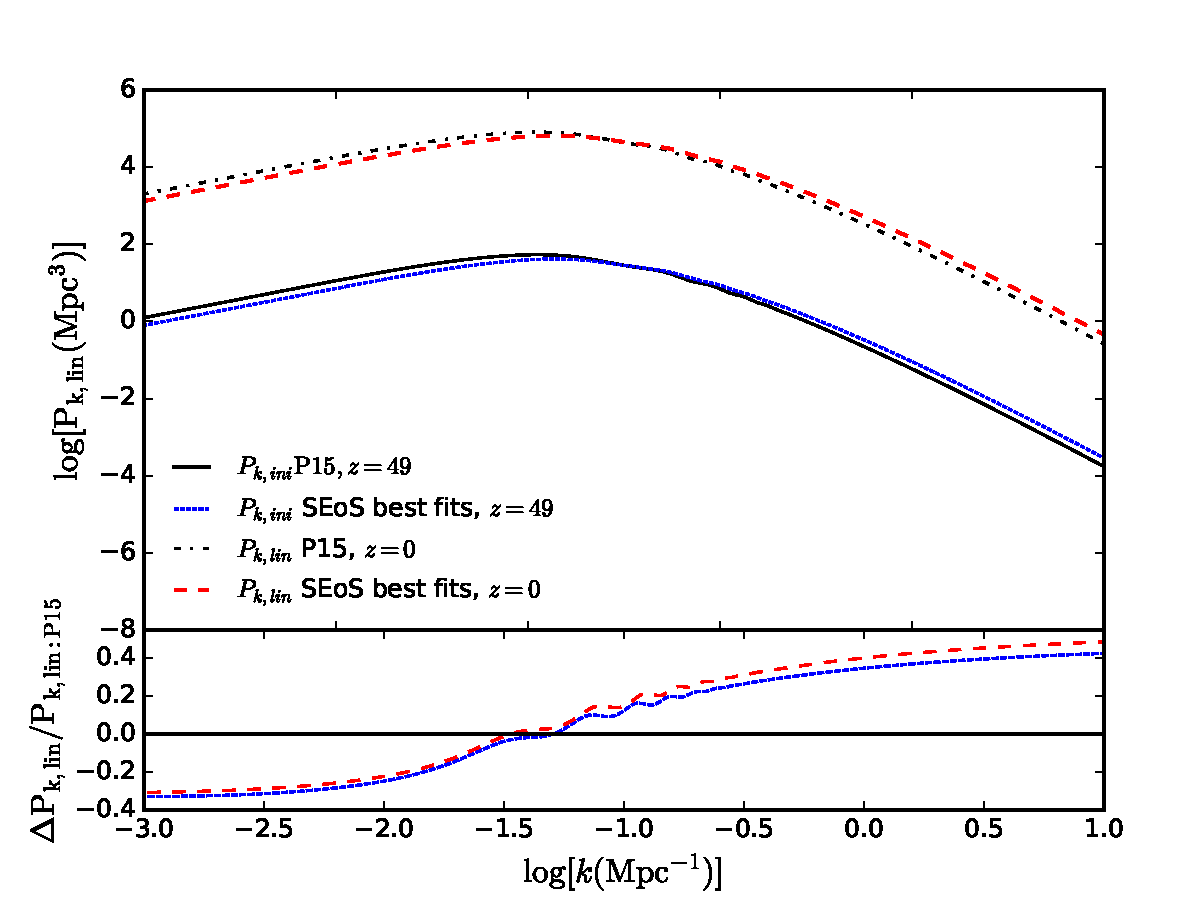
\includegraphics[width=0.6\textwidth,angle=0]{./plots/pk_camb_new.pdf}
%\caption{The initial linear power spectrum from \texttt{CAMB} at redshift $z_{in}=49$, used for our simulations. The black solid and blue dotted lines correspond to the power spectra with P15 cosmological values $\Omega_{m0} = 0.308$ and SEoS-II best fit values, $\Omega_{m0} = 0.334$ respectively. Their corresponding CAMB output at $z=0$ are also included for comparison in red dashed and black dash-dotted lines respectively. 
%\label{fig:pk_initial}}
%\end{figure}

\begin{figure}
\centering 
%\hfill
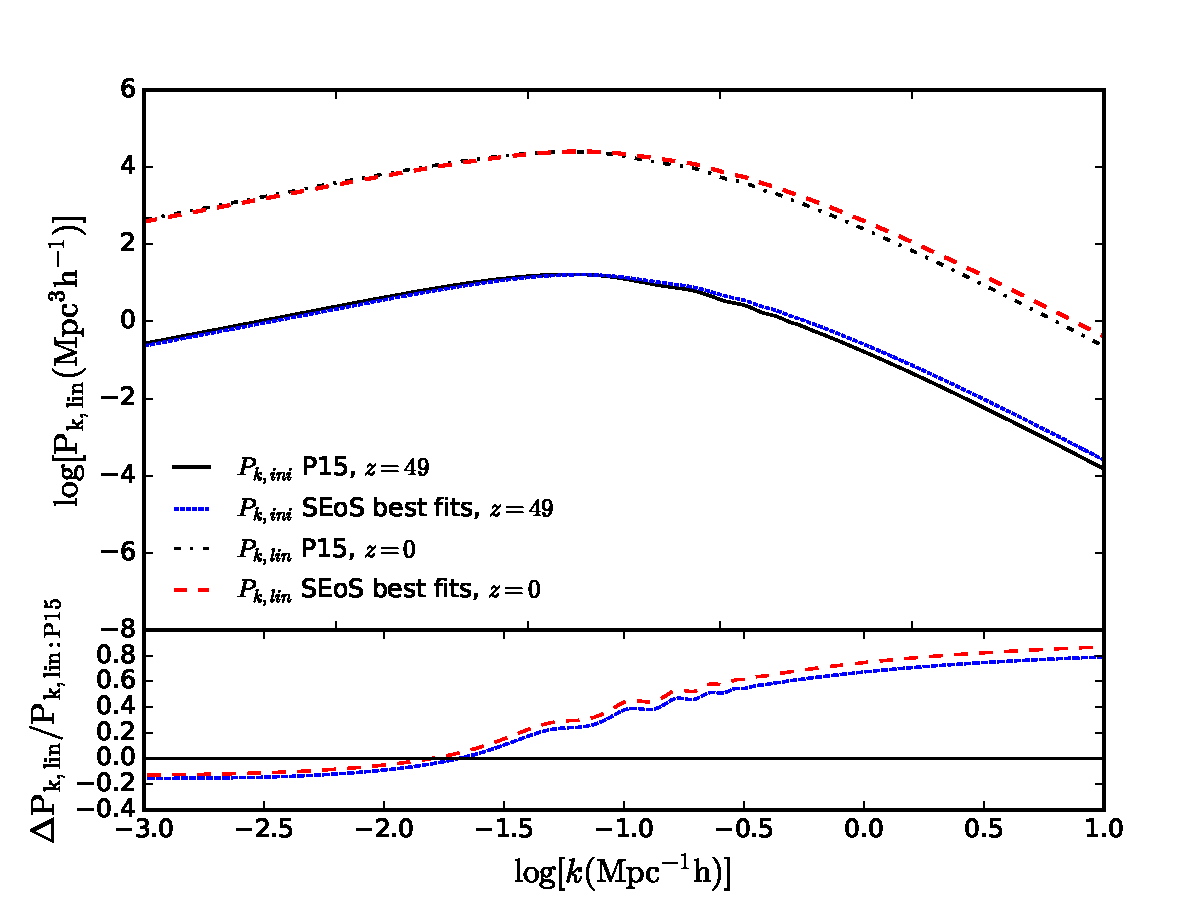
\includegraphics[width=0.6\textwidth,angle=0]{./plots/pk_camb_new2.pdf}
\caption{The initial linear power spectrum from \texttt{CAMB} at redshift $z_{in}=49$, used for our simulations. The black solid and blue dotted lines correspond to the power spectra with P15 cosmological values $\Omega_{m0} = 0.308$ and SEoS-II best fit values, $\Omega_{m0} = 0.334$ respectively. Their corresponding \texttt{CAMB} output at $z=0$ are also included for comparison in red dashed, and black dash-dotted lines, respectively. 
\label{fig:pk_initial}}
\end{figure}

\section*{Acknowledgements}
NCDevi thanks Hans Winther and Marc Manera for the fruitful discussions and feedback. 
NCDevi acknowledges support from a DGAPA-UNAM post-doctoral fellowship and CONACyT Fronteras de la Ciencia grant 281. %NCDevi thanks the support provide by LACEGAL during which this project is completed. 
NCDevi acknowledges support from the European Commission's Framework Programme 7, through the Marie Curie International Research Staff Exchange Scheme LACEGAL (PIRSES-GA-2010-269264) when main research of the work are obtained.
%
M. Jaber acknowledges the support of CONACYT graduate fellowship and that of the Polish Ministry of Science and Higher Education MNiSW grant DIR/WK/2018/12.  %LSST
%
Part of this work was supported by the ``A next-generation worldwide quantum sensor network with optical atomic clocks'' project, which is carried out within the TEAM IV programme of the Foundation for
 Polish Science co-financed by the European Union under the European Regional Development Fund.
 %TEAM
OV and G Aguilar acknowledge support from UNAM PAPIIT grant IN112518. G. Aguilar thanks support from a CONACyT graduate fellowship.
%We acknowledge support from Project IN103518 PAPIIT-UNAM and PASPA-DGAPA, UNAM.
M. Jaber and Axel de la Macorra acknowledge support from Project IN103518 PAPIIT-UNAM and A. De la Macorra of PASPA-DGAPA, UNAM. HV acknowledges support from IN101918 PAPIIT-UNAM Grant. The authors acknowledge DGTIC-UNAM for facilities on the Supercomputer MIZTLI at DGTIC-UNAM and also the ATOCATL Cluster Supercomputer of IA-UNAM.
The authors also thank Julio César Clemente for his help in setting up software in those supercomputer.  



\bibliographystyle{jhep}
\bibliography{refs}
\end{document}


\begin{figure*}
     \centering
     \begin{tabular}{cc}
        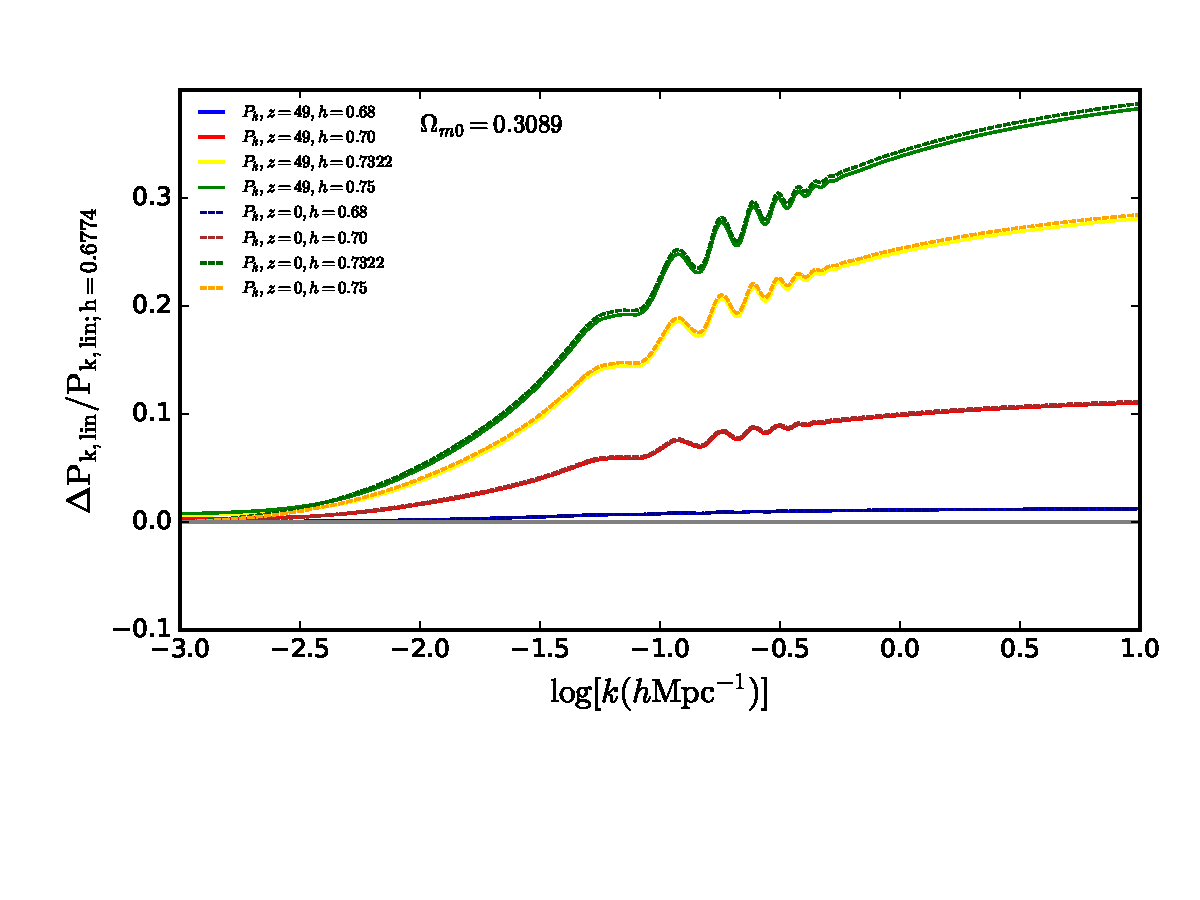
\includegraphics[width=\textwidth,angle=0]{./plots/pk_initial_varying_withh.pdf}   
%        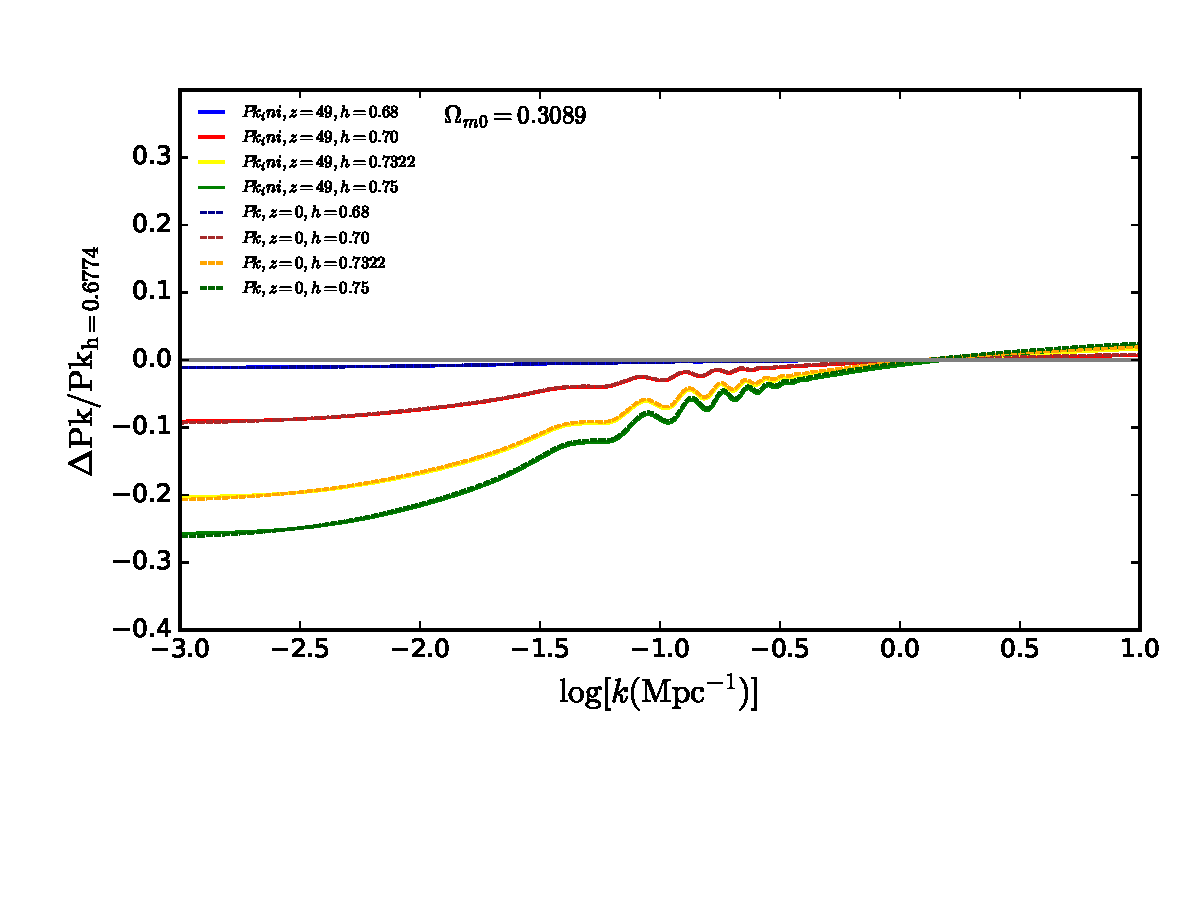
\includegraphics[width=0.5\textwidth,angle=0]{./plots/pk_initial_varying_h.pdf} \\

     \end{tabular}

\caption{{\it Left panel:} 
The linear power spectra for different values of $h$ for $\Lambda$CDM model from \texttt{CAMB} setting $\Omega_{m0}=0.3089$. The relative differences are calculated w.r.t. $h=0.6774$. {\it Right panel:} With the correction of each $h$ value.
}
\label{fig:pk_liner_h}
% \end{center}
\end{figure*}

\begin{figure}
\centering 
%\hfill
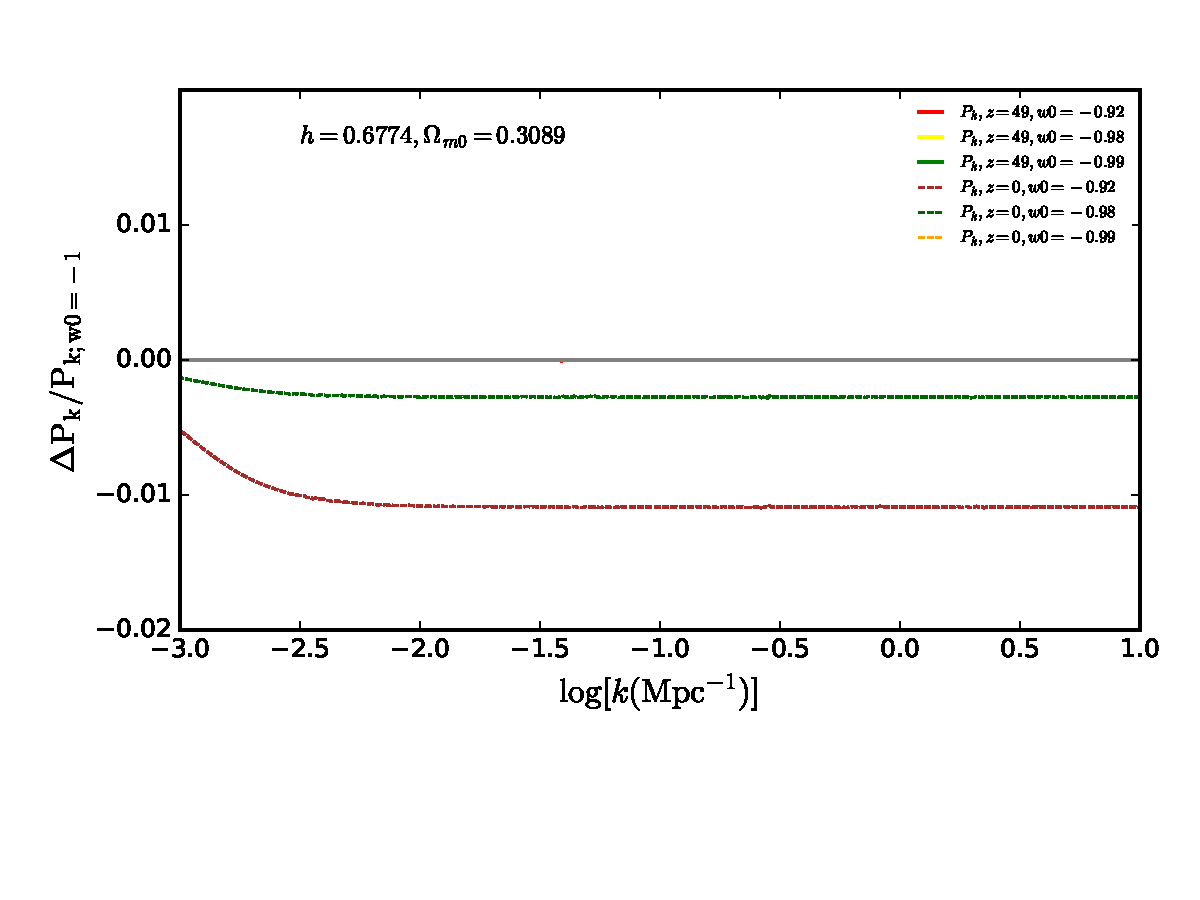
\includegraphics[width=\textwidth,angle=0]{./plots/pk_initial_varying_w0.pdf}
\caption{The linear power spectrum for a CPL like model, where $w0$ acts like $\Lambda$CDM equation of state $w$ at $z_{in}=49$ and $z=0$ from \texttt{CAMB}. With $w0=-0.99$(orange dotted),$-0.98$(green dotted),$-0.92$(red dotted) at $z=0$. The ratio is calculated with the power spectrum of $w0 =-1$. All of them are showing the same power spectrum at $z=49$. However, the up most different we took in the equation of state ($w0=-0.92$) and ($w0 = -1$) with different of $3\%$ shows a difference of $1\%$ on in the $P_{k,lin}$ 
\label{fig:pk_linear_w}}
\end{figure}



\begin{figure}
\centering 
%\hfill
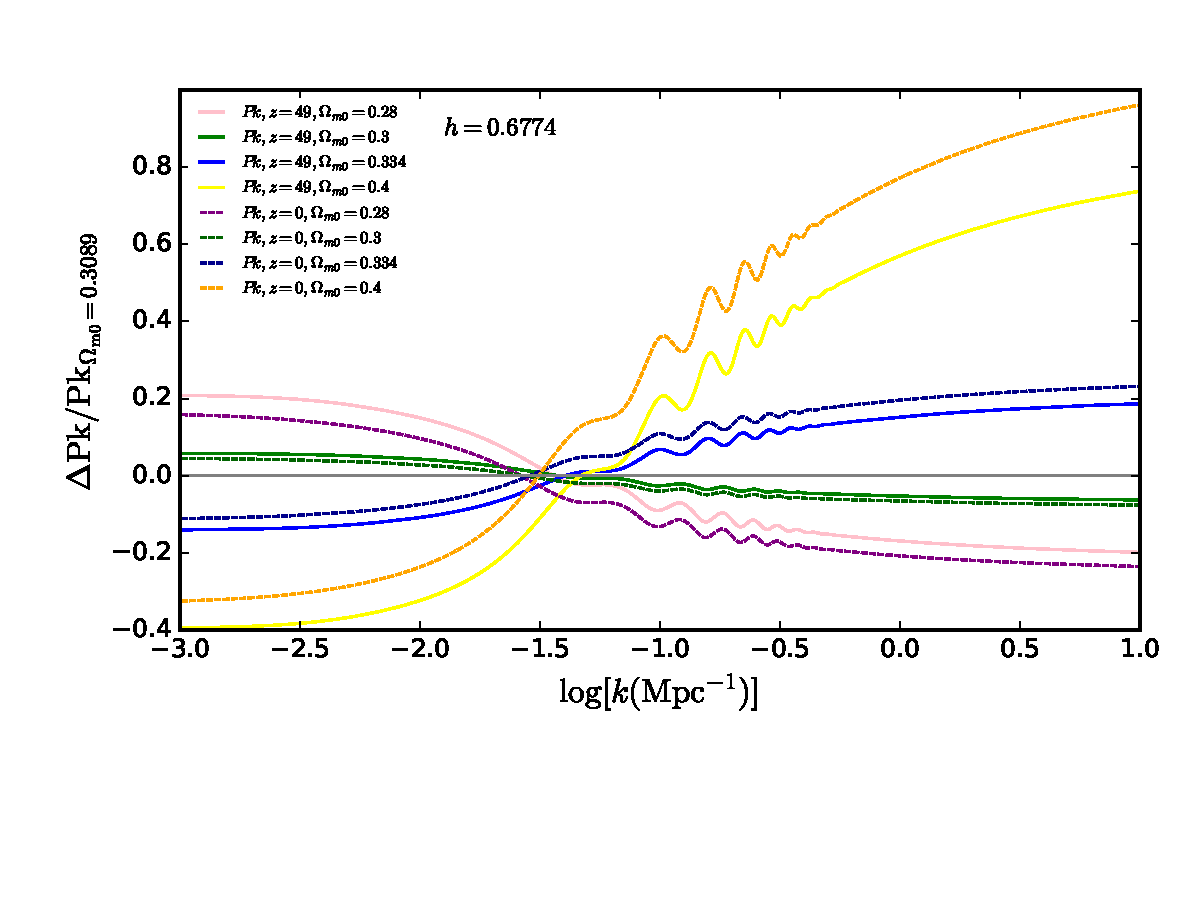
\includegraphics[width=0.6\textwidth,angle=0]{./plots/pk_initial_z0n49_varying_om_new.pdf}
\caption{The linear power spectra, $P_{k,lim}$ for the $\Lambda$CDM model at $z=0$ and $z = 49 $ from \texttt{CAMB}, on varying $\Omega_{m0}$ values. The blue lines correspond to the power spectra obtained for $\Omega_{m0} = 0.334$. The ratio is calculated w.r.t. $P_{k,lim}$ of $\Omega_{m0} =0.3089$.
\label{fig:pk_linear_om}}
\end{figure}


The $P_{k}$ of SEoS-II shows relatively different behavior with a deficit in power at the linear scales and the difference reduces when it goes from linear to non-linear regimes. A maximum deviation of $\sim 30\%$ at low scales (say at $k = 0.01{\rm Mpc}h^{-1}$) is observed in $P_{k}$ of SEoS-II. Such behavior is expected due to the different in the dark matter contained and $H_{0}$ for SEoS-II over $\Lambda$CDM. As such no significant impact of steep transition in DE field is found on the structure formation.
N-body simulations under the Abacus project where 40 sets are based on the constant equation of state DE ($wCDM$) model. % are released in \cite{Garrison:2017ssz} where 40 sets are based on the constant equation of state DE ($wCDM$) model with Planck 2015 cosmology.
 %in 1.1 $h^{-1}$ Gpc and $720 h^{-1}$ Mpc boxes. 
 %The halo catalogues and particles subsamples ranging from z = 1.5 to 0.1 are publicly available \footnote{https://lgarrison.github.io/AbacusCosmos.}.
\cite{Lawrence+2017} provided the results of the Chevallier-Polarski-Linder (CPL) parameterization \cite{Chevallier2001,Linder2003} for DE, including also massive neutrinos. The latter was run with the Hardware-Hybrid Cosmology Code (HACC), a high-performance cosmology code (see \cite{Heitmann:2015xma} for more details).

In addition to the high-resolution N-body simulations, several fast-approximated N-body simulations have been developed to mock the galaxy catalogs accurately on vast scales. % and at fast rate.
However, their primary goal is to estimate the covariance matrix accurately for large scale structure surveys, and so they use the standard $\Lambda$CDM model. 
%
The list includes PTHalos \cite{Scoccimarro:2001cj}, Quick Particle Mesh Simulations(QPM) \cite{White:2013psd}, Effective Zel'dovich approximation mocks(EZmocks) \cite{Chuang:2014vfa}, PINOCCHIO \cite{Monaco:2001jg, Monaco:2013qta}, PATCHY \cite{2014MNRAS.439L..21K}, COmoving Lagrangian Acceleration (COLA) \cite{Tassev:2013pn,Tassev:2015mia}, an upgraded light cone enabling parallel version of COLA: L-PICOLA \cite{Howlett:2015hfa}, etc.  Each of them has its own approximation methods and applications on mocking the catalogs and analyzing uncertainties on several on-going surveys. 

 
For our purpose, we employ the L-PICOLA code\cite{Howlett:2015hfa} after incorporating the dynamical DE through the expansion history, first and second-order Lagrangian Perturbation Theory (2LPT) approximation. The COLA method used in \cite{Howlett:2015hfa} was introduced with an idea to capture the large scale structure (LSS) accurately within few time steps, with the less use of computational resources but still enabled to small scales  accurately  \cite{Tassev:2013pn,Tassev:2015mia}. It is done successfully by implementing the solutions of the first and second-order dark matter perturbations that guarantee to capture the LSS to some extent. Along with this idea of COLA and the large number of cosmological models we have, the implementation of such models in fast COLA-like N-body simulations would be an efficient and adequate way to understand their effects in the regimes required for the upcoming galaxy surveys.
 
An attempt in this regard has already made for the modified gravity(MG) theories in the referred code called MG-COLA \cite{Winther:2017jof}.
Their studies pointed out that, in general, the COLA approach overestimates the halo mass function even for the $\Lambda$CDM model but preserving the difference of MG w.r.t. $\Lambda$CDM accurately. For our case, we are choosing the dynamical DE models of CPL-like parameterization  \cite{Chevallier2001,Linder2003} and the steep equation of state parameterization \cite{Jaber:2017bpx}. We perform a comparative study w.r.t. $\Lambda$CDM. The main idea of this work is not only to understand the effect of these DE models but also to confront our understanding in disentangling their effect from the global cosmological parameters such as $\Omega_{m0}$ and $H_{0}$, through LSS.

The paper is structured as follows: In Section \ref{sec:method}, we describe the models, their background evolution, and the dark matter perturbations up to second-order (see \cite{Bernardeau:2001qr} for a review). In Section \ref{sec:nonlinear}, we discuss the COLA method employed by the N-body simulation called L-PICOLA \cite{Howlett:2015hfa}. The results in terms of the dark matter power spectrum, the halo mass function, and the two-point correlation function of halos are discussed in section  \ref{sec:results}. We summarise and conclude in Section \ref{sec:conclusions}.

The fiduciary cosmological parameters used for this work are $\Omega_{m0} = 0.3089$, $\Omega_{b0} = 0.045$, $h = 0.6774$, $\sigma_{8} = 0.8159$,and $n_s = 0.9667$.

\section{Cosmological models}
\label{sec:method}
This section focuses on the DE models we considered for our analysis. We discuss their background expansion history and the evolution of their matter perturbations up to second-order. Such perturbative solutions are used in generating the initial conditions for the N-body simulations. 

\subsection{Dark energy model and background expansion}
\label{sec:background}

\begin{figure}
\centering 
%\hfill
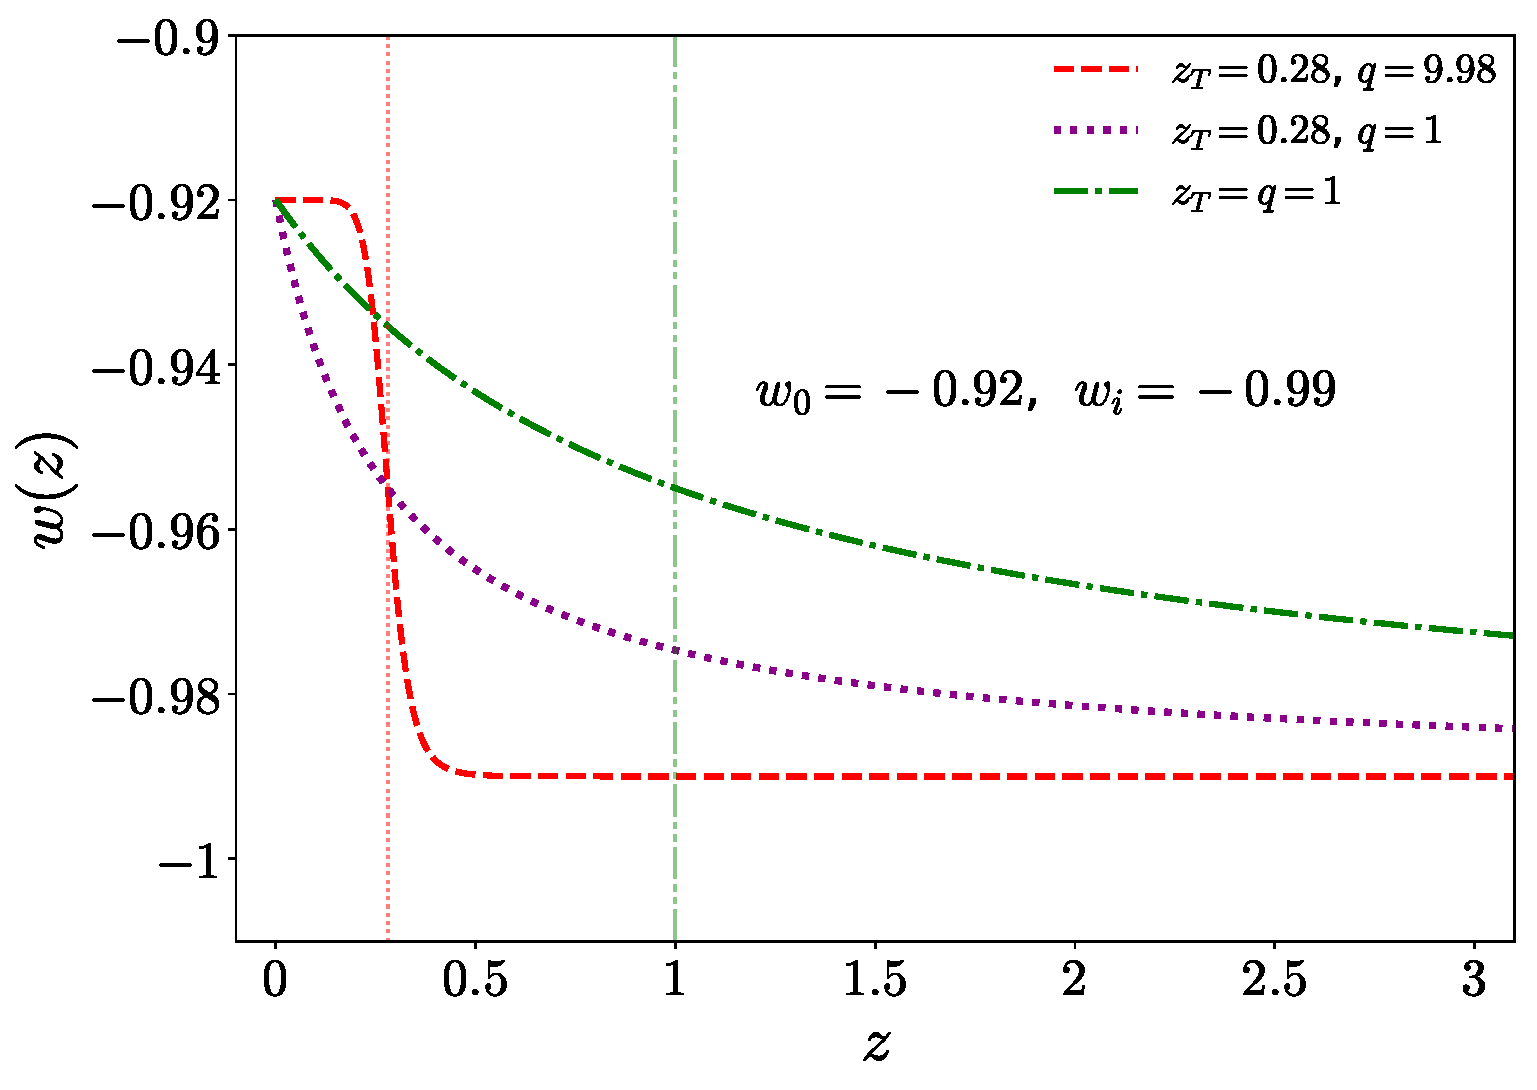
\includegraphics[width=0.6\textwidth, angle=0]{./plots/fig1_2a.pdf}
\caption{\label{fig:eosqs} Evolution of the proposed equation of state for DE  \eqref{eq:seos} with fixed parameters $w_0=-0.92$, $w_i=-0.99$. The red dashed line corresponds to $z_T=0.28$ and $q=9.98$ which we refer to as SEoS-I hereafter. The green dot-dashed line with $q=z_T=1$ represents the CPL limit of SEoS model with the CPL parameters: $w_0 =-0.92$ and $w_a =-0.07$. The magenta dotted line with $z_T=0.28$ and $q=1$ represents an intermediate case between them. The transition between two pivotal points is marked with the vertical lines for SEoS-I and CPL limit that are occurring at $z_T=0.28$  and $z_T=1$, respectively. The value $z_T$ is defined as $z$ where $w(z_T) = (w_0+w_i)/2$.% Focusing at redshift $z=0.28$, the difference of $\sim 4\%$ is observed between SEoS-I and $\Lambda$CDM whereas CPL has $\sim 7\%$. Similarly at $z=1$, the difference for SEoS and CPL limit reduces to $\sim 1\%$ and $\sim 5\%$ respectively. After $z=0.5$, the SEoS remains to be within $1\%$ throughout redshifts while CPL limit becomes $3\%$ only after $z=2$. For redshifts $z\geq10$, all models displayed are of the order $1\%$ difference from $\Lambda$CDM.
}
\end{figure}

In a phenomenological approach, dark energy models are parametrized through its equation of state (EoS), $w(z) \equiv \frac{{\rm p_{DE}}(z)}{{\rm \rho_{DE}}(z)}$, which describes the evolution of DE pressure to its density as a function of time within a set of free parameters. 
Several forms of $w(z)$ have been proposed in the literature, (see for instance, \cite{Chevallier:2000qy, Linder2003, Doran:2006kp, KraussJonesHuterer2007, Linder:2006ud, Rubin:2008wq, 2009ApJ:703:1374S, 2010PhRvD..81f3007M, Hannestad:2004cb, Jassal:2004ej, Ma:2011nc, Huterer:2000mj, Weller:2001gf, Huang:2010zra, Barboza:2008rh}). 
 Among them, the so-called Chevallier-Polarski-Linder (CPL) parameterization \cite{Chevallier2001,Linder2003} is one of the most widely studied parameterization to the DE equation of state and is given by:
\begin{equation}
w(z) =w_{0}+w_{a}\frac{z}{1+z},
\label{eq:wcpl}
\end{equation}
where $w_{0}$ and $w_{a}$ are constant parameters representing the present value of the EoS and its overall time evolution, respectively. Current observational constrains on CPL parameters are presented in \cite{Linden:2008mf}. 

Within the framework of General Relativity, for a late-time, flat, homogeneous and isotropic universe (i.e.,  governed by the FLRW metric), filled with non-relativistic dark matter (DM) and the DE component, i.e.,  $\Omega_{DE} + \Omega_{m} = 1$, the Hubble expansion rate is governed by
\begin{equation}
\frac{H(z)^2}{H_{0}^2} = \Omega_{m0} (1+z)^{3} + (1- \Omega_{m0}) F(z),
\label{eq:hubble}
\end{equation}
where $H_{0}$ and $\Omega_{m0}$ represent the present day values of Hubble rate and matter density, respectively. The DE density, $\Omega_{DE}(z) = (1-\Omega_{m0})F(z)$ evolves with redshift, $z$ as 
\begin{equation}
F(z) = \exp\left[3 \int_{0}^{z} (1+w(z^{\prime}))/(1+z^{\prime})dz^{\prime}\right].
\label{eq:CPL}
\end{equation}
%\textcolor{gray}{}
In this work, we consider a more general EoS of DE other than \eqref{eq:wcpl}, inspired by  quintessence fields dynamics \cite{delaMacorra:2015aqf}, a parametrization described by:
%
\begin{equation}
\label{eq:seos}
w(z) = w_0 + (w_i-w_0)\frac{\left(z/z_T \right)^q}{1+\left(z/z_T \right)^q}.
\end{equation}
%
where $w_i$ and $w_0$ represent the value of $w(z)$ at high redshifts and at present day, respectively. Here the function, $f(z) = \frac{\left(z/z_T \right)^q}{1+\left(z/z_T \right)^q}$ with a transition redshift, $z_{T}$, and a steepness parameter, $q$, governs the dynamics of the parametrization between two pivotal values ($w_i$,$w_0$). For instance, in case of $f(z) =0$ at $z=0$, EoS becomes $w(z) = w_{0}$; at $ z -> \infty$ where $f(z) =1$, $w(z) = w_{i}$ and at $z =z_T$ where $f(z) = 1/2$, then $w(z) = (w_0+ w_i)/2$. This gives us the range of $f(z)$ values, i.e., $0 < f(z) < 1$. 

Note that $q$ determines the steepness of transition. With a large value of $q$, an abrupt transition with a shorter period of transition is expected and vice-versa. For this reason we dubbed the parameterization as a “Steep Equation of State,” hereafter referred to as SEoS. Interestingly, we recover the well-known CPL model  \eqref{eq:CPL} with a smooth transition at $z_T = 1$ for $q=1$, where the CPL parameters relate with SEoS parameters via $w_a\equiv w_i-w_0$.
We further consider this particular case with ($w_0 = -0.92$, $w_i = -0.99$) and $z_T=q= 1$ as our “CPL limit” for comparison of different DE models.
The proposed parameterization of the EoS also recovers the standard $\Lambda$CDM model in the limit of $w_0 = w_i = -1$ for any values of $q$ and $z_T$.

Figure (\ref{fig:eosqs}) shows the evolution of $w(z)$ for the proposed SEoS parameterization with its free parameters fixed to the best fit values found in \cite{Jaber:2017bpx}: $\{w_0, w_i, q, z_T\} = \{-0.92,-0.99,9.98,$ $0.28\}$ (red dashed line), refer as SEoS-I along with slightly varying values of $(q, z_{T})$. The corresponding CPL limit (CPL-lim) with its parameters: $w_0 =-0.92$ and $w_a =-0.07$ is presented with the green dot-dashed line. For the same values of ($w_0, w_i, z_T$) but with $q=1$, we have different behavior, shown in the magenta dotted line, which is an intermediate case between the preceding two cases.  The transition redshift, $z_T$ between two pivotal points $(w_0, w_i)$ for SEoS-I and CPL-lim are marked by the vertical lines that occur at $z_T=0.28$  and $z_T=1$, respectively. 


One can see from the Figure (\ref{fig:eosqs}) that $w(z)$ with $q=9.98$ (red dashed line) transits from a $0.1\%$ difference w.r.t. $\Lambda$CDM to roughly $8\%$ in the interval of $\Delta z \sim 0.2$, presenting a rapid dilution of the DE density. 
%and the difference in $w(z)$ from $\Lambda$CDM transits from $\sim 0.1\%$ to $\sim 8\%$.  
While in CPL-lim (green dash line) with $q = 1$, the transition occurs from $\sim 0.3\%$ to $\sim 8\%$ difference in the interval of $\Delta z \sim 2$, clearly depicting how smooth the transition can be depending on the values of $q$. For more details for the EoS behaviors, we refer to Figure(1) of \cite{Jaber:2019opg}.
 

In Table (\ref{table:COLA_models}) we summarize the considered models. The SEoS-I and CPL-lim  cases refer to SEoS model with  $\{w_0, w_i, q, z_T\} = \{-0.92, -0.99, 9.98, 0.28\}$ and its CPL limit, respectively, both with the global cosmological parameters based upon the Planck collaboration (P15)\cite{Ade2016} as for $\Lambda$CDM. The SEoS-II model is defined with the same set of parameters $\{w_0, w_i, q, z_T\} = \{-0.92,-0.99, 9.98,0.28\}$ but with the best fit values of $H_{0}$ and $\Omega_{m0}$ from \cite{Jaber:2017bpx}, i.e.,  $H_{0}=73.22$ and $\Omega_{m0} =0.334$. 
In \cite{Jaber:2017bpx}, the SEoS-II case was found to be the best model fitting observations of the Baryonic acoustic peak from galaxies (\cite{Beutler:2011hx,Ross:2014qpa,Padmanabhan2pc,Alam:2016hwk}) and Lymann-$\alpha$ forest (\cite{Font-Ribera:2013wce,Delubac:2014aqe}) along with the local determination of the Hubble parameter $H_0$ from \cite{Riess:2016jrr}.

Their analysis found $1\sigma$ constraints on the parameters: $w_0=-0.92^{+0.15}_{-0.14}$, $w_i=-0.99(\leq-0.67)$. The parameters $q$ and $z_T$ had weaker $1\sigma$ constraints using those data sets: $q=9.98 (\geq 7.19)$ and $z_T=0.28(\leq 1.08)$.

The corresponding Hubble expansion rates for the models presented in table (\ref{table:COLA_models}) are shown in Figure (\ref{fig:hubble_ratios}). The solid black, red dashed, green dot-dashed, and blue dotted lines represent the $\Lambda$CDM, SEoS-I, CPL-lim, and SEoS-II cases, respectively. We keep this convention throughout the paper. 

From the lower panel of Figure (\ref{fig:hubble_ratios}) we can see that all models have a similar expansion rate. In particular, SEoS-I and CPL-lim cases 
converge to the same $H(z)$ value at $z=0$ since they share the same  cosmological parameters as in $\Lambda$CDM. However, in CPL-lim, the transition occurs at higher redshift in comparison to SEoS-I, so it starts to deviate from $\Lambda$CDM slightly earlier then SEoS-I. However, the expansion rate, $E(a) =H(a)/H_{0}$, of SEoS-I and CPL-lim remains within $\sim 1\%$ difference from $\Lambda$CDM  and deviates by $\sim 2\%$ around the epoch of the transition ($z_{T} = 0.28, 1$, respectively). In case of SEoS-II, more relevant than the  SEoS parameters, the difference in the values of $H_0$ and $\Omega_{m0}$, induces discrepancies from $\Lambda CDM$ throughout all the redshift values. In particular, we notice that at present day, the value for $H(z)$ is $\sim 8\%$ larger than in $\Lambda CDM$ and the difference goes up to $12\%$ at higher redshifts. 


\begin{figure}
\centering 
%\hfill
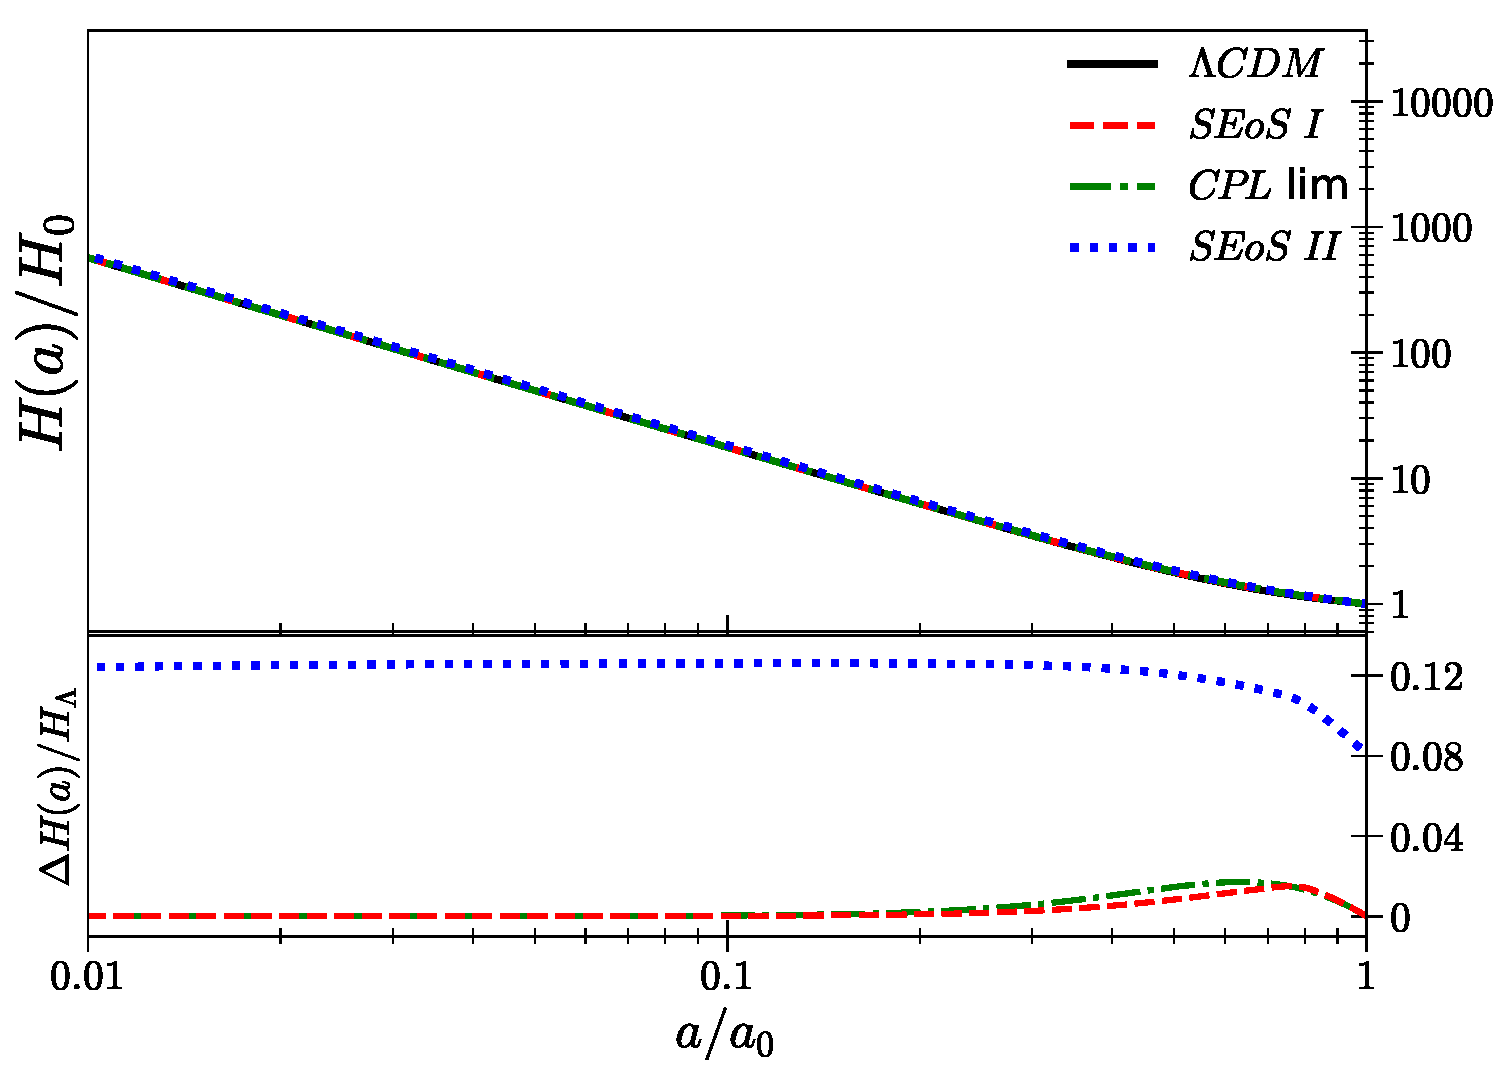
\includegraphics[width=0.6\textwidth,angle=0]{./plots/H_of_a_4_models_ratio.pdf}
\caption{\label{fig:hubble_ratios}{\it Upper panel}: Normalized Hubble expansion rate for the models we consider (listed in Table \ref{table:COLA_models}).  
{\it Bottom panel}: The relative difference w.r.t. $\Lambda$CDM: $\Delta H/H_{\Lambda} \equiv (H/H_{\Lambda} -1)$. Since cases SEoS-I (red dash line), $CPL$-lim (green dotted-dash line), and $\Lambda$CDM (black solid line) share the same values of $H_0$ and $\Omega_{m0}$, they converge to the same $H(z=0)$. CPL-lim has a transition redshift at $z_T=1$, which is larger compared to the one for SEoS case, $z_T=0.28$, and therefore, it shows a departure from $\Lambda CDM$ at a smaller $a/a_0$ value. Since in the SEoS-II case, we have different $H_0$ and also the amount of matter, a discrepancy w.r.t. $\Lambda CDM$ is observed throughout all time scales. This convention in labels for the different models is used throughout the Figures.} 
\label{figure:hubble}
\end{figure}

\begin{figure*}
     \centering
     \begin{tabular}{cc}
        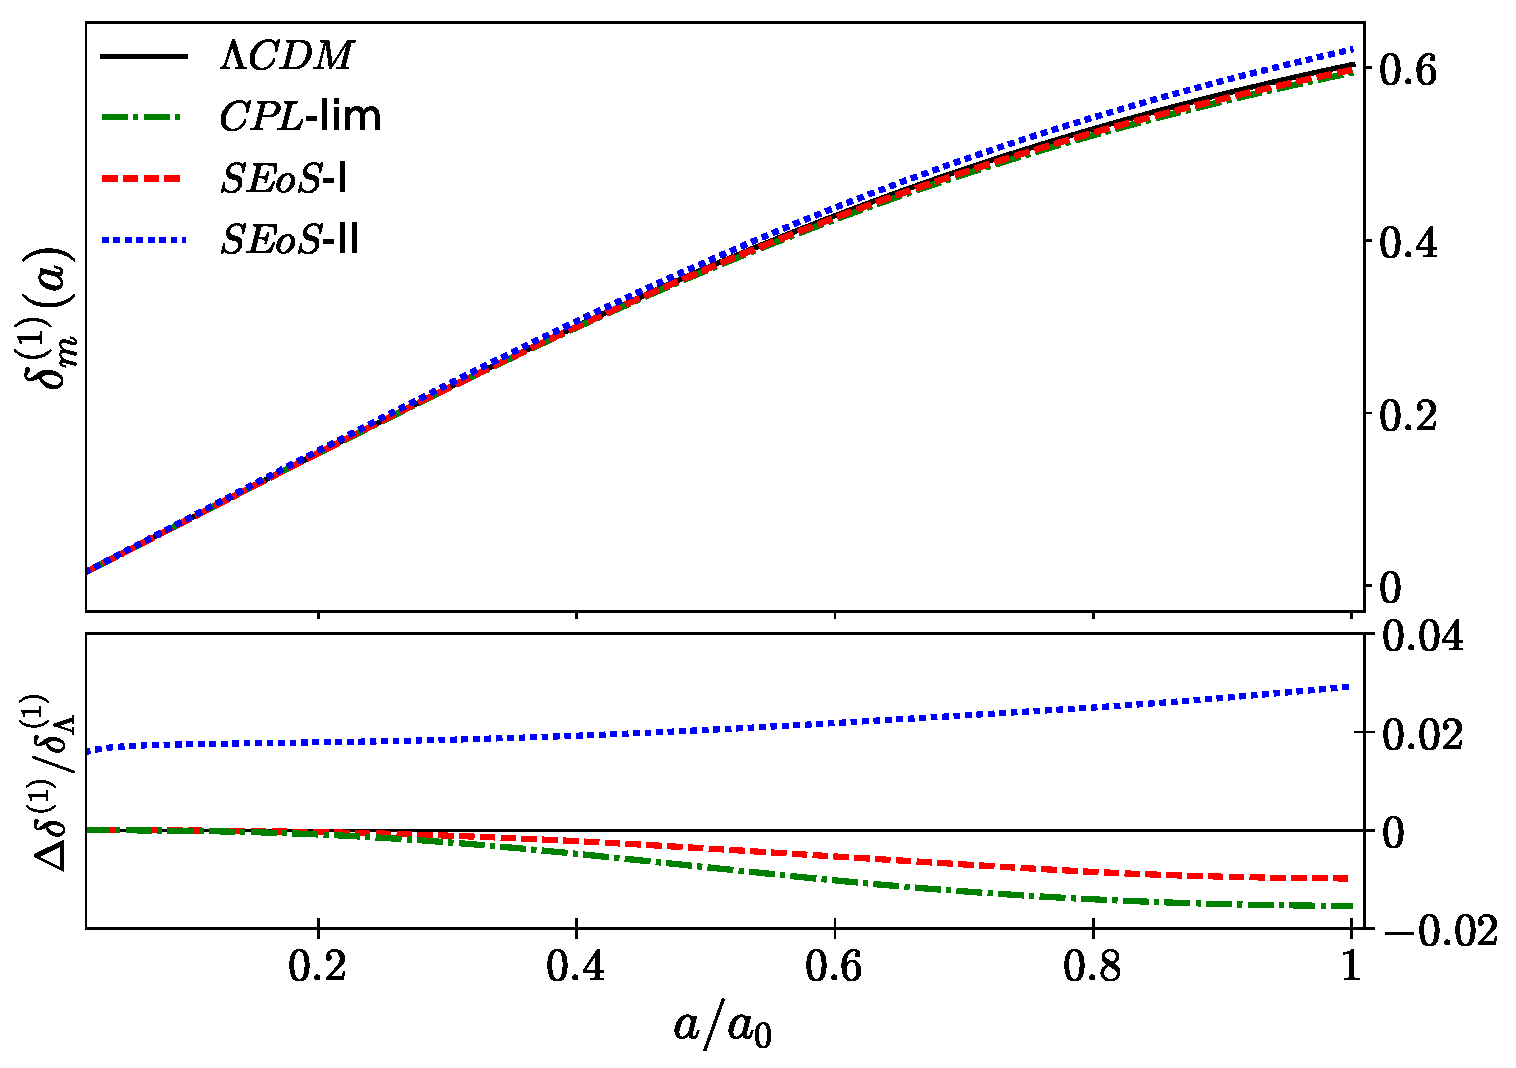
\includegraphics[width=0.49\textwidth,angle=0]{./plots/d1m_4models_ratio_linlin}   
        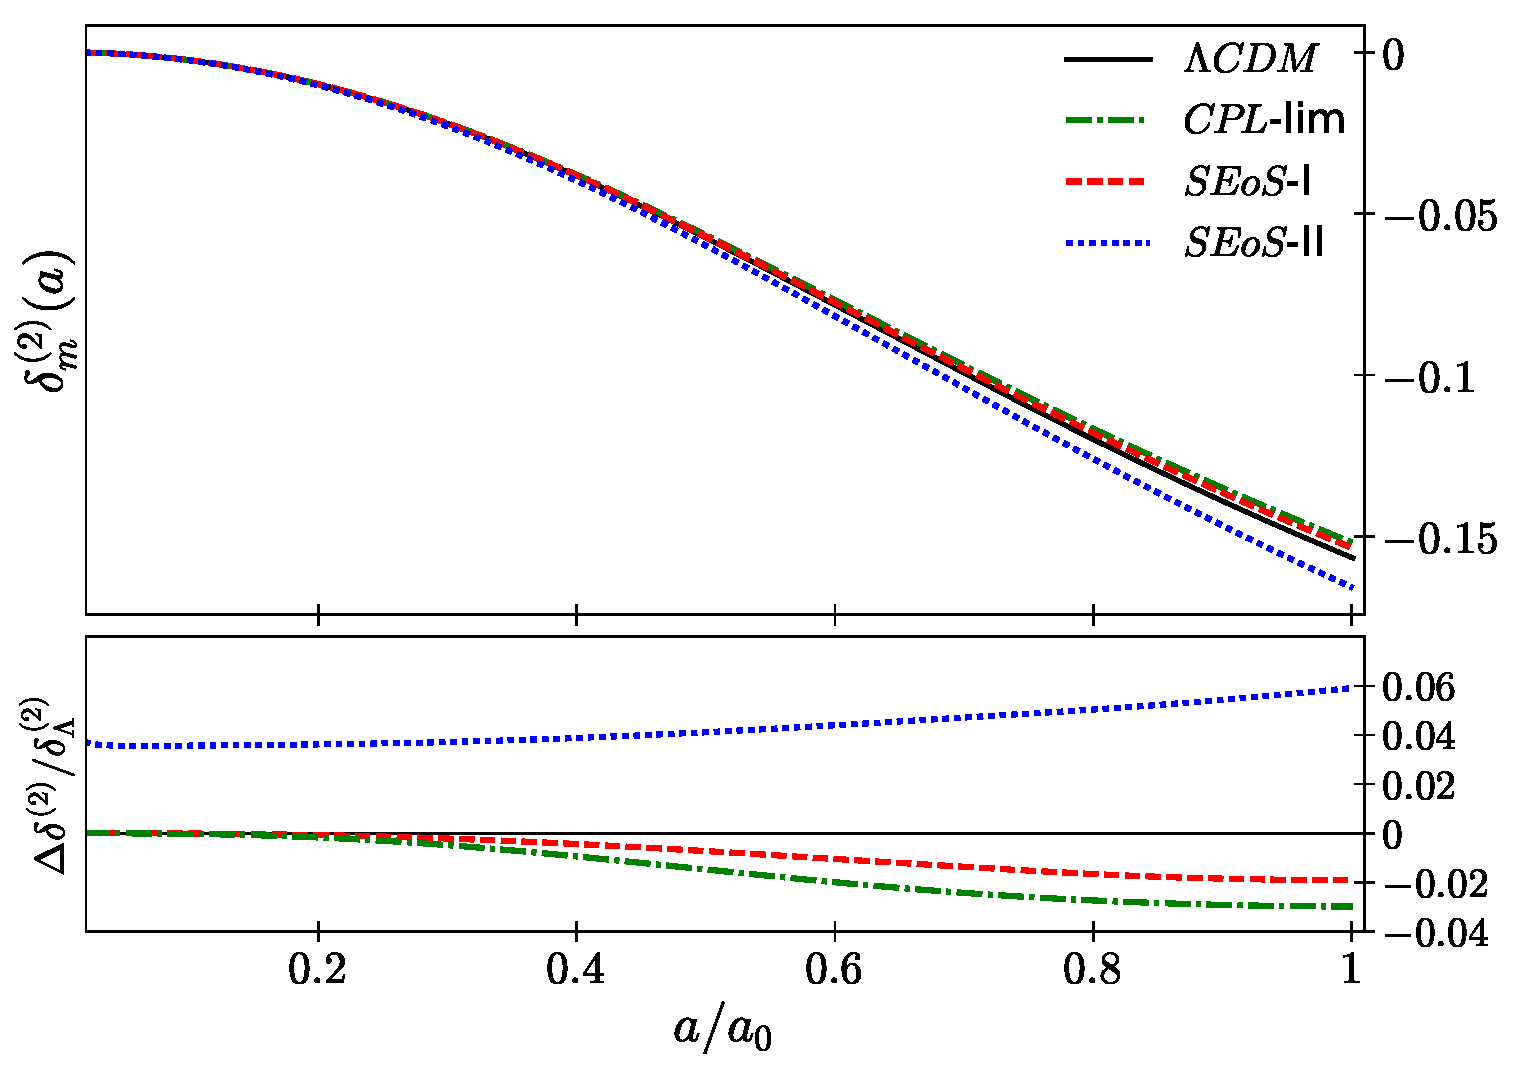
\includegraphics[width=0.49\textwidth,angle=0]{./plots/d2m_4models_ratio_linlin} \\

     \end{tabular}

\caption{%{\it Upper panels:} 
Evolution of the dark matter density contrast at first $\delta_m^{(1)}(a)$ (left panel), and second-order, $\delta_m^{(2)}(a)$ (right panel) for the models considered. The relative differences w.r.t. to $\Lambda$CDM are shown in their respective bottom panels. The case SEoS-I deviates less from $\Lambda$CDM, followed by CPL-lim and SEoS-II. 
}
\label{fig:deltas}
%\end{center}
\end{figure*}

\label{sec:linear}


\begin{figure*}
     \centering
     \begin{tabular}{cc}
        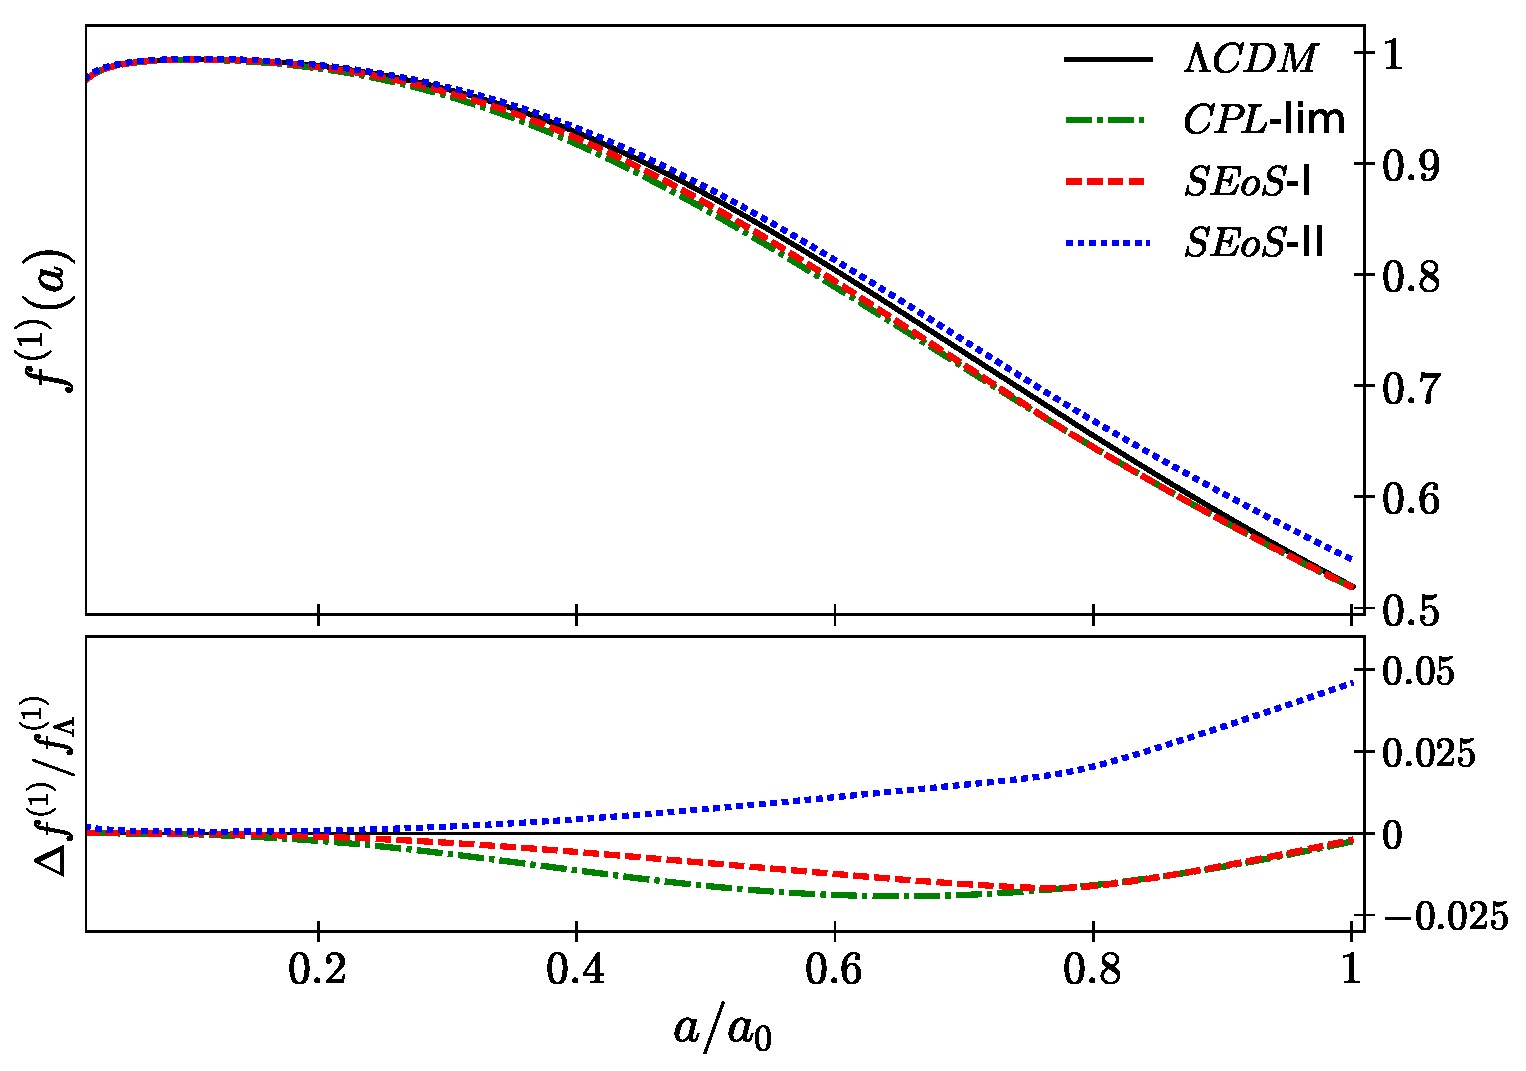
\includegraphics[width=0.5\textwidth,angle=0]{./plots/f1_4models_ratio_linlin}   
        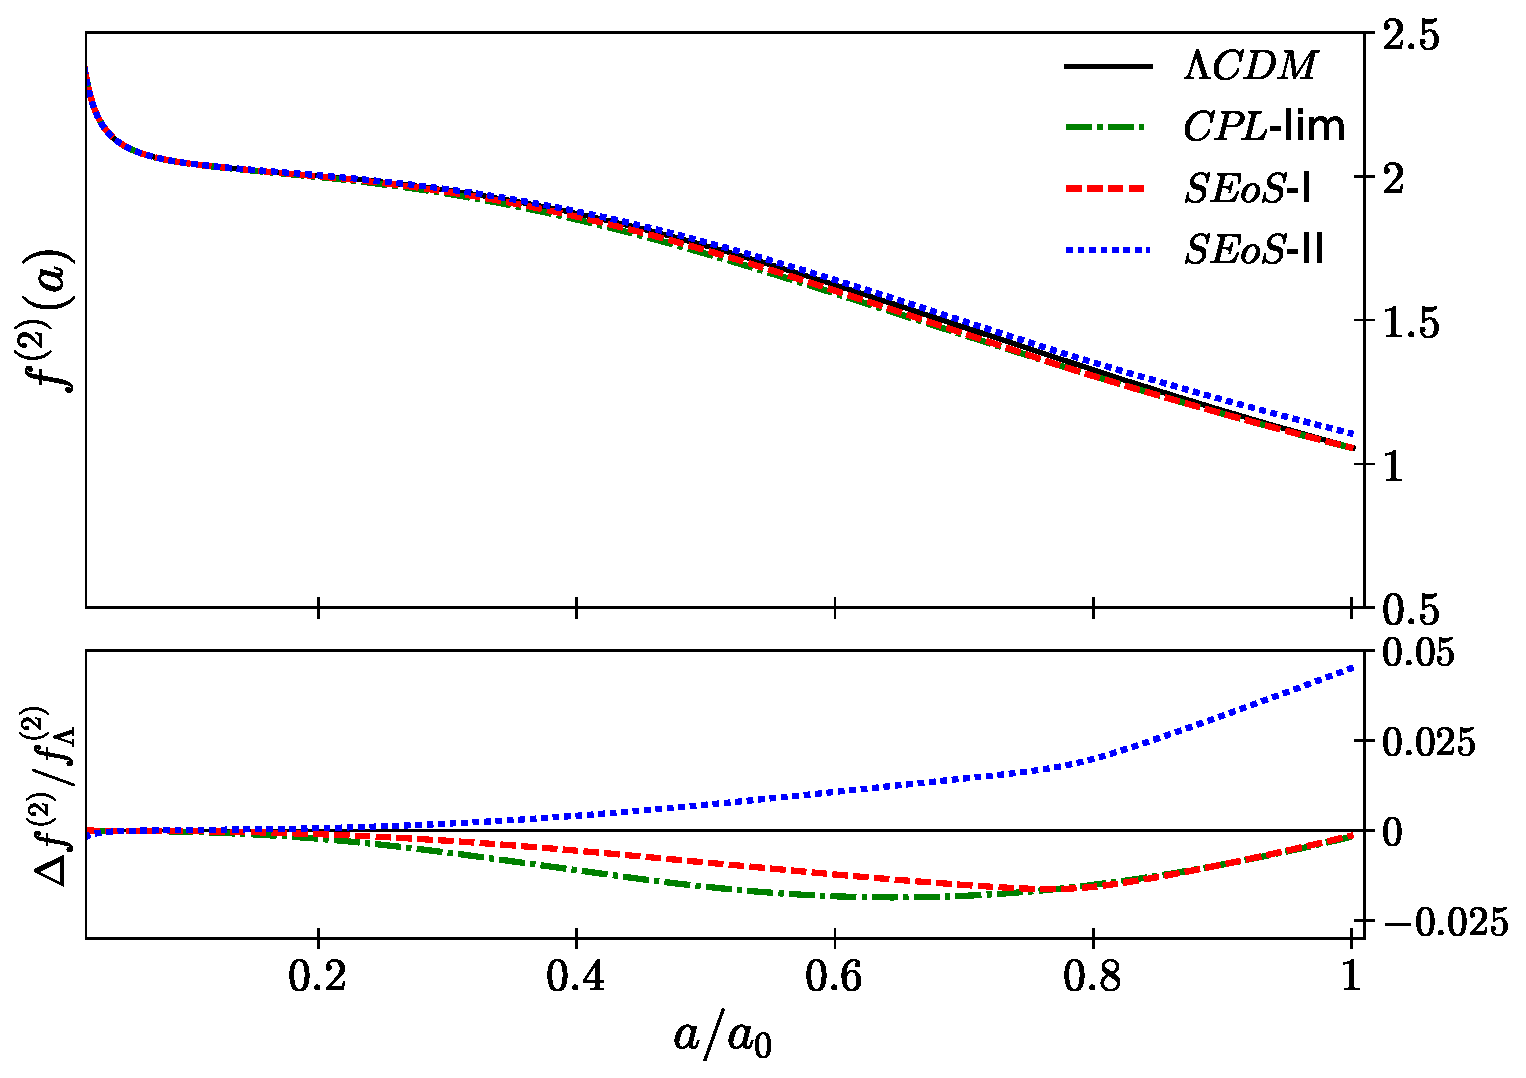
\includegraphics[width=0.5\textwidth,angle=0]{./plots/f2_4models_ratio_linlin} \\

     \end{tabular}

\caption{Evolution of the growth function at first, $f^{(1)}(a)$, and second-order, $f^{(2)}(a)$,  for the models we considered in upper-left and upper-right panels, respectively. The relative differences w.r.t. to $\Lambda$CDM are showing in the bottom panels. The $SEoS$-II model has comparatively higher growth factor in both orders at low redshift, implying faster growing mode then other models. 
}
\label{fig:f_growth}
% \end{center}
\end{figure*}

%%%%%%%%%%%%%%%%%%%%%%%
\subsection{Matter Perturbation Theory}

The evolution of large scale structure is understood to some extent by studying the linear dark matter perturbation theory \cite{Ma:2011nc, Bernardeau:2001qr}. 
Under the assumption that DE remains homogeneously distributed in all scales of our universe, i.e.,  no clustering in the DE component, $\delta \rho_{DE}= 0$, the evolution of the matter density contrast, $\delta_{m} = \frac{\rho_m}{\bar{\rho}_{m}}-1$ up to first and second-order is given by:

\begin{eqnarray}
a^2 \frac{d^2\delta_m^{(1)}}{da^2}+\frac{3}{2}\left(2- w(a)\Omega_{DE}(a)\right)\frac{d\delta_m^{(1)}}{da} -\frac{3}{2}\Omega_m(a)\delta_m^{(1)}(a) = 0,\label{eq:2lptDE1} \\
a^2 \frac{d^2\delta_m^{(2)}}{da^2}+\frac{3}{2}\left(2-w(a)\Omega_{DE}(a)\right)\frac{d\delta_m^{(2)}}{da} -\frac{3}{2}\Omega_m(a)\delta_m^{(2)}(a)= -\frac{3}{2}\Omega_m(a)\left[\delta_m^{(1)}(a)\right]^2 ,
\label{eq:2lptDE2}
\end{eqnarray}
%
where $\Omega_m(a) = \frac{H_{0}^2\Omega_{m0}a^{-3}}{H(a)^2}$ and $\Omega_{DE}(a) =  \frac{H_{0}^2(1-\Omega_{m0})F(a)}{H(a)^2}$. 
%
These coupled differential equations are solved by applying the initial conditions at a time around the recombination epoch, $a_{ini} \approx 0.001$, when the universe was in a matter dominated era, $\Omega_{m} = 1$ (known as ``Einstein-de Sitter'' epoch). In that phase, $\delta^{(1)}_{m}(a)$ evolves linearly with the scale factor and hence we set $\delta_{m}^{(1)}(a_{ini})=a_{ini}$ and  $d\delta_{m}^{(1)}/da(a) = 1$ at $a= a_{ini}$. Likewise, $\delta^{(2)}_{m}(a) \sim -3/7 a^2$ and  $d\delta_{m}^{(2)}/da(a) \sim a $ at $a= a_{ini}$.  


Figure (\ref{fig:deltas}) shows the evolution history of $\delta_{m}^{(1)}$ and $\delta_{m}^{(2)}$ obtained from the above equations. The relative difference w.r.t. $\Lambda$CDM is shown in the respective lower panels.
%
The slight difference in their expansion history, compared to $\Lambda$CDM, makes SEoS-I and CPL-lim models to show lower values in their matter density contrasts w.r.t. $\Lambda$CDM.
%
This is demonstrated in Figure (\ref{fig:deltas}), where we observe a comparatively lower matter density contrasts evolution for both SEoS-I and CPL-lim. For SEoS-I we have differences of $\sim 1\%$ and $\sim 2\%$ in $\delta_{m}^{(1)}$ and $\delta_{m}^{(2)}$, respectively, at $z=0$.% w.r.t. $\Lambda$CDM
% 
The deviation starts to grow around $z \sim 4$ in both cases. In CPL-lim, a deviation reaches to $\sim 1.5\%$ in $\delta_{m}^{(1)}$ and $\sim 3\%$ in $\delta_{m}^{(2)}$ at the same redshift. 
%
However, we do not observe any signatures that can manifest the effect of the steep transition in DE density field in these linear perturbation theory studies. 

In the case of SEoS-II, even though the Hubble expansion rate is higher compared to $\Lambda$CDM, it corresponds to a model with higher matter content, which implies that the DE epoch starts later. Subsequently, the matter density contrast grows faster. % in such scenario.
Therefore, $\delta_{m}^{(1,2)}$  show more significant differences and a faster growth rate over the other cases. 
As expected, the deviation of $\sim 5\%$ is found in $\delta_{m}^{(1,2)}$ at $a = 1$ in SEoS-II. We thus speculate that the possibility of distinguishing between these dynamical DE models from $\Lambda$CDM is around $3-6\%$ via the second-order perturbation theory. %which is qualitatively low while considering the current galaxies surveys precision.

 
To quantify the speed of growth of structure under the cosmological scenarios considered here, we report the logarithmic growth function at first and second order, $f^{(1,2)}\equiv\frac{d\ln\delta_m^{(1,2)}(a)}{d\ln a}$, in Figure \ref{fig:f_growth}. These quantities relate the matter density to velocity dispersion. Figure (\ref{fig:f_growth}) shows that SEoS-I and CPL-lim have comparatively slower growth rates than $\Lambda$CDM in both orders. The growth rate of structures in SEoS-I and CPL-lim models, compared to $\Lambda$CDM, have some specific trends decreasing the rate up to a certain scale and then start to increase until they reach at the same rate as in $\Lambda$CDM. The SEoS-I case turns out to be the closest one to $\Lambda$CDM and SEoS-II has the fastest growing rate over other models. We do expect to observe some effect in the non-linear regime of structure formation as well.

We also fitted $f^{(1,2)}$ for all models using the known fitting formula proposed in \cite{Wang:1998gt} that define $f^{(1,2)}$ as $f^{(1)}=\Omega_m(a)^{\gamma_1}$ and $f^{(2)}= b\times\Omega_m(a)^{\gamma_2}$ with the growth indexes: $\gamma_{1}$, $\gamma_{2}$ and the amplitude parameter, $b$.
The best-fitted values of $\gamma_{1}$, $\gamma_{2}$ and $b$ for all models are listed in table \ref{table:COLA_models}. 
Following \cite{Bouchet1994}, we set $\gamma_1=6/11$, $\gamma_2=0.55$ and $ b=1$ for the $\Lambda$CDM model.

%The accuracy of this fit was examined and found to be within $\sim 0.02\%$ difference between the fitting and numerical values.
%
%Comparing our fitted functions with that of numerically evaluated values from the equations (\ref{eq:2lptDE1}) and (\ref{eq:2lptDE2}), we find a discrepancy of $\sim 0.1 \%$ in $f^{(1)}$, and $f^{(2)}$ solutions, respectively.

%

\section{N-body Simulation: Non-linear Evolution}
\label{sec:nonlinear}

\begin{table*}
	\begin{center}
		\begin{tabular}{l l c c c c c c c c c c}
		%	\hline
		%	\multicolumn{1}{c}{$\La$CDM}\\
			\hline 
			 Model & Alias &$w_0$ & $w_i$ & $q$ & $z_T$ & $\Omega_{m0}$ & $H_0$ & $n_{s}$ &
			 $\gamma_1$ & $b$ & $\gamma_2$ \\
			 \hline \hline 
			$\Lambda CDM$ & $\Lambda CDM$ & -1 & 0 & 0 & 0 & 0.3089 & 67.74 & 0.9667 & 5/9 & 2 & 6/11\\
			\hline
			SEoS  & SEoS-I & -0.92 & -0.99 & 9.98 & 0.28 & 0.3089 & 67.74 & 0.9667 & 0.5527 & 2.0743 & 0.5912\\
			CPL  & CPL lim & -0.92 & -0.99 & 1 & 1 & 0.3089 & 67.74 & 0.9667 & 0.5535 & 2.0751  & 0.5927\\
		\hline
			SEoS & SEoS-II & -0.92 & -0.99 & 9.98 & 0.28 & 0.3340 & 73.22 & 0.9667 & 0.5533 & 2.0859 & 0.5936\\
			\hline %\hline
		\end{tabular}
		\caption{Cosmological and model parameters specification. $\gamma_1$, $\gamma_2$, and $b$, refer to the best fit values found using the fitting formulae for the logarithmic growth functions: $f^{(1)}=\Omega_m^{\gamma_1}$, and $f^{(2)}=b \Omega_m^{\gamma_2}$ \cite{Wang:1998gt}.} 
		\label{table:COLA_models}
	\end{center}
\end{table*}


%____TABLE____________________________________
\begin{table*}
\centering
\begin{tabular}{c|c|c}
\hline
parameter & definition & value \\
\hline
\hline
%$\sigma_{8}$ & r.m.s. linear density fluctuation & $0.8159$ \\
%\hline
$L_{\rm box}$ & simulation box size & 1024~$h^{-1}$Mpc\\
$N_{\rm p}$ & simulation particle number & $1024^3$\\
$N_{\rm Mesh}$ & FFT Mesh & $1024^3$\\
%$m_{\rm p}$ & simulation particle mass & $7.78\times 10^{10}h^{-1}M_{\odot}$\\
$z_{ini}$ & Initial redshift & 49\\
$n_{step}$ & Time steps & 200\\
$ z_{\rm out}$ & Snapshots out at $z$ & $ 0, 0.1, 0.28, 0.56, 1, 1.5, 2, 2.3, 19 $\\
$ N_{\rm run}$ & Number of run & 5 \\
\hline
\end{tabular}
\caption{Specifications of the N-body simulations.}
\label{table:simulation_COLA}
\end{table*}
%____TABLE____________________________________

A way of understanding the structure formation of our Universe in the non-linear regime is by following the formation and distribution of DM halos. This can be done through the full N-body DM simulations. However, in order to achieve a reasonable approximation of the structure formation at large and small scales, the N-body codes need to run numerous time-steps with a fair amount of computational resources.


For our studies we use the COmoving Lagrangian Acceleration (COLA) method\cite{Tassev:2013pn} by modifying the publicly available particle mesh based  N-body code called L-PICOLA\cite{Howlett:2015hfa}. With this N-body DM simulation  we study the cosmological structure formation under the dynamical DE models described in section \ref{sec:background}. 

%we modify the publicly available N-body DM simulation so-called the COmoving Lagrangian Acceleration method\cite{Tassev:2013pn}, particularly L-PICOLA\cite{Howlett:2015hfa} for simulating the cosmological structure formation under the dynamical DE models described in section \ref{sec:background}. 
This scheme has the advantage of accurately recovering the large scale structures (LSS) in few time steps with less usage of computational resources. It is also able to accurately trace the small scales  thanks to the implementation of Lagrangian perturbation theory (LPT), which allows to capture the large scale dynamics directly via the linear growth factors. Note that this makes the code three times faster in comparison to the standard N-body code by enabling it to take larger time steps. 

 
 %This comes from the fact that LSS ($> 100 {\rm Mpc~h^{-1}}$) is well estimated by the Lagrangian perturbation theory. 
 
 %The first and second-order dark matter perturbation solutions are used the COLA code and the small scales are left to be computed by the full N-body method.  
%Due to the fact that the large scale structures ($> 100 {\rm Mpc~h^{-1}}$) can be estimated well by the Lagrangian perturbation theory,  the first and second-order dark matter perturbation solutions are being used in the COLA code and the small scales are left to be computed by the full N-body method. 
%This makes the code 3 times faster in comparison to the standard N-body codes by enabling it to take larger time steps. 
In the following subsection, we briefly describe the COLA method and the Lagrangian perturbation theory employed in the code.

%Basically, in the N-body simulation, the time integration for the large scales is done by solving the linear growth factor but with a few time-steps with an N-body code will provide a wrong clustering for the large-scale.
%For more details we refer to \cite{Tassev:2013pn} and references therein.
%\subsection{2LPT METHOD}

\subsection{COLA Method}

%Previous study has shown that different models predict the differences mainly on small scales ($r < 1 h^{-1}Mpc$) which arguing that an accurate clustering measurements on the small scales can provide significant constraints on the Dark energy or modified gravity models. 

The cold dark matter N-body simulations are governed by a system of equations conformed by the equation of motion and the Poisson equation:
\begin{equation}
\frac{d^2 {\bf x}}{d\tau^2} = - {\bf \nabla} \Phi_{N},
\label{eq:geodesic}
\end{equation}
\begin{equation}
\nabla^2\Phi_{N} = 4 \pi G {\bar{\rho}_{m}}a^4 \delta_{m},   
\label{eq:poisson1}
\end{equation}
where $d\tau = \frac{dt}{a}$ represent the conformal time, $\delta_{m}=\frac{\rho_{m}}{\bar{\rho}_{m}}-1$, the  matter density contrast in the particle positions $\bf{x}$, and $\Phi_N$ is the Newtonian potential.

However, in the COLA approach rather then solving the Newtonian potential for the particle positions, $\vec{x}$, one solves for the perturbation around the path $\vec{x}_{LPT}$ provided by the second-order Lagrangian perturbation theory, i.e., $\vec{x} = \vec{\delta x}+\vec{x}_{LPT}$. Thus, the equation of motion takes the form:
\begin{equation}
\frac{d^2 \vec{\delta x}}{d\tau^2} = - \vec{\nabla} \Phi_{N} - \frac{d^2\vec{x}_{LPT}}{d\tau^2}.
\end{equation}
This equation is solved as a system of coupled equations: 
\begin{equation}
\frac{d\vec{\delta}v}{d\tau} = -\vec{\nabla}\Phi_{N} - \frac{d^2\vec{x}_{LPT}}{d\tau^2},
\end{equation}
\begin{equation}
\frac{d\vec{\delta x}}{d\tau} = \vec{\delta v},   
\end{equation}
which will track the large scale evolution according to the Lagrangian perturbation theory.
\subsubsection{2LPT}
According to the Lagrangian perturbation theory (LPT) \cite{Bernardeau:2001qr}, the position of a particle in Eulerian space, $\bf{x}$, is described by its initial Lagrangian position, $\bf{q}$, and a displacement field of the particle, $\bf{\Psi}$, through the mapping:  
\begin{equation}
\bf{x}(q,\tau) = \bf{q}+\bf{\Psi}(\bf{q},\tau),
\label{eq:LPT_position}
\end{equation}
and the equation of motion \eqref{eq:geodesic} as given by
\begin{equation}
\frac{d^2 \bf{\Psi}}{d\tau^2} + \mathcal{H}(\tau)\frac{d\bf{\Psi}}{d\tau} +{\bf \nabla}\Phi_N = 0.
\label{eq:geodesic2}
\end{equation}
Hence, the Poisson equation \eqref{eq:poisson1} can be written as
\begin{equation}
{\bf \nabla_{x}} \left( \frac{d^2 \bf{\Psi}}{d\tau} + \mathcal{H}(\tau)\frac{d\bf{\Psi}}{d\tau}\right) = \nabla^2\Phi_N = - \frac{3}{2}\Omega_{m0}\mathcal{H}(\tau) \delta_{m}(\tau)= -\kappa \delta_{m},
\label{eq:poisson}
\end{equation}
where $\kappa = \frac{3}{2}\Omega_{m0}\mathcal{H}(\tau)$, and $\mathcal{H}$ is the conformal Hubble expansion rate. 

In LPT, the above equation is generally solved by perturbatively expanding the displacement vector as $\bf{\Psi} = \bf{\Psi}^{(1)} +\bf{\Psi}^{(2)}+ ...$, where $\bf{\Psi}$ represents a curl-free gradient of a scalar field, $\phi^{(i)}$, $\bf{\Psi}^{(i)} = \bf{\nabla}_{q}\phi^{(i)}$.
Similarly, expanding the density contrast in a perturbative series we have $\delta_m(x) = \delta_m^{(1)}+ \delta_m^{(2)}+ ... = J^{-1}-1$, with $J = \rm{Det}(\delta_{ij} +{\bf{\Psi}}_{i,j})$, the Jacobian of the transformation. Now  we can equate each order and obtain:
%$\delta = \delta^{(1)}+ \delta^{(2)}+ ... = \left|\frac{\partial(x)}{\partial(q)}\right|^{-1} - 1 = J^{-1}-1$
\begin{equation}
\delta_{m}^{(1)} = - \bf{\Psi}^{(1)}_{i,i},
\end{equation}
\begin{equation}
\delta_{m}^{(2)} = - \bf{\Psi}^{(2)}_{i,i} +\frac{1}{2}\left((\bf{\Psi}^{(1)}_{i,i})^2 +(\bf{\Psi}^{(1)}_{i,j})^2\right),
\label{eq:delta2}
\end{equation}
where $\bf{\Psi}_{i,j}=\partial \bf{\Psi}_{i}/\partial q_{j}$, and the divergence w.r.t. $x$ is changed to $q$ via the Jacobian transformation: $\nabla_{x_i} =(\delta_{ij}+{\bf{\Psi}}_{i,j})^{-1}\nabla_{\bf q_j}$. 
At first order, we have from equation \eqref{eq:poisson}:
\begin{equation}
\frac{d^2 {\bf\Psi}^{(1)}_{i,i}({\bf q},\tau)}{d\tau^2} = -\kappa \delta_{m}^{(1)}({\bf q},\tau),    
\end{equation}
which is equivalent to 
\begin{equation}
\left(\frac{d^2}{d\tau^2}-\kappa\right) \nabla^2 \phi^{(1)}({\bf q},\tau) =0,
\label{eq:1st_LPT}
\end{equation}
%
where $\phi^{(1)}({\bf q},\tau)$ is factorized into the time-dependent normalized growth factor, $D^{(1)}(\tau)$ multiplied by $\phi^{(1)}({\bf q},\tau_{in})$, the initial condition field coming from $\delta^{(1)}({\bf q},\tau_{in})$. Thus, the growth factor $D^{(1)}(\tau)$ follows the equation:
\begin{equation}
\left(\frac{d^2}{d\tau^2}-\kappa\right) D^{(1)} =0,
\end{equation}
%
and it can  be solved easily by assuming the initial conditions according to the growing mode of the matter dominated ``Einstein de-Sitter'' Universe, $D_{in}^{(1)} =1$, and $\frac{dD^{(1)}_{in}}{d\tau}=\left(\frac{1}{a}\frac{da}{d\tau}\right)_{\tau =\tau_{in}}$. 

Note that it is the same solution we obtained from eq. \eqref{eq:2lptDE1}.  
So, the first-order displacement field at any time is simply given by ${\bf \Psi}^{(1)}(q,\tau)= D^{(1)}(\tau){\bf \Psi}^{(1)}(q,\tau_{i})$, i.e., once the displacement field at the initial time is computed in the simulation,  $\bf{\Psi}^{(1)}$, we can track it at any later time simply multiplying it by the growth factor.
Similarly, using the equations \eqref{eq:delta2} and \eqref{eq:poisson}, the second-order Lagrangian perturbation takes the form of 
\begin{equation}
\left(\frac{d^2}{d\tau^2} -  \kappa \right)\nabla^2\phi^{(2)} = -\frac{\kappa}{2}\left[(\nabla^2\phi^{(1)})^2 - (\nabla_{i}\nabla_{j}\phi^{(1)})^2\right],
\label{eq:2nd_LPT}
\end{equation}
with $\phi^{(2)}(q,\tau) = D^{(2)}(\tau)\phi^{(2)}(q,\tau_{in})$, and where the second-order growth factor $D^{(2)}$ satisfies 
\begin{equation}
\frac{d^2 D^{(2)}}{d\tau^2}-\kappa D^{(2)} = -\kappa (D^{(1)})^2.
\label{eq:D2}
\end{equation}
%
We again provide the initial conditions according to an Einstein-de Sitter Universe: $D^{(2)}_{in} = -\frac{3}{7}$ and $\frac{dD_{in}^{(2)}}{d\tau} = - \frac{6}{7}\left(\frac{1}{a}\frac{da}{d\tau}\right)_{in}$, and the solution is nothing but the solution of \eqref{eq:2lptDE2}. The second-order initial field, $\phi^{(2)}(q,\tau_{in})$, is given by
 \begin{equation}
\nabla^{2}\phi^{(2)} = \frac{1}{2}\left[(\nabla^2\phi^{(1)})^2 - (\nabla_{i}\nabla_{j}\phi^{(1)})^2\right]. 
 \end{equation}
Hence, in LPT, the equation \eqref{eq:LPT_position} reduces to 
\begin{equation}
{\bf x} = {\bf q}- D^{(1)}{\bf\nabla_{q}}\phi^{(1)}+D^{(2)}{\bf \nabla_q}\phi^{(2)}, 
\label{eq:LPT_position_pot}
\end{equation}
and the velocity field, $v$ is governed by
\begin{equation}
{\bf v} =\frac{d{\bf x}}{d\tau} = -D^{(1)}f^{(1)}\mathcal{H} {\bf \nabla_{q}}\phi^{(1)}+D^{(2)}f^{(2)}\mathcal{H}{\bf \nabla_{q}}\phi^{(2)},
\end{equation}
where $f^{(1,2)}$ represent the growth rate functions $f^{(1,2)} = \frac{d\ln D^{(1,2)}}{d\ln a}$.

For our dynamical DE models, $D^{(1,2)}$ and $f^{(1,2)}$ are provided by solving equations \eqref{eq:2lptDE1} and \eqref{eq:2lptDE2} along with their Hubble expansion rates. The main differences observed among each other and from $\Lambda$CDM have been discussed in subsection (\ref{sec:linear}).

%From Figure \ref{fig:hubble_ratios} we observe that the difference in Hubble rates for the $CPL$-lim and $SEoS$-I models from the $\Lambda CDM$ remain within $\sim 2\%$ throughout all redshifts.    In case of $SEoS$-II model, the deviation reaches up to $\sim 12\%$ starting from the $z=1$ towards higher redshifts.

\subsubsection{COLA Approach}
In the COLA method, the equation of motion is solved in the frame of reference comoving with the particles in Lagrangian space.  
%
After the method is applied, we have the residual displacement, $\Psi_{res}$, where the Zel'dovich and quasi-linear 2LPT displacement fields ($\Psi^{(1)}$ and $\Psi^{(2)}$, respectively) have been subtracted from the full non-linear displacement that each particle experiences.

\begin{equation}
\Psi_{res} = \Psi - D^{(1)}\Psi^{(1)} - D^{(2)}\Psi^{(2)}.    
\end{equation}
Hence, the equation of motion(\ref{eq:geodesic2}) takes the form:
\begin{equation}
T^2[\Psi_{res}] = -\nabla\Phi_{N}- T^2[D^{(1)}]\Psi^{(1)} - T^2[D^{(2)}]\Psi^{(2)} 
\end{equation}
where $T^2[X] = \frac{d^2X}{d\tau^2} +\mathcal{H}\frac{dX}{d\tau}$. The residual displacement, $\Psi_{res}$ is left  to be computed by the usual Particle-Mesh scheme.

For more details about the method implementation and the way the time integration has been discretized on the operator, $T$, we refer the reader to references \cite{Tassev:2015mia, Howlett:2015hfa}. 
%
Note that in the limit of a large number of time-steps, this method recovers the same result as the standard approach for N-body simulations both on the large and small scales.

Thus, in the COLA approach, the run time is directly proportional to the number of time steps we set to run the simulation. Previous studies of the COLA approach have already shown that with ten steps, it converges to the same results as a full-N body simulation with an accuracy of up to $2\%$ for $k = 1h/Mpc$. Hence the convergence rate increases as we increase the number of time steps. Nevertheless, we recall that the goal of our work is not to test the accuracy of the code, but rather to study the effect of dynamical DE models.


%The mass of the particle is determined by 
%$m_{particles} = \frac{\Omega_{m0}\times\rho_{crit}* L^3}{N_{particles}} $

\subsection{Simulation set up}

We follow Planck cosmology \cite{Ade2016}: $\Omega_{m0}=0. 3089$, $h =0.6774$, $n_s=0.9667$, $\sigma_8=0.8159$, and the model parameters are set according to the best fit values from \cite{Jaber:2017bpx}. Specifically, for the CPL-lim we have $w_{0} = -0.92, w_{i} =-0.99, z_{T} =1 =q$ and the SEoS models have $w_{0} =-0.92, w_{i} =-0.99, z_{T}=0.28, q=9.98$. Recall that SEoS-I and SEoS-II models are differentiated by the fact that SEoS-II is run with $\Omega_{m0}=0.334$ and $ h=0.7322$. 

For the N-body simulations we use a box of side length $L_{\rm box}=1024 h^{-1}{\rm Mpc}$ (L1024 in Table \ref{table:simulation_COLA}), $N_{p} = 1024^3$ dark matter particles, and a mesh of $N_{\rm mesh}= 1024$ for FFT calculations.
%The parameters for the N-body simulations are box size $L_{\rm box}=1024 h^{-1}{\rm Mpc}$ (L1024) with $N_{p} = 1024^3$ dark matter particles on a mesh, $N_{\rm mesh}= 1024$. 
These parameters lead to a value for the mass of particles: $m_{part}=8.57198 \times 10^{10}{\rm M_{\odot}}h^{-1}$ for $\Omega_{m0}=0.3089$, and $m_{part}=9.2685 \times 10^{10} {\rm M_{\odot}}h^{-1}$ for $\Omega_{m0} = 0.334$, respectively. 


The initial matter power spectra that we input to the simulations was generated with CAMB \footnote{https://camb.info/}. The initial particles distribution is created using the 2LPTic initial conditions code \cite{Crocce:2006ve} \footnote{http://cosmo.nyu.edu/roman/2LPT/} at the initial redshift of $z_{in}=49$. 
%
Upon the modification of the COLA-code by incorporating the behavior of dynamical DE models, we run the simulation with 200 time-steps between  $z_{in}=49$ and $z=0$, and take several snapshots at different redshift values for each model. To suppress sampling variance on our results, we estimate them by averaging 5 independent realizations, each one run with different random seeds. Our results will be focused at redshifts, $z=0, 0.28 $ and $1$. Keeping in mind that $z=0.28$ and $z = 1$ are the transition points, $z_{T}$, for SEoS models and CPL-lim respectively. 
A summary of the cosmological and simulation parameters is listed in tables (\ref{table:COLA_models}) and (\ref{table:simulation_COLA}). 

\section{Results}
\label{sec:results}
The effect of dynamical dark energy is often studied through the dark matter particles and halo properties. 
Particularly through quantities such as the dark matter power spectrum, velocity power spectrum, halo abundances and halo-clustering at different redshifts. 
For our case, we calculate the matter power spectrum using the SimplePofk code \footnote{http://ascl.net/1110.017} \cite{Colombi2011}, where the density field is estimated using a Cloud-in-Cell mass assignment method on a cubic grid with the same resolution as the Particle-Mesh grid used for the integration of the N-body system. 
The halo catalogs are generated using a publicly available phase-space temporal halo finder called Rockstar \footnote{https://bitbucket.org/gfcstanford/rockstar} \cite{Behroozi2013}. The Rockstar halo-finder is set to find  the halos with a minimum of $20$ particles, which leads to the minimum mass of the halo of $\sim 2 \times 10^{12}{M_{\odot}}h^{-1}$. Later on, we study the effect on the dark matter halos clustering by calculating the two-point correlation function in real space. 
%For this propose we use a publicly available code called CUTE \cite{cutecode}\footnote{https://github.com/damonge/CUTE}. 

\subsection{Non-linear matter power-spectrum} 

\begin{figure*}
     \centering
     \begin{tabular}{cc}
        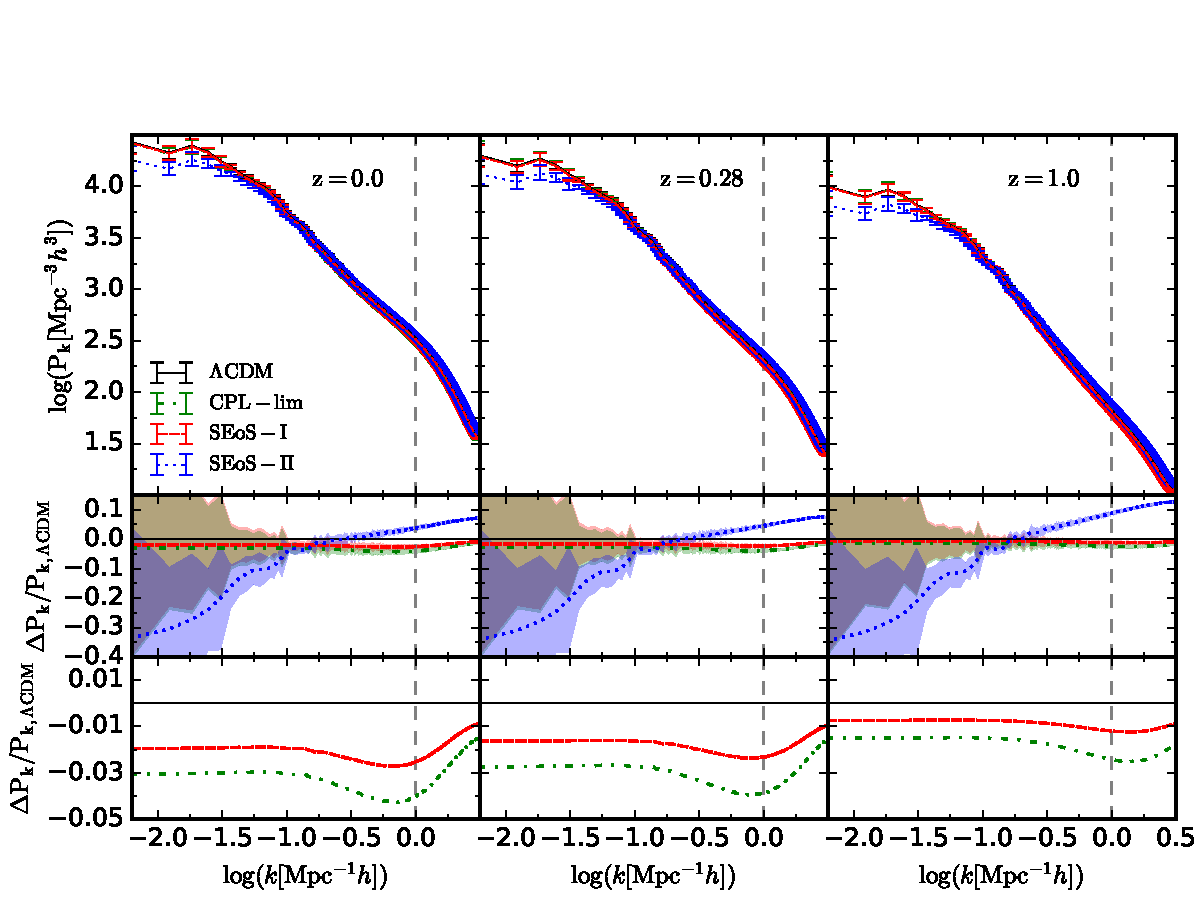
\includegraphics[width=1\textwidth,angle=0]{./plots/power_spectrum_all.pdf}   

 \end{tabular}

\caption{{\it Upper Panels:} The dark matter power spectra for all the models at redshifts: $z = 0, 0.28, 1$. We follow the same color coding to represent the corresponding models as before. {\it Middle panels}: The relative difference of our models w.r.t. $\Lambda$CDM. Shaded regions represent one sigma standard deviation propagated from 5 realizations run with the different random seeds. {\it Lower panels}: Relative differences of SEoS-I and CPL-lim w.r.t. $\Lambda$CDM. The vertical line provides the limit beyond which the $P_{k}$ can not be trusted. 
%Note: The SEoS-I and CPL models show difference less then $\sim 3-4\%$ from $\Lambda$CDM.
}
\label{fig:pk_nonlinear}
%\end{center}
\end{figure*}



\label{sec:pk} 

In Figure (\ref{fig:pk_nonlinear}), the non-linear matter power spectra, $P_{k}(k,z)$ of all models are plotted at  redshifts $z=0$, $0.28 $, and $1.0$. The power spectra are based on the simulation ${\rm L1024}$. In each panel, solid black, green dotted-dash, red dashed, and blue dotted lines correspond to $\Lambda$CDM, SEoS-I, CPL-lim, and SEoS-II models, respectively. The relative differences w.r.t. $\Lambda$CDM for all models are shown in the middle panels. The shaded portions represent the error propagated from the $1\sigma$ standard deviations of 5 realizations, run with the different initial random seeds. The bottom panels highlight the difference between SEoS-I, and CPL-lim from $\Lambda$CDM.  

%Figure (\ref{fig:pk_nonlinear}) show a consistent standard behavior of $P_{k}$ of all models with the variation of redshift.% i.e., $P_{k}$ reduces with the increase of redshift. 
 %From the bottom panels of Figure (\ref{fig:pk_nonlinear}),
The $P_{k}$ of SEoS-I (red dashed) and CPL-lim (blue dotted) show a deficit in power of $\sim 2\%$ and $\sim 3\%$, respectively, throughout all k-scales w.r.t. $\Lambda$CDM, and a slight increase in power at the non-linear regimes that reaches $\sim 3-4\%$ (see bottom panels of Figure (\ref{fig:pk_nonlinear})). Note that the maximum deviation observed in the linear growth $\delta^{(1,2)}$ for these models is within $\sim 2-3\%$ at $z = 0, 0.28, 1$. This points out that the impact of dynamical DE is relatively small both in linear and non-linear regimes.

However, the overall deficits in $P_{k}$ for SEoS-I and CPL-lim highlight the impact that different DE dynamics has in the growth of structure. Explicitly, the effect of having less negative values of $w(z)$ for both SEoS-I and CPL-lim compared to $\Lambda$CDM (for instance: $w_{SEoS-I} =  -0.97$, $w_{CPL-lim} = -0.95$ and $w_{\Lambda}= -1$ at $z = 0.28$), makes the models to evolve with a slightly larger expansion rate, $H(a)$, and therefore to enter the DE-dominated epoch relatively earlier than in $\Lambda$CDM. This results in slowing down the growth of structures as compared to a $\Lambda$CDM universe. 

The trend of a reduction in the  $P_{k}$ amplitude as redshift goes to zero is again showing the effect of DE behavior, as a consequence of their expansion rates. In particular, $2 \%$ and $3 \%$ differences at $z = 0$ reduce to $1 \%$ and $2 \%$ at $z = 1.0$ for SEoS-I and CPL-lim, respectively.

On the other hand, the $P(k)$ of SEoS-II can be understood by recalling the behavior of linear power spectrum, $P_{k,lin}$, of $\Lambda$CDM  for varying $\Omega_{m0}$ and $H_{0}$. For instance, looking at $P_{k,lin}$ of $\Lambda$CDM at $\Omega_{m0} =0.3089$ and $\Omega_{m0}=0.334$ for the same $H_{0}$, we find that $P_{k,lin}$ of $\Omega_{m0}=0.334$ has a deficit in power at low $k$-modes (linear regime), then it increases and peaks in amplitude at high $k$-modes (non-linear regime). The larger the value of $\Omega_{m0}$, the greater deviation we observe in $P_{k,lin}$, depicting the direct proportionality of $P(k)$ with $\Omega_{m0}$ both in linear and non-linear regimes (see Figure \ref{app:Pk_initial}).
Since $H_{0}$ does not change with time, the difference in $P_{k}$ at different redshifts are not effected by $H_{0}$.
%The deviation can go from $\sim 10\%$ deficit in power at $k = 0.001$ upto $\sim 20\%$ enhancement at $k =10$, noting the difference of $8\%$ in $\Omega_{m0}$ (see Figure \ref{app:Pk_initial}). Larger the value of $\Omega_{m0}$, higher the deviation we observed in $P_{k,lin}$, showing the direct proportionality to $\Omega_{m0}$ both in linear and non-linear regimes with the shift in $P_{k}$. % The effect of having a larger value of $H_{0} = 0.7332$ on the $P_{k}$ is more predominant in the non-linear regime. Higher $H_{0}$, larger the deviation we observed in $P_{k}$ when compare with $H_{0} = 0.6774$.  


Even though the effect of DE is manifested in a greater proportion in the linear regime for models SEoS-I and CPL-lim, for SEoS-II we have the conjunction of DE dynamics with the larger value of the amount of matter contained, $\Omega_{m0} = 0.334$. For this large value of $\Omega_{m0}$, the structures formed in denser environments (see $\delta^{(1,2)}$ in Figure (\ref{fig:deltas})), which subsequently led to low values in $P_{k}$ at low $k$-modes. 

%Even though the effect of DE in general is larger at the linear regime over the non-linear one, in case of SEoS-II where the matter contained, $\Omega_{m0} = 0.334$ is much higher then other models including $\Lambda$CDM, i.e., $\Omega_{m0} = 0.3089$, the structures formed in such environments are more dense (see $\delta^{(1,2)}$ in Figure (\ref{fig:deltas})), thus, subsequently leads to low values in $P_{k}$ at low $k$ modes. 
%

Having the values $\Omega_{m0} = 0.334$ and $H_{0} = 0.7332$ results in more clustering at the non-linear regimes. More specifically, our result in Figure (\ref{fig:pk_nonlinear}) shows a difference as large as $\sim 30\%$ at $k= 0.001$ between the SEoS-II model and $\Lambda$CDM, difference that reduces up to $\sim 10\%$ at the non-linear regime (say $k=10$). The slight reduction in power of $P_{k}$ of SEoS-II between $z = 1$ and $z = 0$ on high $k$-modes is due to DE effect that we observe in $H(a)$ (see Figure (\ref{figure:hubble})).


From this analysis we find that the effect of having a steep transition in the DE models does not imprint a sharp signature in the  $P_{k}$, but does affect it due to the overall impact  of DE dynamics.
%is difficult to detect in $P_{k}$ in front of overall impact  of DE.
As expected from the background studies, SEOS-I turns out to be the closest to $\Lambda$CDM, followed by CPL-lim and SEoS-II



\subsection{Two point correlation function}

\begin{figure*}
	\centering
	\begin{tabular}{cc}
		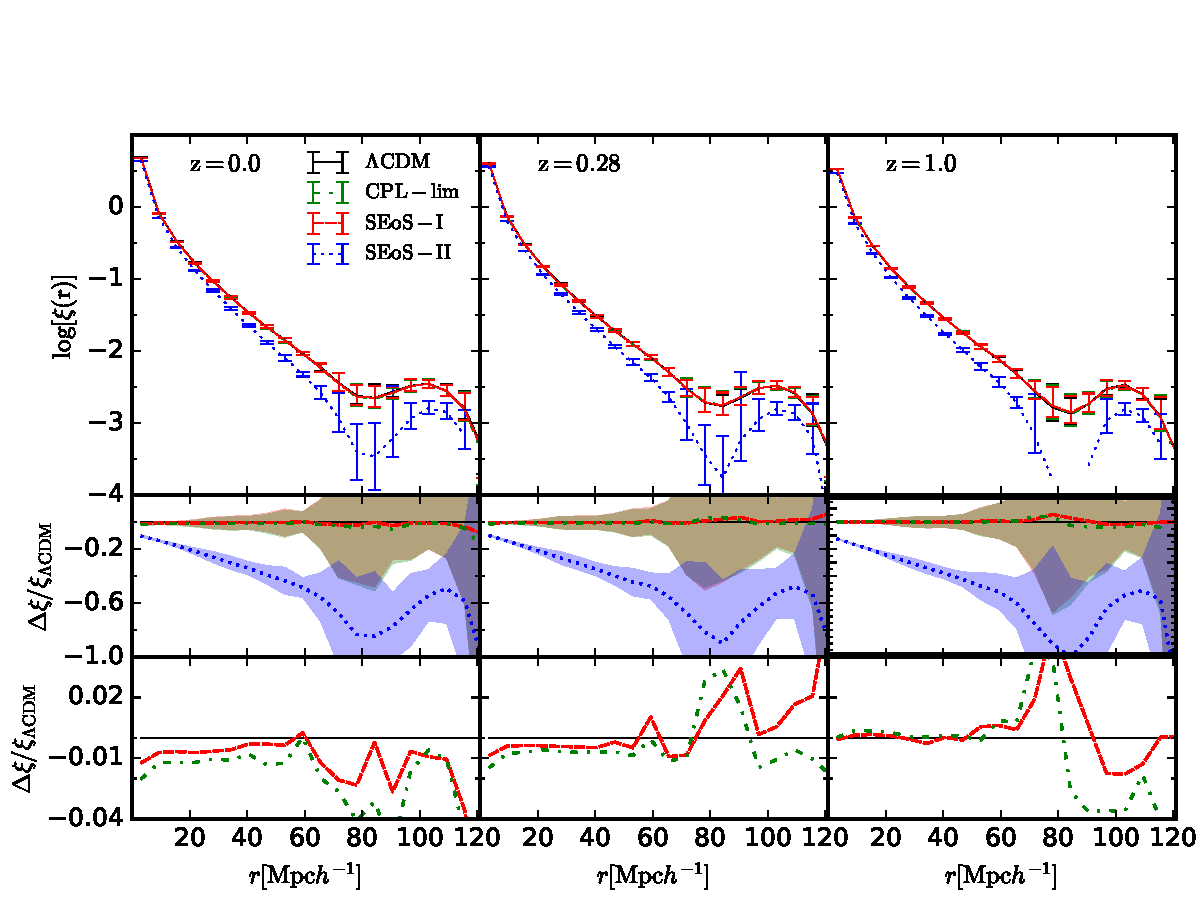
\includegraphics[width=1\textwidth,angle=0]{./plots/2cpf_new.pdf}
		%  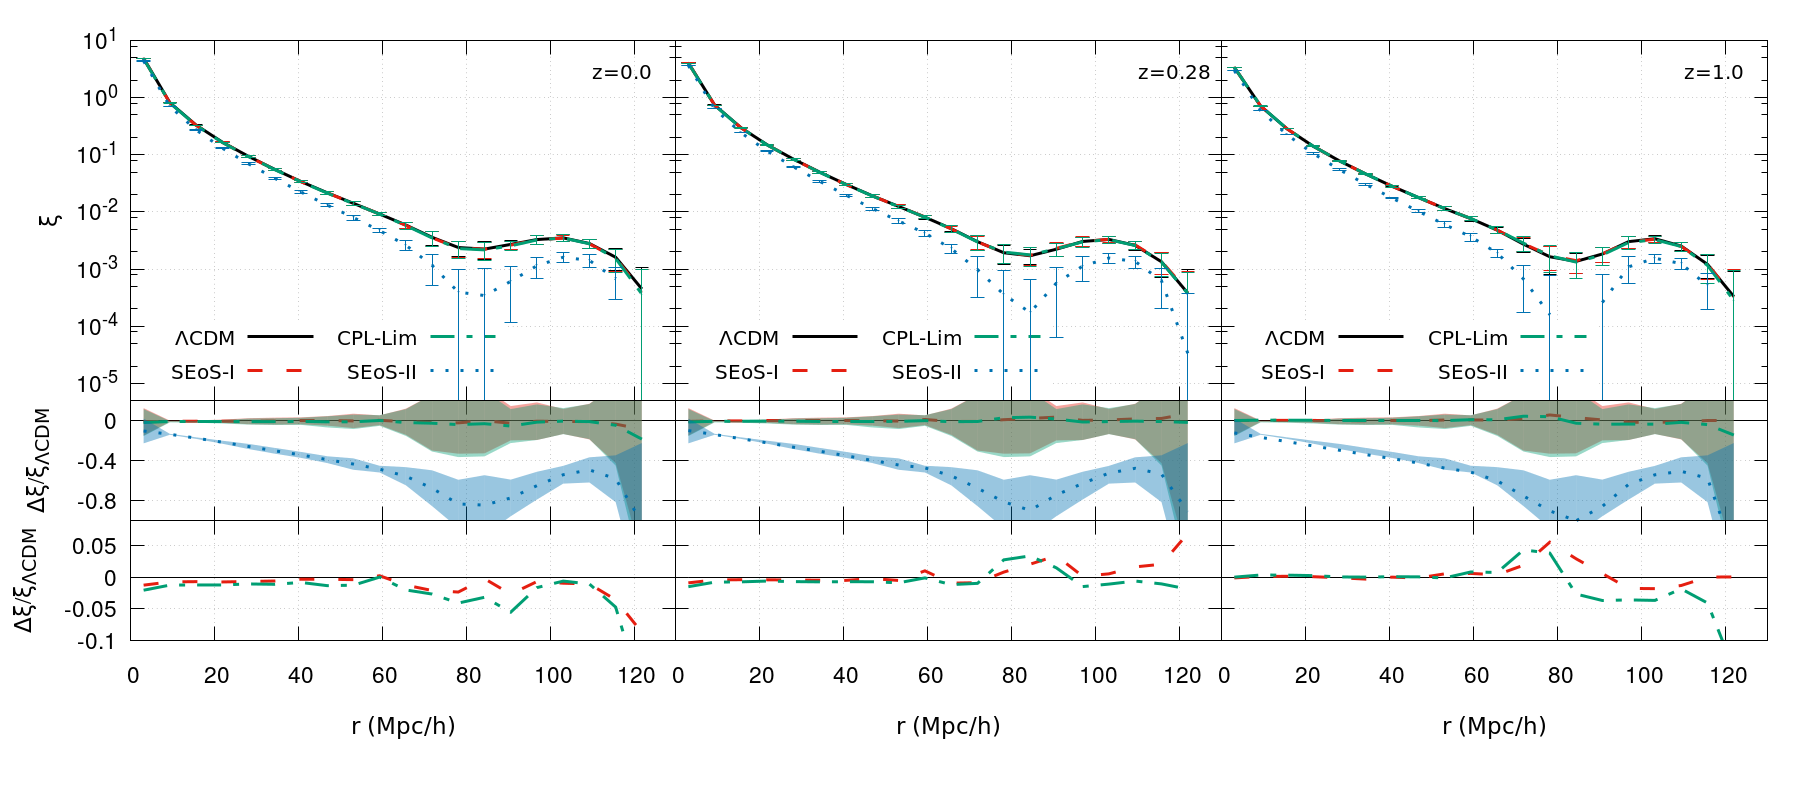
\includegraphics[width=1\textwidth,angle=0]{./plots/HS-50_Prom_2PCF_wZoom_sinr2_halos_Lb1024_}
		%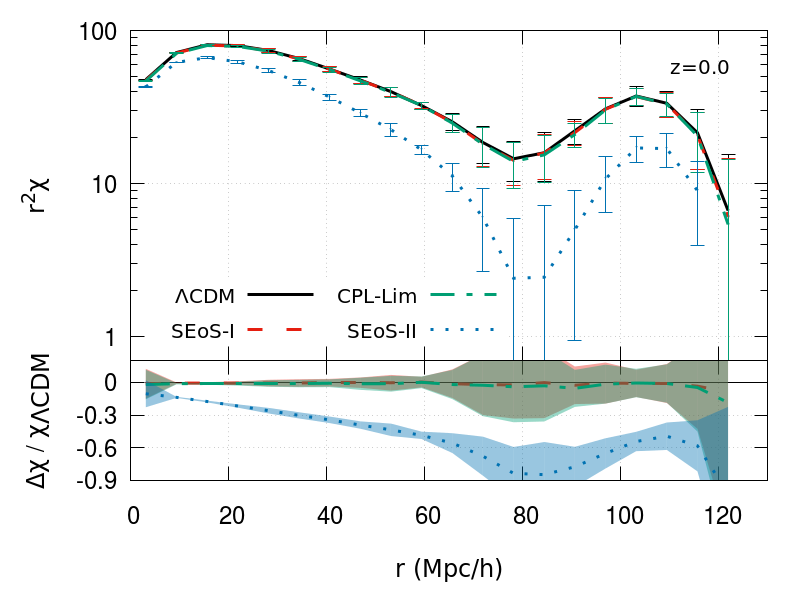
\includegraphics[width=0.33\textwidth,angle=0]{./plots/HS-50_Prom_2PCF_halos_Lb1024_out11}   
		%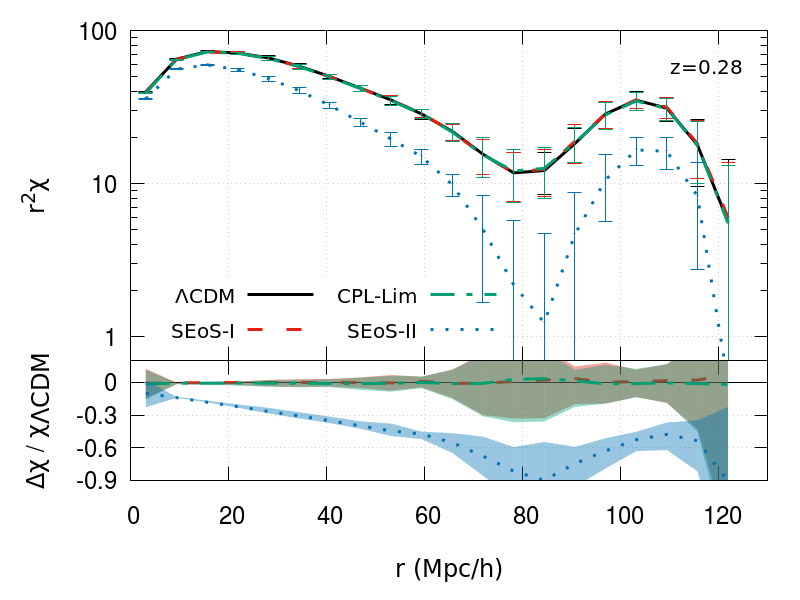
\includegraphics[width=0.33\textwidth,angle=0]{./plots/HS-50_Prom_2PCF_halos_Lb1024_out9} 
		% 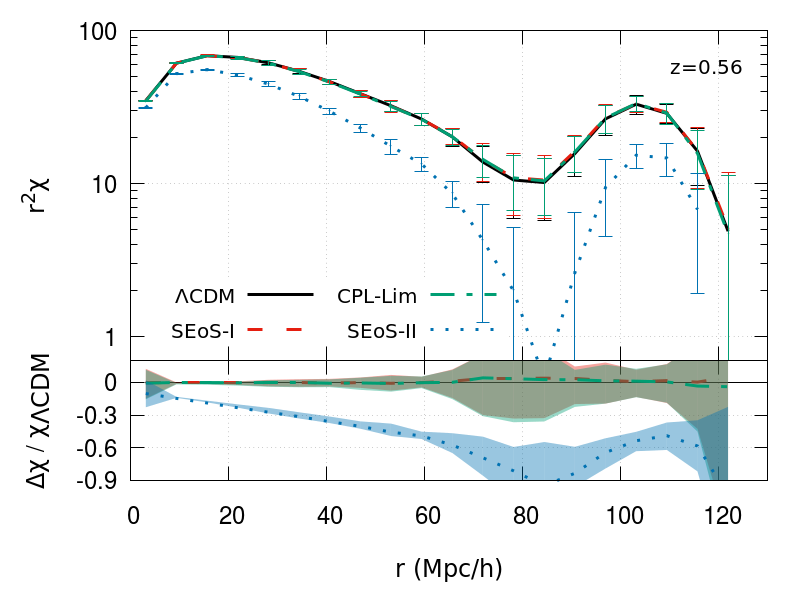
\includegraphics[width=0.5\textwidth,angle=0]{./plots/HS-50_Prom_2PCF_halos_Lb1024_out8}   
		%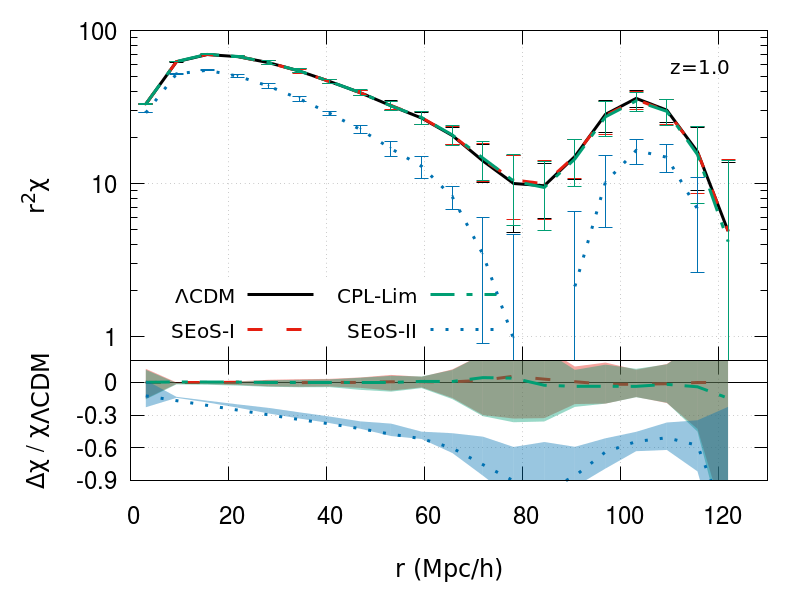
\includegraphics[width=0.33\textwidth,angle=0]{./plots/HS-50_Prom_2PCF_halos_Lb1024_out6} \\
		
	\end{tabular}
	
	\caption{2PCF for all the considered models at redshifts, $z = 0$, $0.28$, and $1.0$ after selecting halos with more than 50 particles. Their respective difference w.r.t. $\Lambda$CDM is shown in {\it middle} and {\it lower} panels. Shaded regions represent  1-$\sigma$ standard deviation, calculated from 5 realizations run with different random seeds. Note: A significant deviation is observed for SEoS-II model from the $\Lambda$CDM at all redshifts.}
	\label{fig:2PCF}
	% \end{center}
\end{figure*}


The two point correlation function (2PCF) remains one of the strongest tools to study the clustering of large scale structure either through galaxies or halos. For this work, we analyze the clustering of DM halos in real space for all the models. Our simulation settings of $L_{\rm box}$= $1024 h^{-1}{\rm Mpc}$ and $Np=1024^3$, allow us to trace up to the Baryon Acoustic Oscillation (BAO) scale.

The measurement of 2PCF between halos is performed with the code called Correlation Utilities and Two-point Estimates (CUTE) \cite{cutecode}\footnote{https://github.com/damonge/CUTE}. The correlation function we measure is estimated by the function:
\begin{equation}
\xi\left(r\right)=\frac{V_{\rm box}\times D_{h}D_{h}\left(r\right)}{V_{\rm bin}\left(r\right)\times N_{h}^{2}}-1,
\end{equation}
where $D_{h}D_{h}$ is the number of halo-halo pairs within a given separation bin of volume $V_{\rm bin}$, $N_{h}$ is the total number of halos in the box, and $V_{\rm box}$ is the volume of the simulation box, i.e., $V_{\rm box}=L_{\rm box}^3$. We set up 20 linearly spaced bins in the range of $r = 0-125~h^{-1} {\rm Mpc}$. For a statistically homogeneous and isotropic field, the halos are only correlated according to their relative distance, $r$. Thus, we present the result of 2PCF as function of $r$ in Figure (\ref{fig:2PCF}) for $z=0,\,0.28,\,1.0$.
%
%
Note that our results are based on the average over 5 realizations of the simulation we run for each model.
Similar to Figure (\ref{fig:pk_nonlinear}), the results are displayed in three panels (\ref{fig:2PCF}). The upper panel focuses on the full 2PCF, the middle one shows the relative difference of models w.r.t. $\Lambda$CDM, and the bottom panel shows a zoom of the relative difference to highlight the deviation of SEoS-I and CPL-lim from $\Lambda$CDM.

%, middle, and lower panels are focusing on the full 2PCF, relative difference of models w.r.t. $\Lambda$CDM, along with the error estimated from 5 realisations for each model, and the zoom in of middle plots to highlight the difference of SEoS-I and CPL-lim from $\Lambda$CDM respectively. 

From the upper panels of (\ref{fig:2PCF}), we observe the BAO feature at a scale of around $r\sim 100 h^{-1} {\rm Mpc}$ in all models, even with the limitation in resolution at those scales. The standard behaviors of the BAO feature are recovered, including the widening of the peak when it goes from high to low redshift.


A significant variation in the 2PCF is observed between SEoS-II and $\Lambda$CDM (see in the middle panels of (\ref{fig:2PCF})). As discussed before, the deviation between SEoS-II and $\Lambda$CDM is mainly governed by the difference in global cosmological parameters, i.e., $\Omega_{m0}=0.334$ and $H_{0} = 73.32$, instead of the $\Lambda$CDM values, $\Omega_{m0}=0.3089$ and $H_{0} = 67.74$. 
%
Thus, we draw the following conclusion. The low clustering signal revealed in the 2PCF of SEoS-II is due to the model with higher DM content leads to a faster growth of structures (see Figures \ref{fig:deltas} and \ref{fig:f_growth}), and ends up with denser but more widely spread halos. In addition, the DE-dominated epoch comes later in this model compared to $\Lambda$CDM, hence the structures tend to virialise earlier. This result also shows the sensibility of halo-clustering on the cosmological parameters. The difference in 2PCF of SEoS-II over $\Lambda$CDM reduces from $\sim 70\%$ at $r = 70 h^{-1} {\rm Mpc}$ to $\sim 20\%$ at $r = 20 h^{-1} {\rm Mpc}$. Note that the errors become relatively high after the scale, $r = 60 h^{-1} {\rm Mpc}$.



%Thus, we draw the following conclusion, the low clustering revealed in the 2PCF of SEoS-II is because the model with the higher DM content leading to a higher $H_{0$} overcoming the structure growth. In addition, DE dominated epoch comes later in this model compare to $\Lambda$CDM, hence the structures tend to virialise earlier. This result also shows us the sensibility of halo clustering on the cosmological parameters. The difference in 2PCF of SEoS-II over $\Lambda$CDM reduces from $\sim 70\%$ at $r = 70 h^{-1} {\rm Mpc}$ to $\sim 20\%$ at $r = 20 h^{-1} {\rm Mpc}$. Note that the errors become relatively high after the scale, $r = 60 h^{-1} {\rm Mpc}$.

 The bottom panel of (\ref{fig:2PCF}) shows that CPL-lim and SEoS-I models remain within  $\sim 1\%$ difference w.r.t. $\Lambda CDM$ up to the scales where the scatter is low, say $r = 60 h^{-1} {\rm Mpc}$. Hence, we conclude that it is challenging to trace the effect of dynamical DE using the halo clustering when we have a $\sim 2\%$ difference in the background expansion rate and the linear growth. We argue that including a larger number of simulations and increasing their accuracy with a larger number of particles and spatial resolution will improve further on this test. 
%---------- flag: UNDER CONSTRUCTION -------- reviewed by Mariana  until this point --------%
\subsection{Halo mass function}
\label{sec:massfunction}

%Another way to understand the growth of structures under different cosmological scenarios is through halos abundance, often referred as Halo mass function (HMF). HFM measures the number of halos per unit volume under certain range of mass bin, $M$ to $M+dM$ at some particular redshift.  We are using the halo mass definition of $M_{200} \equiv \frac{4\pi}{3}200\rho_{c}R^3_{200}$ which corresponds to halos enclosing $200$ times the critical density of our Universe and their corresponding radius $R_{200}$. Recall that halos are found using the \texttt{rockstar} halo-finder. 

%In principle, we know that the impact of dynamical DE is through the expansion history and the growth of structure. Depending on the behavior of EoS, $w(a)$ parameter, the expansion rate, $H(a)$ changes, thus the halos could be more or less clustered and accordingly the abundance changes in the structure formations. Subsequently, the structures can also take longer or lesser time period to form a bound structure under such situations. It is interesting to study their impacts on the halos abundance, often referred as Halo mass function (HMF). HFM measures the number of halos per unit volume under certain range of mass bin, $M$ to $M+dM$ at some particular redshift.  We use the halo mass definition of $M_{200} \equiv \frac{4\pi}{3}200\rho_{c}R^3_{200}$ which corresponds to halos enclosing $200$ times the critical density of our Universe and their corresponding radius $R_{200}$. Recall that halos are found using the \texttt{rockstar} halo-finder. 



\begin{figure*}
	\centering
	\begin{tabular}{cc}
		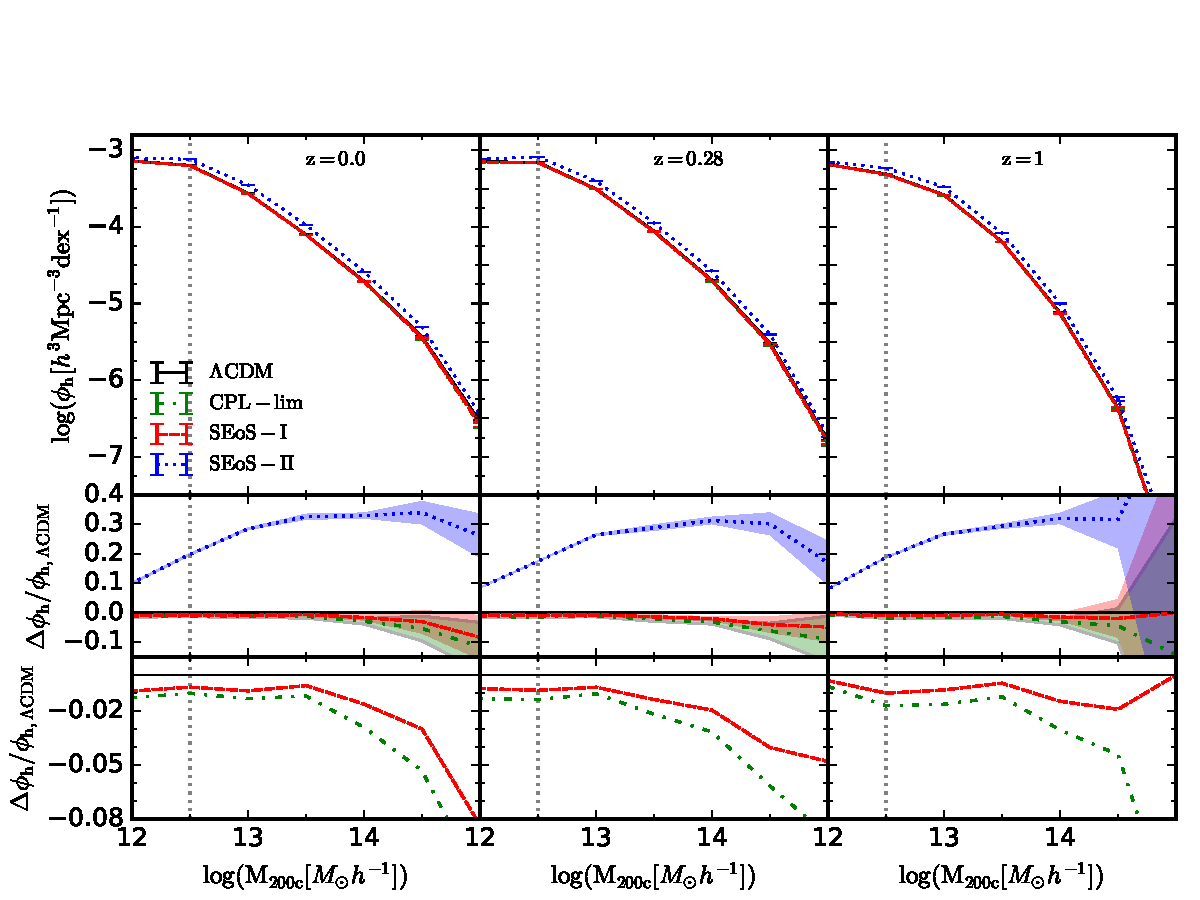
\includegraphics[width=1\textwidth,angle=0]{./plots/halo_mass_function_all_new.pdf} 
		% 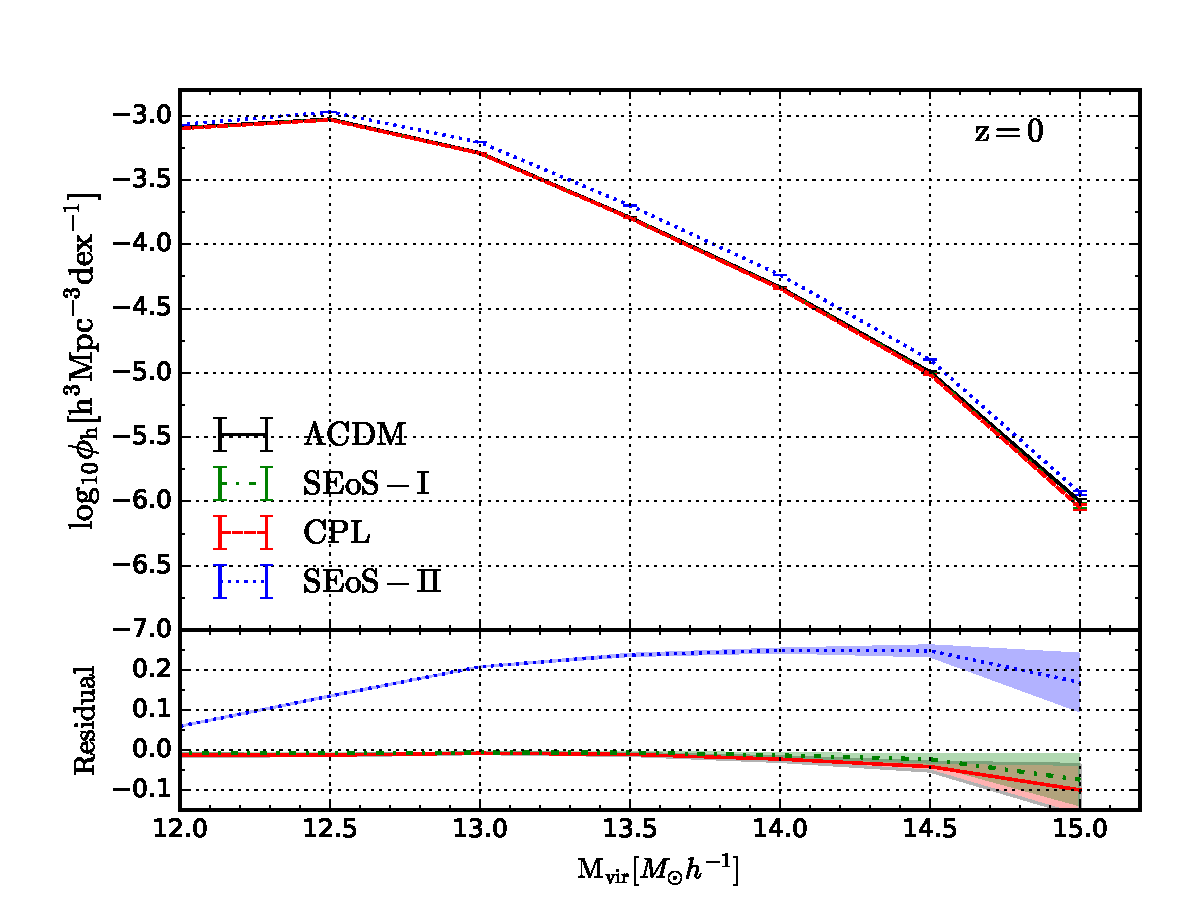
\includegraphics[width=0.33\textwidth,angle=0]{./plots/hmf_diff_11_z0.pdf}   
		% 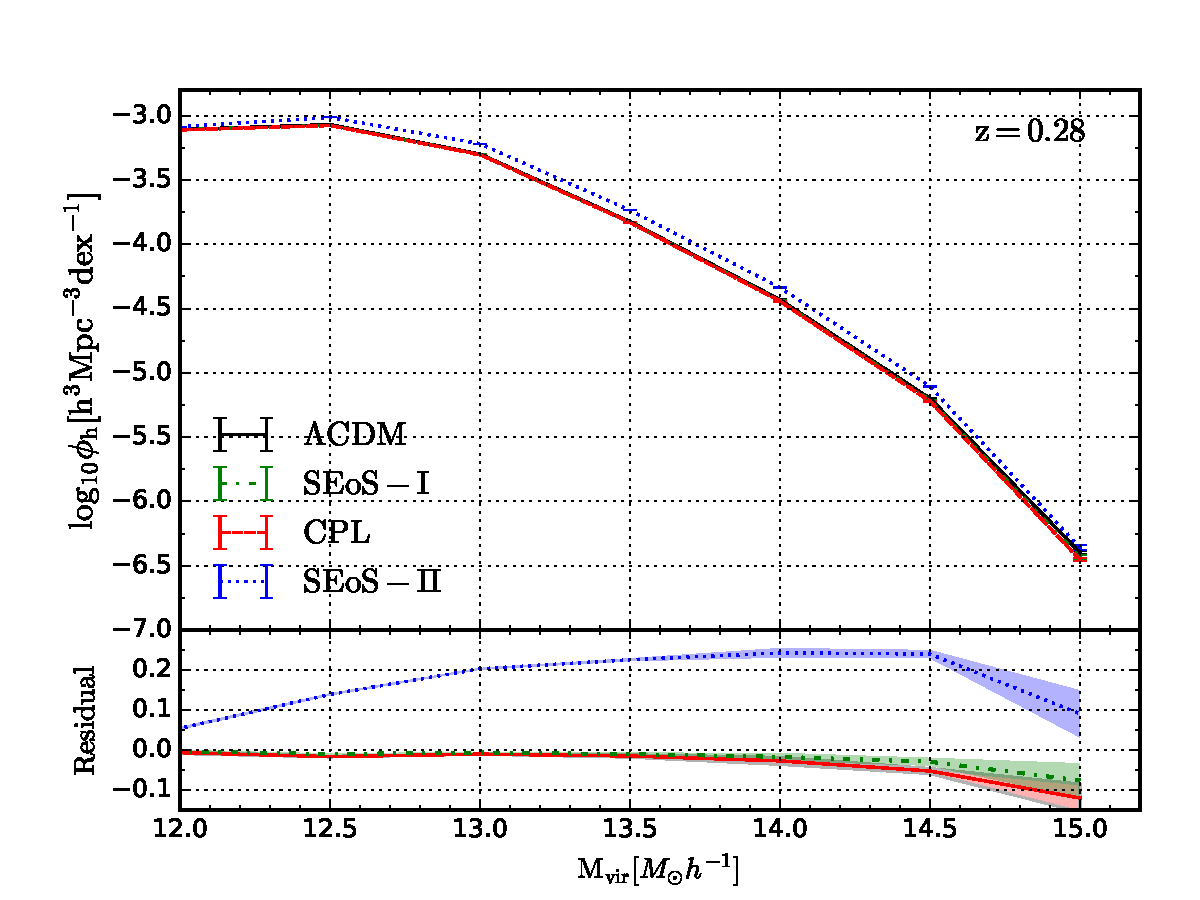
\includegraphics[width=0.33\textwidth,angle=0]{./plots/hmf_diff_9_z0p28.pdf} 
		
		% 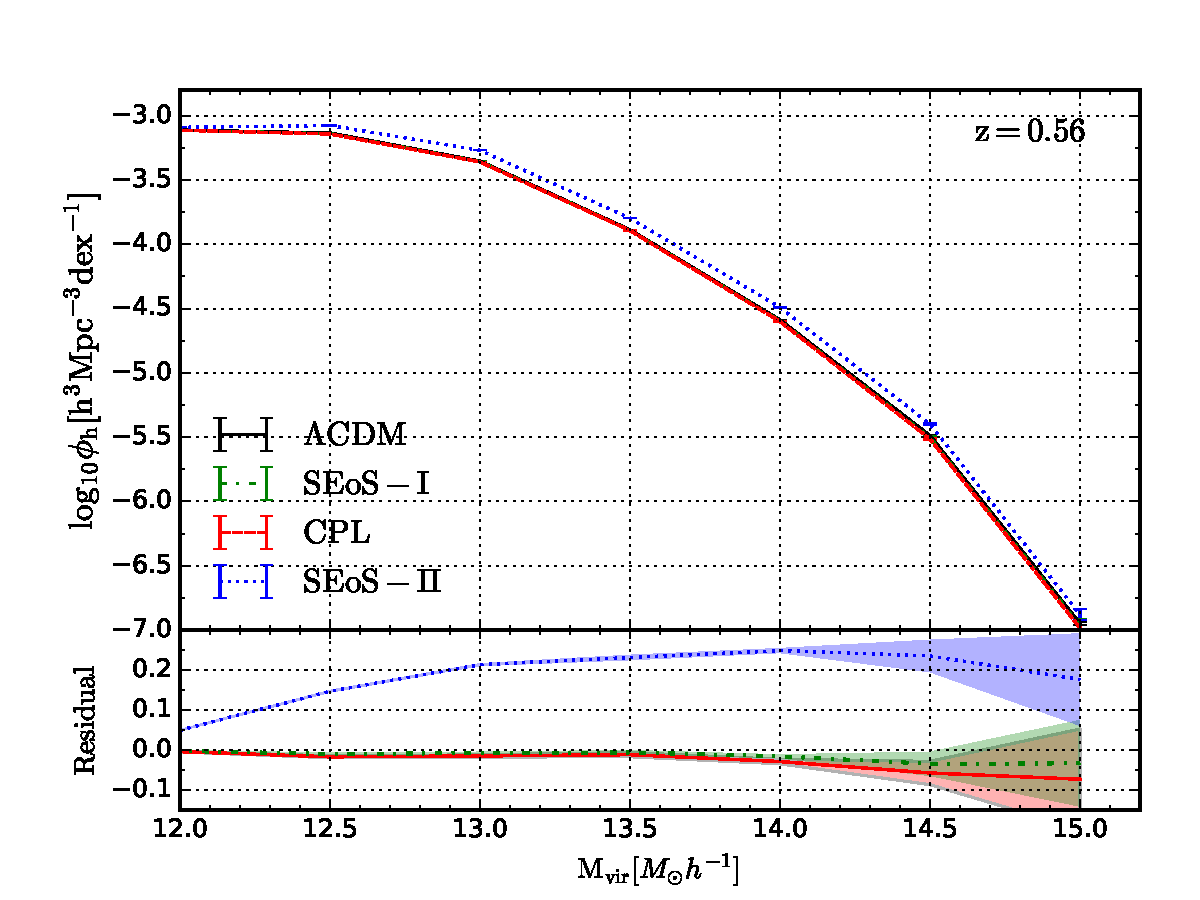
\includegraphics[width=0.5\textwidth,angle=0]{./plots/hmf_diff_8_z0p560.pdf}   
		% 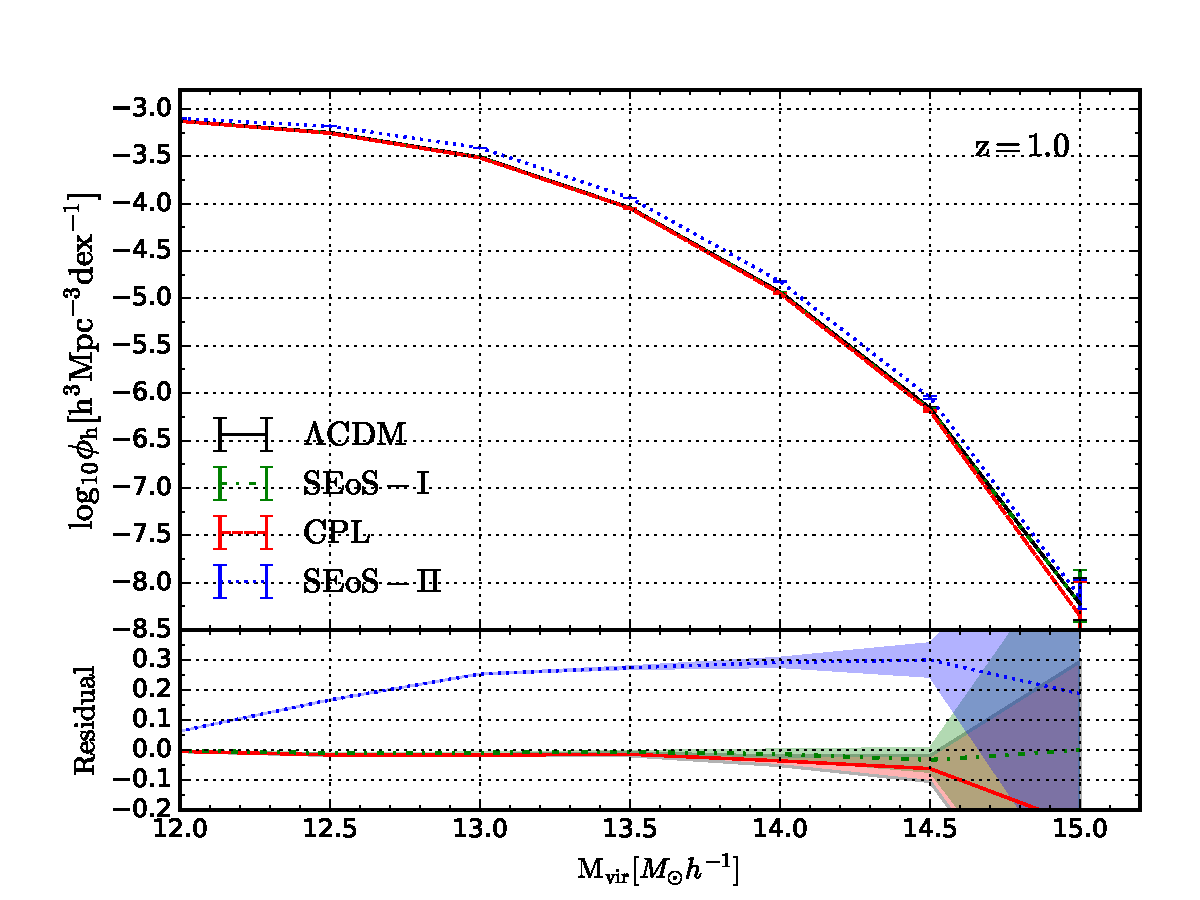
\includegraphics[width=0.33\textwidth,angle=0]{./plots/hmf_diff_6_z1p0.pdf} 
		
	\end{tabular}
	
	\caption{{\it Upper panels:} Differential halo mass functions for all the models at redshifts, $z = 0$, $0.28$, and $1.0$. {\it Middle panels}: The difference w.r.t. $\Lambda$CDM along with their one sigma standard deviation calculated from 5 realizations run under different random seeds (shaded regions). {\it Bottom panels}: Zoom-in plot of the second panel to highlight the differences between the CPL-lim and SEoS-I.
		%Note: A significant variation is observed for SEoS-II model from the $\Lambda$CDM at all redshifts.
	}
	\label{fig:HFM}
	% \end{center}
\end{figure*}


Depending on the behavior of DE, the structure we observed can be more or less clustered, subsequently, it will take less or longer time to form a gravitational bound structure. Such effect is studied via the Halo mass function (HMF). HFM measures the number of halos per unit volume under certain range of mass bin, $M$ to $M+dM$, at some particular redshift.  We use the halo mass definition of $M_{200} \equiv \frac{4\pi}{3}200\rho_{c}R^3_{200}$, which corresponds to halos enclosing $200$ times the critical density of our Universe, and their corresponding radius, $R_{200}$. 
%Note that halos are found using the \texttt{rockstar} halo-finder.

Figure (\ref{fig:HFM}) shows the mean differential HMF of 5 realizations for each model at redshifts $z = 0, 0.28$, and $1$. As expected, SEoS-I has the closest halo abundance to $\Lambda$CDM, followed by CPL-lim and SEoS-II. SEoS-II corresponds to an universe with $\Omega_{m0}=0.334$, so the number density of DM halos is expected to be larger than  for the other models. That is what we find in the HMF throughout the whole mass range and for all the redshift values considered (see the middle panels of Figure (\ref{fig:HFM})). A difference of $\sim 30\%$ in the HMF is observed between SEoS-II and $\Lambda$CDM in the mass range of $10^{13} M_{\odot}h^{-1} < M_{200}< 10^{15} M_{\odot}h^{-1}$. The difference is slightly reduced at both the low and high mass ends. This decrease in HMF at the high mass end is probably because of the difference in DE behavior. However, the most prominent effect is coming from the difference in the global cosmological parameters.% $\Omega_{m0}=0.334$ and $H_{0} = 73.32$.  

The bottom panel of Figure (\ref{fig:HFM}) highlights the main difference in HMF of SEoS-I and CPL-lim from $\Lambda$CDM. Noting that they share the same cosmological parameters: $\Omega_{m0}=0.3089$ and $H_{0} = 67.74$, the main difference is basically driven by the dynamics of DE. We observe that SEoS-I and CPL-lim have lower number of halos compared to $\Lambda$CDM at all mass scales and redshift values.
%  
The lower growth rate of matter overdensities in SEoS-I and CPL-lim w.r.t. $\Lambda$CDM results in a lower number of halos. One can infer from Figure \ref{fig:HFM} that the higher possibility of distinguishing between our  DE models and $\Lambda CDM$ lies in the high-mass halos. Particularly, looking at a mass scale of $M_{200}=10^{14.5} M_{\odot}h^{-1}$, a  significant difference of $\sim 3\%$ to $\sim 5\%$ is observed at $z = 0$ in SEoS-I and CPL-lim, respectively. However, going towards the high-mass limit comes at the cost of bigger uncertainty.
%
The difference in HMF reduces as we go from low to high redshift for both SEoS-I and CPL-lim. 
We argue that increasing the number of particles in the simulation  might help in reducing the uncertainty level and to increase the possibility of distinguish between the models. 
%Again, this is due to the fact that SEoS-I and CPL-lim have slightly higher expansion rates and thus, lower growth rate of matter densities then in $\Lambda$CDM, leading to end up with universe with less number of halos.

%The results of low HMFs observed in both SEoS-I and CPL-lim over $\Lambda$CDM at all mass scales is due to the fact that SEoS-I and CPL-lim have slightly higher expansion rates and thus, lower growth rate of matter densities over $\Lambda$CDM,


\section{Summary and Conclusions}
\label{sec:conclusions}

 In this paper, we presented a set of N-body simulations designed in the framework of dynamical DE models and analyzed their impact on the structure formation. In particular we studied the effect that a rapid dilution in the energy density of DE has on the growth of structure at cosmic scales. To this end, we assumed DE models with an equation of state, $w(z) = w_0 + w_i\frac{(z/z_T)^q}{1+(z/z_T)^q}$, where a  transition, controlled by the value of $q$, occurs between the fixed values $w_0\equiv w(z=0)$ and $w_i\equiv w(z\gg0)$, at an epoch given by $z_T$.

Specifically, we compared a DE model with a steep transition ($q=9.98$) at a late time ($z_T=0.28$)  versus the same model with a smooth transition ($q=1$) at a later time ($z_T=1$). The latter choice of parameters map our EoS to the Chevallier-Polarski-Linder parameterization \cite{Chevallier2001,Linder2003}. We referred to the the first case as the SEoS model, and  we further divided its study in two sets: SEoS-I and SEoS-II, depending on the cosmological parameters $\Omega_{m0}$ and $H_{0}$ used. The SEoS-I model is based on the Planck results (P15)\cite{Ade2016}: $\Omega_{m0}=0.3089$ and $ H_{0}=67.74$, as in $\Lambda$CDM and CPL-lim cases. The SEoS-II model considered $\Omega_{m0}= 0.334$, $H_{0} = 73.22$, the best fit values obtained in \cite{delaMacorra:2015aqf} along with the SEoS parameters. 
 

The structure formation under such DE scenarios was studied through the hacking of the approximated N-body simulation code called L-PICOLA \cite{Howlett:2015hfa}. %\cite{Tassev:2013pn,Tassev:2015mia}.  
The DE models were implemented via their expansion rates, and the DM perturbation solutions into the Lagrangian perturbations method employed in the code.   
%or initial conditions, we modified the 2LPTic code accordingly.
The simulations assume a box of length: $L_{\rm box}=1024 h^{-1}{\rm Mpc}$, and a number of dark matter particles of $N_{p} = 1024^3$ on a mesh, $N_{\rm mesh}= 1024$. In total, we ran 20 simulations, 5 realizations for each model to estimate the cosmic variance errors. Using the output of simulations, we analyzed the non-linear DM power spectrum, $P_{k}$, the number density of the gravitational bound halos, and halo clustering using the two-point correlation function. We discussed our results at redshifts, $z = 0, 0.28, 1$, since $z = 0.28$ and $z = 1$ are the transition redshifts for SEoS models and CPL-lim, respectively. 
%Halo catalogs are generated using the \texttt{rockstar} halo finder \cite{Behroozi2013} and the two point correlation functions were performed using the Correlation Utilities and Two-point Estimates code (CUTE) \cite{cutecode}. 
%The main results and conclusions from our studies are the following:

The main results and conclusions are as follows:
\begin{itemize}
\item %No significant imprint of the steep transition in DE field is found in the structure formation but we observed the impact of DE in the non-linear regimes. %
The calculated non-linear power spectra, $P_{k}$, of SEoS-I and CPL-lim models presented deficits in power w.r.t. $\Lambda$CDM throughout all $k$-modes. Such behaviour is expected due to the dynamics of DE, i.e., less negative values of the DE EoS and relatively larger expansion rate than in $\Lambda$CDM trigger a slowdown in the growth of structure. This result is consistent with the linear matter perturbations studies. The differences remain within $\sim 2\%$ and $\sim 3\%$ throughout all $k$ scales at $z = 0$ for SEoS-I and CPL-lim, with a slight increase at non-linear regimes. 
The reduction in the deviation from $\Lambda$CDM for higher redshift values is also showing the effect of the dynamics of DE. However, no significant imprint of the steep transition in the DE component is observed in the structure formation.
%As expected, SEOS-I is the closest one to $\Lambda$CDM, followed by CPL-lim and SEoS-II.

The $P_{k}$ of SEoS-II showed up relatively different behaviors. Specifically, a deficit in power at the linear scales and a closer  value to $\Lambda$CDM as it goes from linear to non-linear regimes. Such behavior in SEoS-II is expected for an universe containing more DM  $\Omega_{m0} = 0.334$ and with $H_{0} = 72.23$, instead of the standard values $\Omega_{m0} = 0.3089$, and $H_{0} = 67.74$. Thus, we conclude that the behavior of DE in SEoS-II model is sub-dominant compared to the effect of  changing $\Omega_{m0}$ and $H_{0}$.

\item We discussed how the differential halo mass functions (HMF) were effected by the behavior of DE models. The results of lower HMF observed in SEoS-I and CPL-lim as compared to $\Lambda$CDM at all mass-scales, occurred  as expected. The lower growth rate of matter densities in SEoS-I and CPL-lim w.r.t. $\Lambda$CDM results in a smaller number of bounded halos. The deviation w.r.t.$\Lambda$CDM of SEoS-I and CPL-lim reduces with the increase of redshift. The chances of distinguish between these models from $\Lambda$CDM increases at the high mass end. %Again, we observed reduced in deviation of SEoS-I and CPL-lim with the increase of redshifts.
The SEoS-II model has a value of $\Omega_{m0} = 0.334$, which in turns has a higher HMF, as predicted. The difference reaches up to $\sim 30\%$ deviation from $\Lambda$CDM at $ 10^{14.5}M_{\odot}h^{-1}$, at the considered redshifts.
%As such no variation is observed with redshift in case of SEoS-II.}
%are evolved with slightly higher expansion rates and thus,#
%Again, we observed reduced in deviation of SEoS-I and CPL-lim with the increase of redshifts.

\item We quantified the 2PCFs of SEoS-I and CPL-lim models and both remained within $\sim 1-2\%$ difference w.r.t. $\Lambda$CDM up-to $r = 60 {\rm Mpc} h^{-1}$. At larger scales, the accuracy of numerical experiments makes it challenging to state robust conclusions, but they behave in a consistent way. On the other hand, SEoS-II which was the best-fit model in  \cite{Jaber:2017bpx}, shows a significant difference throughout all $r$ scales. Such deviation reduces as we go from large to small scales in $r$. The deviation reaches up to $\sim 60\%$ at $r = 60 h^{-1} {\rm Mpc}$. We conclude that including the non-linear growth is critical in order to asses the viability of DE models.


\item Although not surprisingly for approximated simulations \cite{2016JCAP05051S}, the results of halo 2PCF and HMF might be biased by the ability of experiments to resolve halo mass and size, while $P_{k}$, in turn, uses the particle distribution. However the general trend of results is consistent across all tests.

\item We point out that having a tool to study LSS based on N-body simulations that run at low computational cost, and which simultaneously recovers the LSS accurately under the dynamical DE scenarios through L-PICOLA\cite{Howlett:2015hfa}, would  be deeply useful to understand the nature of DE. Particularly, it would prove very useful to provide constraints on DE models after running multiple sets of simulations on a wider range of cosmological and DE EoS parameters.

%Overall low clustering effects were depicted for SEoS-II at the redshift we considered but there is a significant deviation from $\Lambda$CDM through out all $r$ scales. Following the trend of higher clustering at low $r$ mode, then even lowering the clustering effect with the increase of $r$.}

\end{itemize}

On conclusion we state that our results from the non-linear structure formation are consistent with the behaviour of DE, their background and linear perturbation theories. Differences found in SEoS-I and CPL-lim models are directly driven by the DE dynamics. The deviation observed in SEoS-II is entangled with the effect of cosmological parameters and DE behavior. 

We recall that SEoS-II is the best-fitted model of SEoS found in \cite{Jaber:2017bpx}. %In  \cite{Jaber:2017bpx}  using the latest local Hubble constant measurement (\cite{Riess:2016jrr}) and the compressed CMB likelihood from Planck collaboration (\cite{Ade2016, mukherjee, planck15DE}) to constraint these models.
%make use of 
\cite{Jaber:2017bpx} used the observational points from the six-degree-field galaxy survey (6dFGS \cite{Beutler:2011hx}), Sloan Digital Sky Survey Data Release 7 (SDSS DR7 \cite{Ross:2014qpa}) and the reconstructed value (SDSS(R)  \cite{Padmanabhan2pc}), as well as the complete BOSS sample SDSS DR12 (\cite{Alam:2016hwk}), and the Lymann-$\alpha$ Forest (Ly$\alpha$-F) measurements from the Baryon Oscillation Spectroscopic Data Release 11 (BOSS DR11 \cite{Font-Ribera:2013wce}, \cite{Delubac:2014aqe}), along with the local Hubble constant measurement by (\cite{Riess:2016jrr}) and the compressed CMB likelihood from Planck collaboration (\cite{Ade2016, mukherjee, planck15DE}) to constraint the model. That being said, the large deviations w.r.t. $\Lambda$CDM in the non-linear structure formation found for SEoS-II, points out to the necessity  of extending the study of DE models beyond the linear regime.
%This implied that significant different observed in SEoS best fits values, could be improved further in future.
%The best fit values of model parameters and ($\Omega_{m0}=0.334$, $ H_{0}=72.23$) we used for SEoS-II obtained \cite{Jaber:2017bpx

%On conclusion, we state that having a tool to study LSS based on the N-body simulation that run at low computational costs and also simultaneously recovers the LSS accurately under the dynamical DE scenarios would be widely useful to understand the nature of DE. Particularly, this can provide the constrain on models parameters after running multiple sets of simulations based on the wide ranges of EoS and also on varying the cosmological parameters. The direct comparison with the clustering measurements from the up-coming surveys is one of our goals to perform after assigning galaxies to them. 


Note that our work was mainly focused on some particular DE parametrization, but the code can be easily extended to other dynamical DE models as long as the DE field remains homogeneous. Even though there is still room to further test SEoS models by increasing the number and accuracy of simulations, we are in progress of including other dynamical DE models such as the tachyon DE field and interacting DM-DE models in up-coming projects.  An strategy like the one presented in this paper is particularly appealing under the light of upcoming high accuracy galaxy surveys like DESI \cite{Aghamousa:2016zmz}.

\appendix
\section{The linear power spectrum}
\label{app:Pk_initial}
The initial linear power spectra, $P_{k,lin}$, at redshift $z_{in}=49$ from \texttt{CAMB}, used in the simulations are shown in Figure (\ref{fig:pk_initial}). The black solid and blue dotted lines correspond to the power spectra obtained with P15 ($\Omega_{m0} = 0.308$ and $H_{0} =0.6774$) and SEoS-II case: ($\Omega_{m0} = 0.334$ and $H_{0} =73.22$) respectively, see for other parameters in the table 1.  To compare, we aslo include the  power spectrum at $z = 0$, $P_{k,lin}$  computed from \texttt{CAMB} in black dash-dotted and red dashed lines for $\Lambda$CDM and SEoS-II cases respectively. We found that even at the initial power spectrum at $z_{in}=49$ there is an enhance in power at the high $k$ modes compare to inter-mediate scales, followed by the deficit in power in the low $k$ modes. The similar behavior is observed at $z = 0$ with slightly increase in different at high $k$ scales. These differences are expected and mainly due to the different in dark matter contained at the present time. 
%Such behaviors are well studied in literature with the $\Lambda$CDM model on varying the $\Omega_{m0}$, $w_{0}$ and $H_{0}$ values. We do observe a similar behavior in the non-linear power spectrum calculated on the output of our simulations, i.e., on comparing the SEoS-II to that of $\Lambda$CDM.

%\begin{figure}
%\centering 
%\hfill
%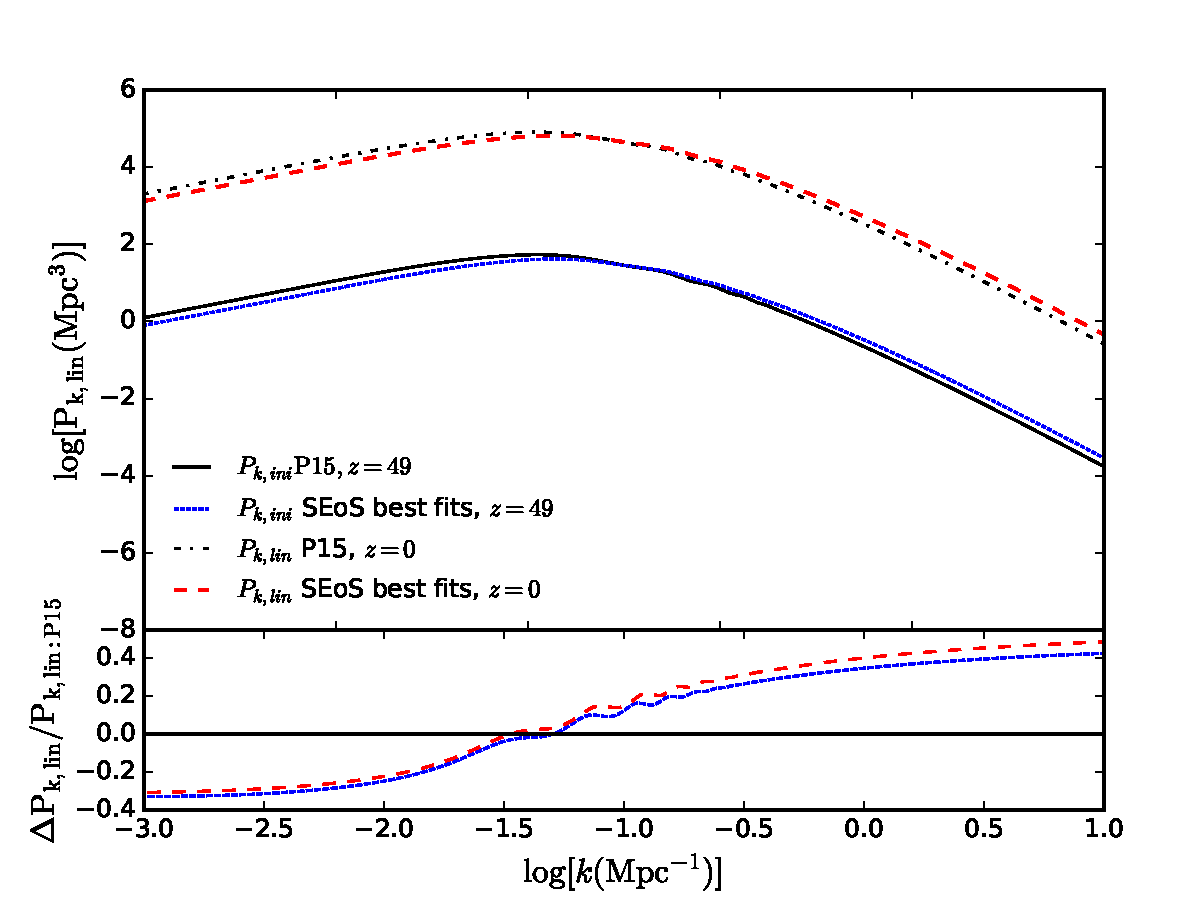
\includegraphics[width=0.6\textwidth,angle=0]{./plots/pk_camb_new.pdf}
%\caption{The initial linear power spectrum from \texttt{CAMB} at redshift $z_{in}=49$, used for our simulations. The black solid and blue dotted lines correspond to the power spectra with P15 cosmological values $\Omega_{m0} = 0.308$ and SEoS-II best fit values, $\Omega_{m0} = 0.334$ respectively. Their corresponding CAMB output at $z=0$ are also included for comparison in red dashed and black dash-dotted lines respectively. 
%\label{fig:pk_initial}}
%\end{figure}

\begin{figure}
\centering 
%\hfill
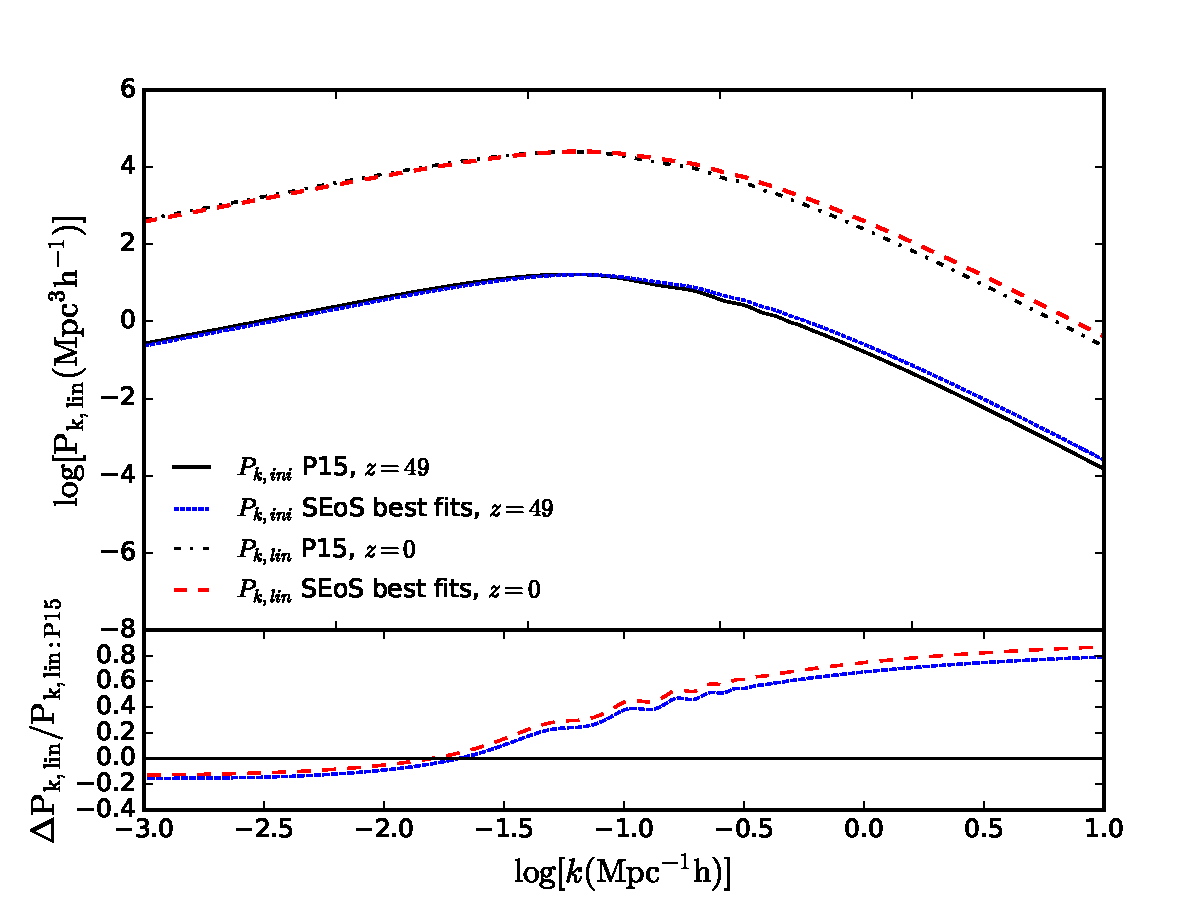
\includegraphics[width=0.6\textwidth,angle=0]{./plots/pk_camb_new2.pdf}
\caption{The initial linear power spectrum from \texttt{CAMB} at redshift $z_{in}=49$, used for our simulations. The black solid and blue dotted lines correspond to the power spectra with P15 cosmological values $\Omega_{m0} = 0.308$ and SEoS-II best fit values, $\Omega_{m0} = 0.334$ respectively. Their corresponding \texttt{CAMB} output at $z=0$ are also included for comparison in red dashed and black dash-dotted lines respectively. 
\label{fig:pk_initial}}
\end{figure}

\section*{Acknowledgements}
NCDevi thanks Hans Winther and Marc Manera for the fruitful discussions and feedback. 
NCDevi acknowledges support from a DGAPA-UNAM post-doctoral fellowship and CONACyT Fronteras de la Ciencia grant 281. %NCDevi thanks the support provide by LACEGAL during which this project is completed. 
NCDevi acknowledges support from the European Commission's Framework Programme 7, through the Marie Curie International Research Staff Exchange Scheme LACEGAL (PIRSES-GA-2010-269264) when main research of the work are obtained.
%
M. Jaber acknowledges the support of CONACYT graduate fellowship and that of the Polish Ministry of Science and Higher Education MNiSW grant DIR/WK/2018/12.  %LSST
%
Part of this work was supported by the ``A next-generation worldwide quantum sensor network with optical atomic clocks'' project, which is carried out within the TEAM IV programme of the Foundation for
 Polish Science co-financed by the European Union under the European Regional Development Fund.
 %TEAM
OV and G Aguilar acknowledge support from UNAM PAPIIT grant IN112518. G. Aguilar thanks support from a CONACyT graduate fellowship.
%We acknowledge support from Project IN103518 PAPIIT-UNAM and PASPA-DGAPA, UNAM.
M. Jaber and Axel de la Macorra acknowledge support from Project IN103518 PAPIIT-UNAM and A. De la Macorra of PASPA-DGAPA, UNAM. HV acknowledges support from IN101918 PAPIIT-UNAM Grant. The authors acknowledge DGTIC-UNAM for facilities on the Supercomputer MIZTLI at DGTIC-UNAM and also the ATOCATL Cluster Supercomputer of IA-UNAM.
The authors also thank Julio César Clemente for his help in setting up software in those supercomputer.  



\bibliographystyle{jhep}
\bibliography{refs}
\end{document}


\begin{figure*}
     \centering
     \begin{tabular}{cc}
        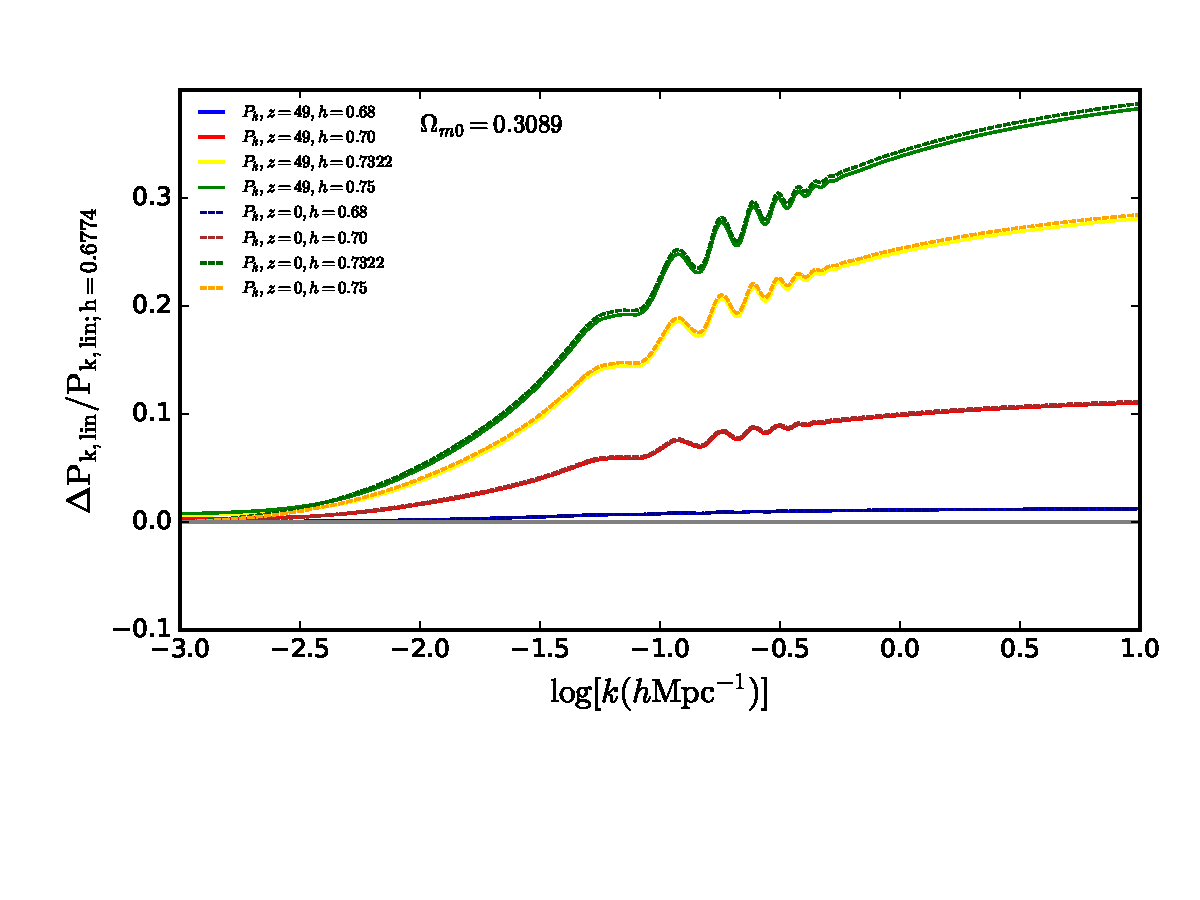
\includegraphics[width=\textwidth,angle=0]{./plots/pk_initial_varying_withh.pdf}   
%        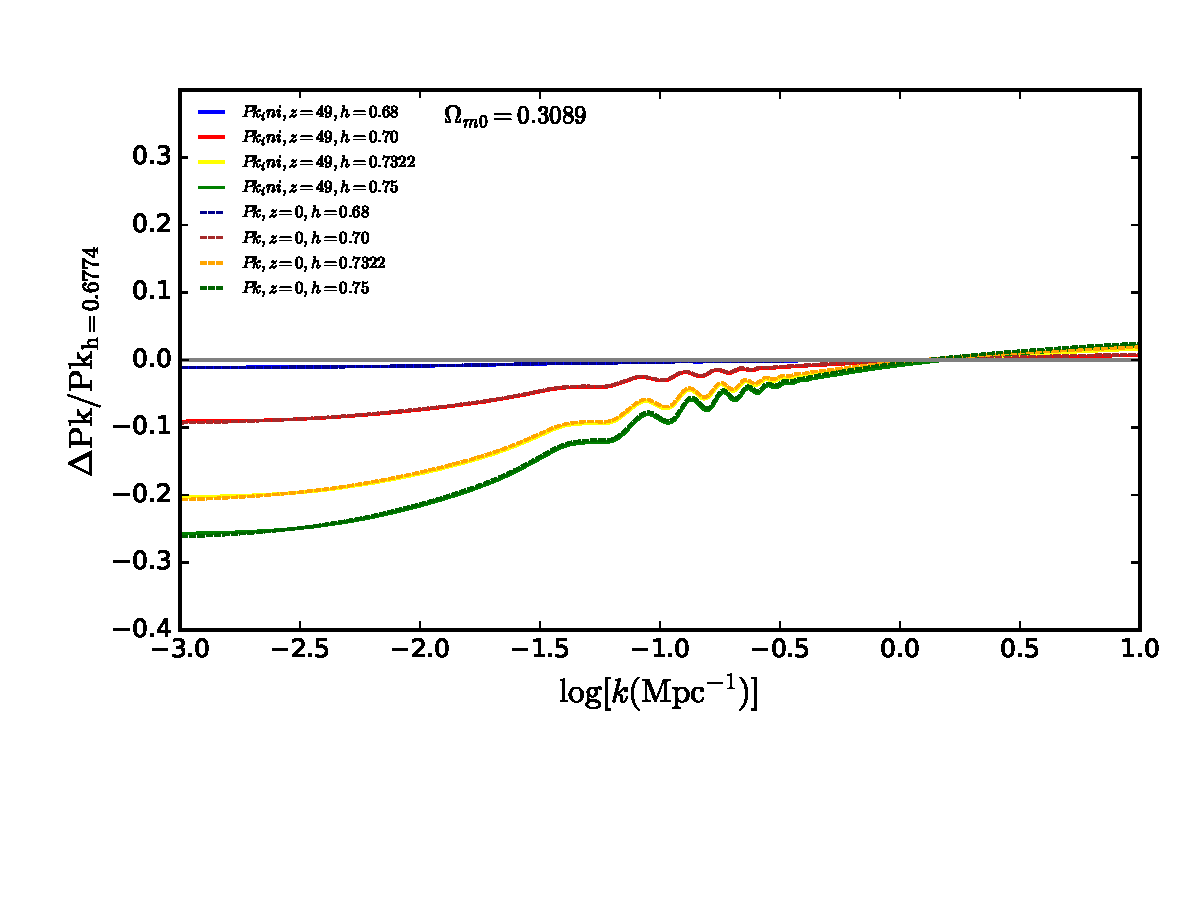
\includegraphics[width=0.5\textwidth,angle=0]{./plots/pk_initial_varying_h.pdf} \\

     \end{tabular}

\caption{{\it Left panel:} 
The linear power spectra for different values of $h$ for $\Lambda$CDM model from \texttt{CAMB} setting $\Omega_{m0}=0.3089$. The relative differences are calculated w.r.t. $h=0.6774$. {\it Right panel:} With the correction of each $h$ value.
}
\label{fig:pk_liner_h}
% \end{center}
\end{figure*}

\begin{figure}
\centering 
%\hfill
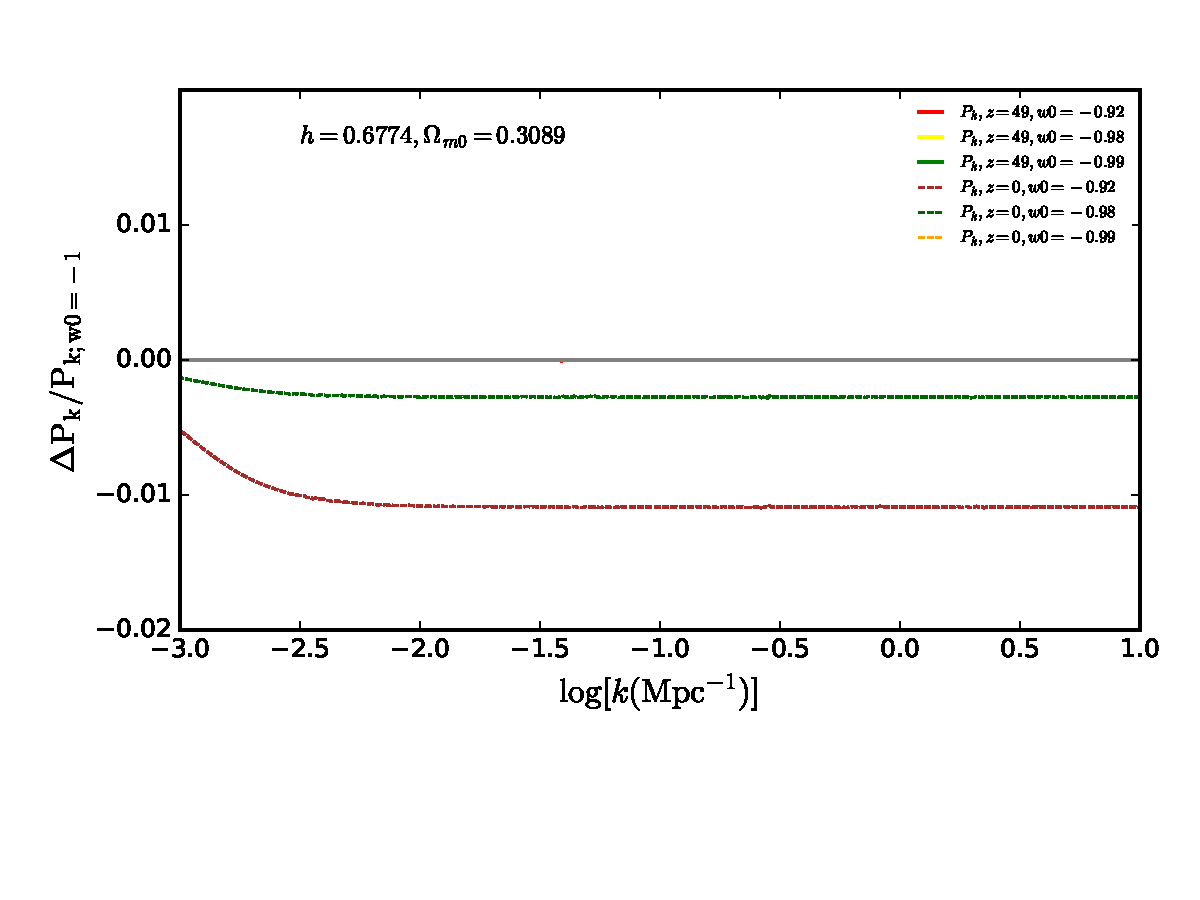
\includegraphics[width=\textwidth,angle=0]{./plots/pk_initial_varying_w0.pdf}
\caption{The linear power spectrum for a CPL like model, where $w0$ acts like $\Lambda$CDM equation of state $w$ at $z_{in}=49$ and $z=0$ from \texttt{CAMB}. With $w0=-0.99$(orange dotted),$-0.98$(green dotted),$-0.92$(red dotted) at $z=0$. The ratio is calculated with the power spectrum of $w0 =-1$. All of them are showing the same power spectrum at $z=49$. However, the up most different we took in the equation of state ($w0=-0.92$) and ($w0 = -1$) with different of $3\%$ shows a difference of $1\%$ on in the $P_{k,lin}$ 
\label{fig:pk_linear_w}}
\end{figure}



\begin{figure}
\centering 
%\hfill
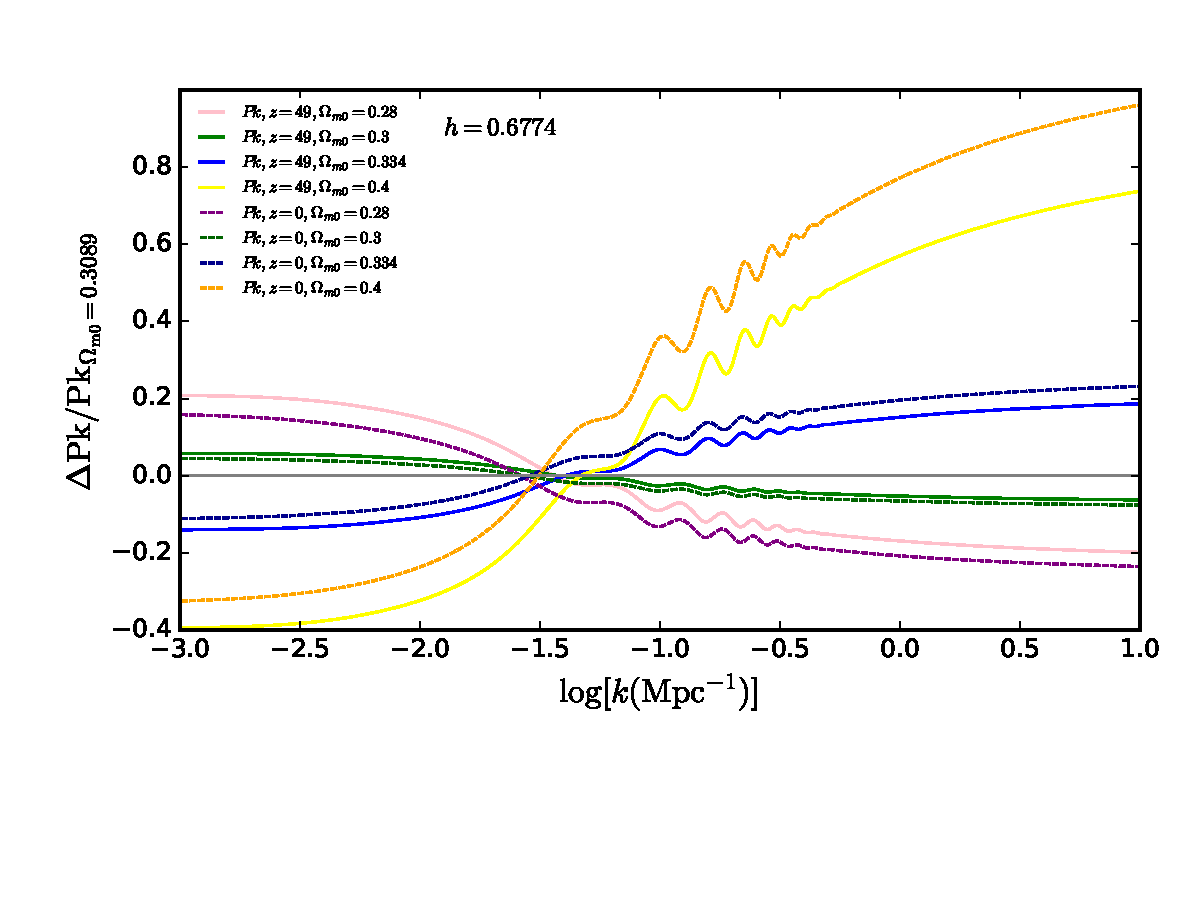
\includegraphics[width=0.6\textwidth,angle=0]{./plots/pk_initial_z0n49_varying_om_new.pdf}
\caption{The linear power spectra, $P_{k,lim}$ for the $\Lambda$CDM model at $z=0$ and $z = 49 $ from \texttt{CAMB}, on varying $\Omega_{m0}$ values. The blue lines correspond to the power spectra obtained for $\Omega_{m0} = 0.334$. The ratio is calculated w.r.t. $P_{k,lim}$ of $\Omega_{m0} =0.3089$.
\label{fig:pk_linear_om}}
\end{figure}


The $P_{k}$ of SEoS-II shows relatively different behavior with a deficit in power at the linear scales and the difference reduces when it goes from linear to non-linear regimes. A maximum deviation of $\sim 30\%$ at low scales (say at $k = 0.01{\rm Mpc}h^{-1}$) is observed in $P_{k}$ of SEoS-II. Such behavior is expected due to the different in the dark matter contained and $H_{0}$ for SEoS-II over $\Lambda$CDM. As such no significant impact of steep transition in DE field is found on the structure formation.
